\documentclass[letterpaper,12pt]{article}
\usepackage{amsmath}
\usepackage{graphicx}
\usepackage{epstopdf}
\usepackage{url}
\usepackage{multirow}
\usepackage{authblk}
\usepackage{color}  
\usepackage{enumitem}
\def\red{\color{red}}
\def\blue{\color{blue}}
\def\green{\color{green}}
\def\violet{\color{\frac{\lambda^a}{2}iolet}}
\def\orange{\color{orange}}


 % The package hyperref provides LaTeX the ability to create hyperlinks within the document. Comment out the next line to load document onto the arXiv.
\usepackage{hyperref}
\usepackage{xcolor}
% The package lineno adds line numbers to LaTeX documents.
\usepackage{lineno}

\usepackage[margin=0.65in]{geometry}

% Uncomment the following two lines to have line numbers printed in the document
\usepackage{lineno}
%\linenumbers

% Make author affiliations list small and italic
\renewcommand\Authfont{\footnotesize}
\renewcommand\Affilfont{\itshape\small}

\newcommand{\gx}{\textsc{GlueX}}


\date{June 12, 2020}

\title{\Large \textbf{Measuring the Neutral Pion Polarizability}\\
\large{Proposal Submitted to PAC 48} \\
\large{ Draft to GlueX Collaboration, Update 2}
}
% {\small  (A proposal to the 40$^\mathrm{th}$ Jefferson Lab Program Advisory Committee)}}


% This author list modified for the CPP proposal

%\title{Authors With Multiple Affiliations}
%\affiliation{First Institution/Department, Affiliation, City, Country }{FIRSTAFF}
%\affiliation{Second Institution/Department, Affiliation, City, Country }{SECONDAFF}
%\author{A.B. Firstauthor}{FIRSTAFF}
%\author{C. Coauthor}{SECONDAFF}
%\author[2]{D.E. Othercoauthor}{FIRSTAFF}

% \author{E.~Chudakov\thanks{Hall D Leader}}
% \author[1]{M.M.~Ito\footnote{Spokesperson}}
\author[1]{M.M.~Ito}
\author[1,2]{J.~Goity}
\author[1]{D.~Lawrence}
% \author[1]{D.~Lawrence$&^\ast$}
% \author[1]{E.S.~Smith$^\ast$\footnote{Contact Person, email: elton@jlab.org}}
\author[1]{E.S.~Smith\footnote{Contact Person, email: elton@jlab.org}}
\author[1]{B.~Zihlmann}

\author[3]{R.~Miskimen}
%\author[3]{R.~Miskimen$^\ast$}
\author[3]{I.~Larin}

\author[4]{A.~Aleksejevs}
\author[4]{S.~Barkanova}

\author[5]{A.~Austregesilo}

\author[6]{D.~Hornidge}

\author[7]{P.~Martel}

\affil[1]{Thomas Jefferson National Accelerator Facility, Newport News, VA}
\affil[2]{Hampton University, Hampton, VA}
\affil[3]{University of Massachusetts, Amherst, MA}
\affil[4]{Memorial University of Newfoundland, Corner Brook, Canada}
\affil[5]{Carnegie Mellon University, Pittsburgh, PA}
\affil[6]{Mount Allison University, Sackville, New Brunswick, Canada}
\affil[7]{Institute for Nuclear Physics, Johannes Gutenberg University, Mainz, Germany}








%\collaboration{The \textsc{GlueX}~Collaboration}


\begin{document}
\setlength{\parindent}{2em}

% Set narrow margins to allow full collaboration list to appear on single page
%\newgeometry{top=0.in,bottom=0.5in,right=0.5in,left=0.5in}

% Main title
\maketitle

% This prevents the page number from being printed on the title page. We do this
% because the bottom margin is so small the page number would otherwise be
% too far down.
\thispagestyle{empty}

\vspace{3cm}
{\large\textbf {Theoretical Support}} \\*[0.5cm]
\small{J.~Goity, \textit{Thomas Jefferson National Accelerator Facility, Newport News, Virginia and Hampton University, Hampton, Virginia}\\
A.~Aleksejevs,  \textit{Memorial University of Newfoundland, Corner Brook, Canada}\\
S.~Barkanova,  \textit{Memorial University of Newfoundland, Corner Brook, Canada}\\
S.~Gevorkyan,  \textit{Joint Institute for Nuclear Research, Dubna, Russia}\\
L.-Y.~Dai,  \textit{Hunan University, Changsha, Hunan, China}
}


% Set back to nominal margins (wider ones were set just for collaboration list)
\newgeometry{top=1.5in,bottom=1.5in,right=1.0in,left=1.0in}

%---------------------------------------------------------------------------------------------------------------
%--------------------------------- Abstract ------------------------------------------------------------------
%---------------------------------------------------------------------------------------------------------------
%\section{Abstract}
\begin{abstract}
This proposal presents our plan to make a precision measurement of the
cross section for $\gamma \gamma \rightarrow \pi^0 \pi^0$ via the
Primakoff effect using the GlueX detector in Hall D. The aim is to
significantly improve the data in the low $\pi^0\pi^0$ invariant mass
domain, which is essential for understanding the low-energy regime of
Compton scattering on the $\pi^0$. In particular, the aim is to obtain
a first-ever experimental determination of the neutral pion
polarizability $\alpha_\pi - \beta_\pi$, which is one of the important
predictions of chiral perturbation theory and a key test of chiral
dynamics.  Our goal is to measure
$\sigma(\gamma\gamma\rightarrow\pi^0\pi^0)$ to a precision of about
5.1\%, which will determine the combination of
$\alpha_{\pi^0}-\beta_{\pi^0}$ to a precision of 39\%. We expect this
experiment to run concurrently with the previously approved experiment
to measure the charged pion polarizability (CPP) \cite{CPPexp} in
Hall~D.
\end{abstract}


\newpage

\tableofcontents 

\newpage

\setlength{\parskip}{0.1in}

%---------------------------------------------------------------------------------------------------------------
%--------------------------------- Introduction ------------------------------------------------------------------
%---------------------------------------------------------------------------------------------------------------
\section{Introduction}

Electromagnetic polarizabilities are fundamental properties of
composite systems such as molecules, atoms, nuclei, and hadrons
\cite{Holstein:1990qy}. Whereas { form factors} provide information
about the ground state properties of a system, polarizabilities
provides information about the excited states of the system, { and are
  therefore determined by the system's dynamics}.
%For atomic systems polarizabilities are on the order of the atomic
%volume.  For hadrons the polarizabilities are much smaller than the
%volume, typically of the order of $10^{-4}$ fm$^3$, because of the
%greater stiffness of the QCD force as compared to the electromagnetic
%force.
Measurements of hadron polarizabilities provide an important test
point for Chiral Perturbation Theory, dispersion relation approaches,
and lattice calculations. Among the hadron polarizabilities, the
neutral pion polarizability ranks of paramount importance because it
tests fundamental symmetries, in particular chiral symmetry and its
realization in QCD.  Indeed, the non-trivial (non-perturbative) vacuum
properties of QCD result in the phenomenon of spontaneous chiral
symmetry breaking, giving rise to the Goldstone Boson nature of the
pions.  In particular, the Goldstone Boson nature of the $\pi^0$
manifests itself most notably in its decay into $\gamma\gamma$ and
also in its electromagnetic polarizabilities, which according to ChPT
can be predicted to leading order in the expansion in quark
masses.


Hadron polarizabilities are best measured in Compton scattering
experiments where, in the case of nucleon polarizabilities, one looks
for a deviation of the cross section from the prediction of Compton
scattering from a structureless Dirac particle.
In the case of pions, the long lifetime of the charged pion permits
experiments of low energy Compton scattering using a beam of high
energy pions scattering on atomic electrons. On the other hand, the
short lifetime of the neutral pion requires an indirect study of low
energy Compton scattering via measurements of the process $\gamma
\gamma \rightarrow \pi^0 \pi^0$, a method that can also be applied to
the charged pion (CPP) and for which a proposal in Hall D is already
approved \cite{CPPexp}.

This proposal presents a plan to make a precision measurement of the
$\gamma \gamma^* \rightarrow \pi^0 \pi^0$ cross section using the
GlueX detector in Hall D.  The measurement is based on the Primakoff
effect which allows one to access the low $W_{\pi^0\pi^0}$ invariant
mass regime with a small virtuality of the $\gamma^*$ representing the
Coulomb field of the target. The central aim of the measurement is to
drastically improve the determination of the cross section in that
domain, which is key for constraining the low energy Compton amplitude
of the $\pi^0$ and thus for extracting its polarizability.  At
present, the only accurate measurements exist for invariant masses of
the two $\pi^0$s above 0.7 GeV, way above the threshold 0.27 GeV. The
existing data at low energy were obtained in $e^+ e^- \to \pi^0\pi^0 $
scattering in the early 1990's with the Crystal Ball detector at the
DORIS-II storage ring at DESY \cite{Marsiske:1990hx}.

Meanwhile, theory has made significant progress over time, with
studies of higher chiral corrections 
\cite{Bellucci:1994eb,Gasser:2005ud,Aleksejevs:2014eea} and with the
implementation of dispersion theory analyses which serve to make use
of the higher energy data
\cite{Oller:2008kf,Dai:2014zta,Dai:2014lza,Moussallam:2013una}. It is
expected that the experimental data from this proposal, together with
those theoretical frameworks, will allow for the most accurate
extraction of the $\pi^0$ polarizabilities to date.


%---------------------------------------------------------------------------------------------------------------
%---------Theoretical predictions for the charged pion polarizability --------------------------
%---------------------------------------------------------------------------------------------------------------
\section{Theoretical predictions for the neutral pion polarizability}
The low energy properties of pions are largely determined by  their nature as
the Goldstone Bosons of spontaneously broken chiral symmetry in QCD,
and are described in a model independent way by the framework of
Chiral Perturbation Theory (ChPT) (Gasser and Leutwyler
\cite{Gasser:1983yg}), which implements a systematic expansion in low
energy/momentum and in quark masses.  In particular the pions' low
energy electromagnetic properties can serve as tests of their
Goldstone Boson (GB) nature. One such a case is the $\pi^0\to
\gamma\gamma$ decay, which at the same time tests its GB nature and
the chiral anomaly. Another case is low energy Compton scattering on
pions: at low energy the Compton differential cross section can be
expanded in powers of the photon energy and expressed in terms of the
corresponding pion charge form factor (for charged pion) and the electric
and magnetic
polarizabilities, where the latter give the order $\omega^2$ terms in
the Compton cross section, being $\omega$ the photon energy. The
polarizabilities appear as deviations
of the pions from point like particles, and thus result from carrying
out the chiral expansion to the next-to-leading order. For both
charged an neutral pions the polarizabilities are fully predicted at
leading order in quark masses, and thus represent a sensitive test of
chiral dynamics. For the charged pions, at $O(p^4)$ ChPT predicts that
the electric and magnetic polarizabilities ($\alpha_{\pi^+}$ and
$\beta_{\pi^+}$) are related to the charged pion weak form factors
$F_V$ and $F_A$ in the decay $\pi^+ \rightarrow e^+ \nu \gamma$
\begin{equation}\label{alpha_and_beta}
\alpha_{\pi^+} = -\beta_{\pi^+} \propto \frac{F_A}{F_V} = \frac{1}{6} ( l_6 - l_5 ),
\end{equation}

\noindent where $l_5$ and $l_6$ are low energy constants in the Gasser
and Leutwyler effective Lagrangian \cite{Gasser:1983yg}.  Using recent
results from the PIBETA collaboration for $F_A$ and $F_V$
\cite{Bychkov:2008ws}, the $O(p^4)$ ChPT prediction for the charged
pion electric and magnetic polarizabilities is given by:
\begin{equation}\label{one_loop}
\alpha_{\pi^+} = -\beta_{\pi^+} = (2.78 \pm 0.1) \times 10^{-4}~{\rm fm}^3.
\end{equation}

\begin{figure}[h]
\begin{center}
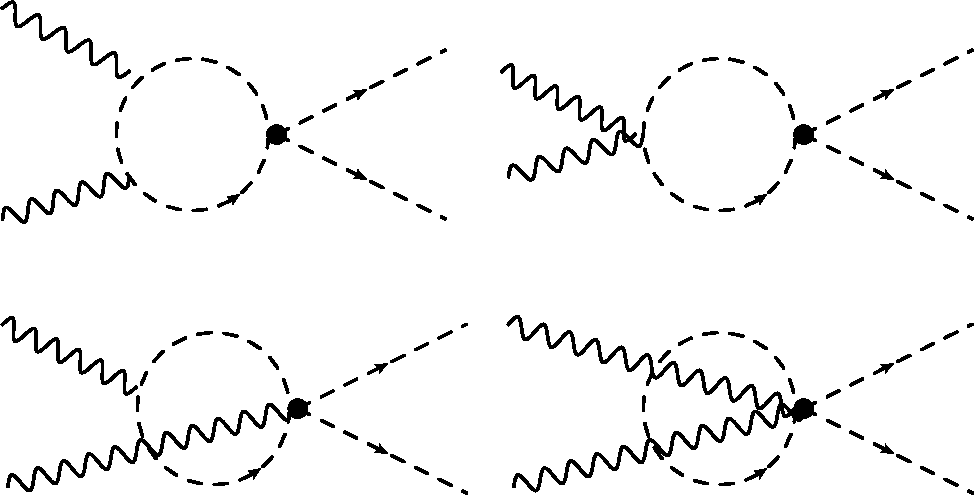
\includegraphics[height=6cm,angle=0]{figures/DiagramsChPT.pdf}
\end{center}
\caption{Diagrams contributing to Compton scattering off the $\pi^0$.
\label{fig:digrams}}
\end{figure}


In the case of the neutral pion, the polarizabilities are determined
by the one loop chiral contributions (see Fig.\,\ref{fig:digrams})
which are calculable, free of unknown parameters, and given only in
terms of the fine structure constant, the pion mass and the pion decay
constant:
\begin{eqnarray}
\alpha_{\pi^0}+\beta_{\pi^0}&=&0\nonumber\\
\alpha_{\pi^0}-\beta_{\pi^0}&=&-\frac{\alpha}{48 \pi^2 M_\pi F_\pi^2}\simeq -1.1\times 10^{-4}~{\rm fm}^3
\end{eqnarray}
However, there is a range of predictions beyond
NLO and the experimental test of these important predictions is very
challenging. In particular, the polarizabilities drive the very
low energy regime of Compton scattering on the $\pi^0$ as there is no
Thomson term, so one would expect that it would be easier to determine
them than in the charged pion case.  However, direct
Compton scattering on the $\pi^0$ is experimentally inaccessible due
to its short lifetime, and therefore it is necessary to resort to the
process $\gamma\gamma\to \pi^0\pi^0$ of this proposal. In addition, ChPT
indicates that the
polarizabilities are smaller in the case of the neutral pion, about a
third of their value for the charged pion, i.e. somewhere between
$-1.7\times 10^{-4}~{\rm fm}^3$ and $-1.9\times 10^{-4}~{\rm fm}^3$,
depending on the model used to estimate higher order effects in the chiral
expansion. The challenge is therefore to measure the
cross section for $\gamma\gamma \to \pi^0\pi^0$ with sufficient
accuracy at low invariant mass $W_{\pi\pi}$ so that one can infer the
low-energy Compton amplitude and extract the polarizabilities. The demand for
accuracy is required in order to allow for the extrapolation of the Compton
amplitude from the kinematics of $\gamma\gamma \to \pi^0\pi^0$ to   low energy
Compton scattering, something that is at present impossible with the poor
accuracy of the only available data from the Crystal Ball experiment \cite{Marsiske:1990hx}.
 


For
this purpose, the theoretical foundations have been laid in works
studying $\gamma\gamma\to \pi^0\pi^0$ both using ChPT (Bellucci et al
\cite{Bellucci:1994hx,Bellucci:1994eb}, Gasser et al
\cite{Gasser:2005ud}, Aleksejevs and Barkanova
\cite{Aleksejevs:2014eea}) and dispersion theory (Oller and Roca
\cite{Oller:2008kf}, Dai and Pennington
\cite{Dai:2014zta,Dai:2014lza}, Moussallam
\cite{Moussallam:2013una}). In particular, in ChPT at the next-to-next
to leading order, which provides the higher order quark mass
corrections to the polarizabilities, some of the low energy constants
need to be fixed and for that a significantly more accurate
measurement of the $\gamma\gamma\to \pi^0\pi^0$ cross section is
needed than available presently.

Accurate measurements of the cross section near threshold combined
with data for $W_{\pi\pi}>0.6$ GeV will provide the necessary input
for performing a full theoretical analysis, combining dispersion
theory with and without inputs from ChPT at low energy. This is a well
established method which has been used to analyze $\pi\pi$
scattering and also to the very problem of the $\gamma\gamma \to \pi^0\pi^0$
process, where numerous works have been steadily improved the theoretical
dispersive analysis, to mention a
few \cite{Donoghue:1993kw,Oller:2007sh,Oller:2008kf,Moussallam:2013una,Dai:2016ytz}.
Through such an analysis it will be possible to determine,
via combination with ChPT, the low energy Compton amplitude and
extract the   combination $\alpha_\pi-\beta_\pi$. The
latter extraction represents a challenge as shown in
Fig.\,\ref{fig:previousdata}, where the polarizabilities have a small
direct effect on $\gamma\gamma\to \pi\pi$.  Calculations by Dai and
Pennington (Table II) \cite{Dai:2016ytz} indicate that a 1.3\%
determination of $\sigma(\gamma\gamma\rightarrow\pi^0\pi^0)$ will
determine the combination of $\alpha_{\pi^0}-\beta_{\pi^0}$ to a
precision of 10\%. 
%The preliminary study done by Aleksejevs and Barkanova for this proposal in relativistic ChPT with SU(3) input indicate that sensitivity could be even better depending on specific kinematics; the full evaluation is in progress. 
In general, the
determination of the accuracy one can get for $\alpha_\pi-\beta_\pi$
based on a more accurate measurement as the one proposed here is still
an issue being currently studied theoretically, with J. L.  Goity and
A. Aleksejevs and S. Barkanova forming a group to take a lead on the project. 
At present a theoretical study based on the S-wave dominance below
$W_{\pi\pi}\sim 0.8 GeV$ and dispersion theory has allowed to represent the two
Compton amplitudes $A$ and $B$ in the physical domain of the experiment. The
study of the extrapolation to low energy Compton kinematics is under study, in
particular the issues related to the stability of the dispersive analysis. This
study is expected to provide a more accurate estimate on the sensitivity with
which the experiment will allow for the determination of the polarizability
$\alpha-\beta$.


%However, even 10\% precision would still be sufficient to difference between various models and facilitate extraction of low-energy constants, and thus a highly desirable result for theory.

\begin{figure}[ht]
\begin{center}
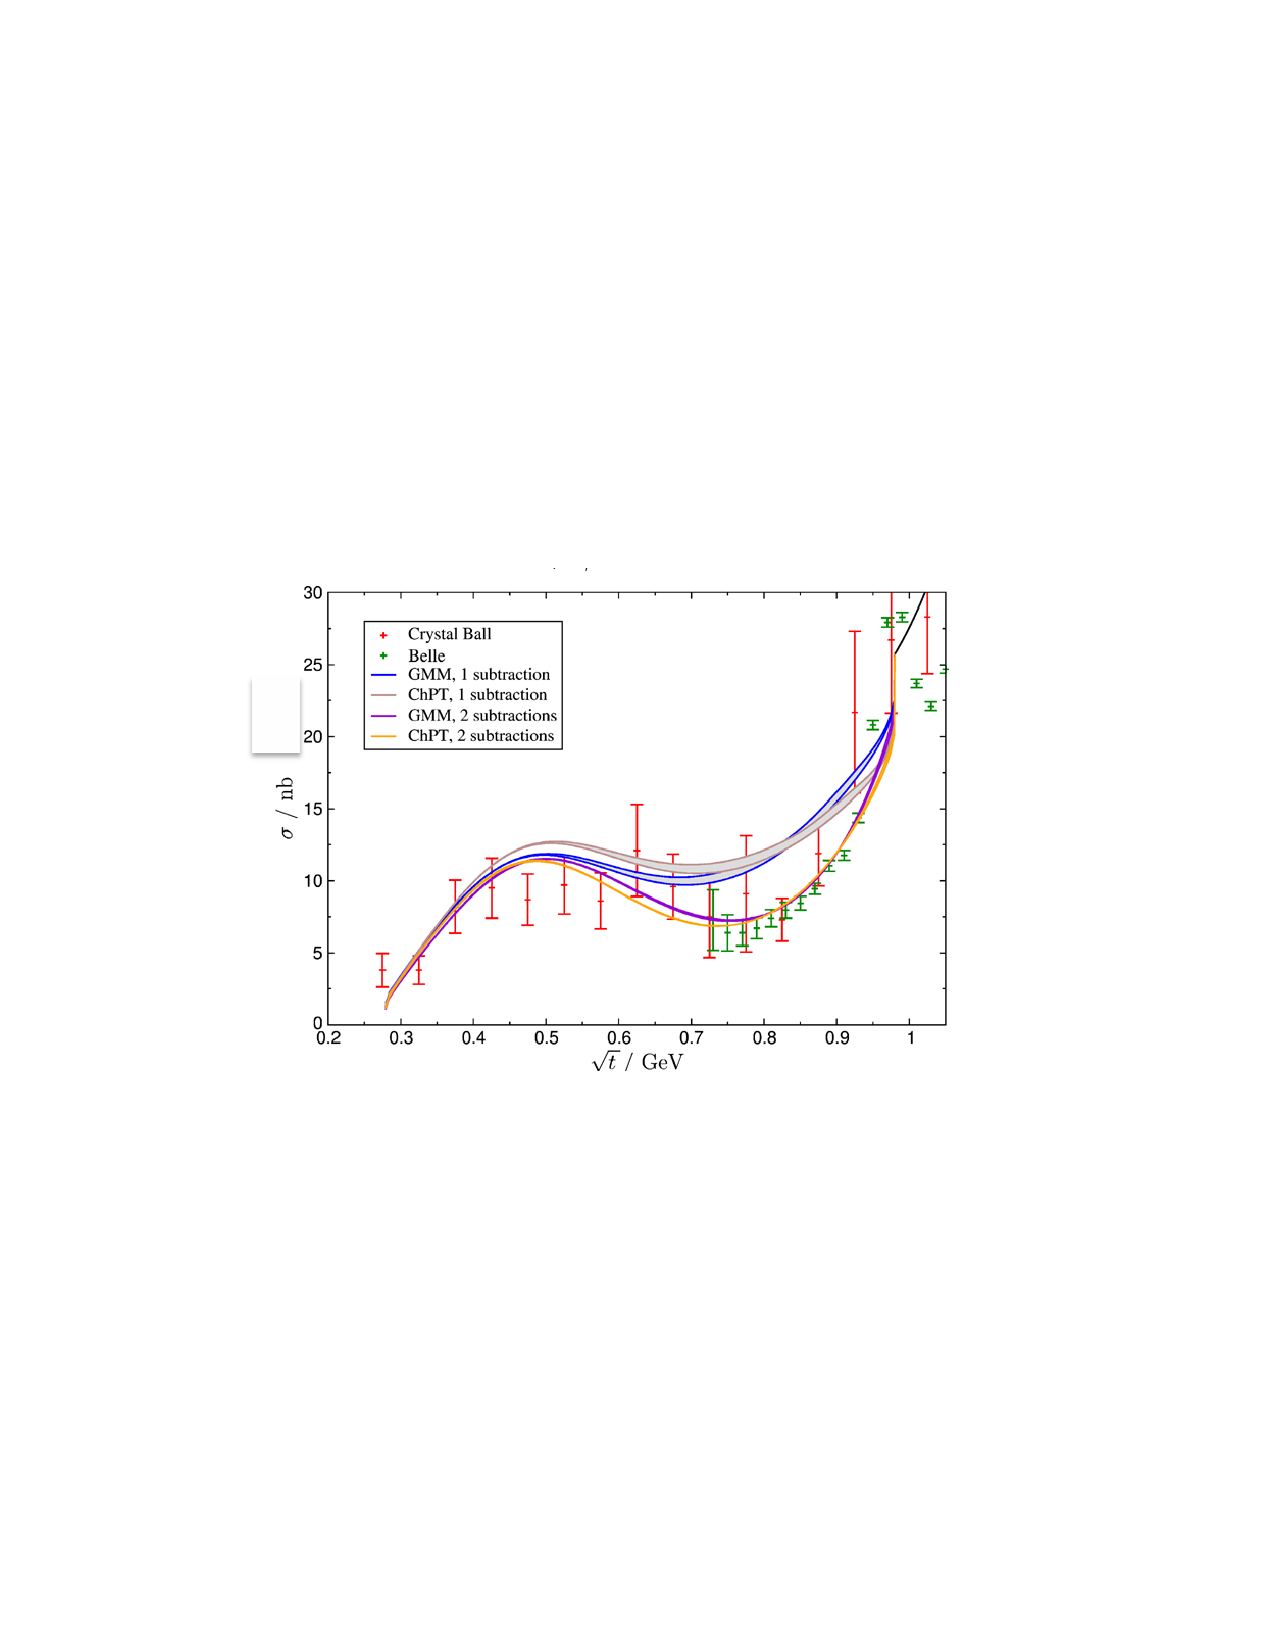
\includegraphics[height=5cm,angle=0]{figures/Fig-TP-2pr.pdf}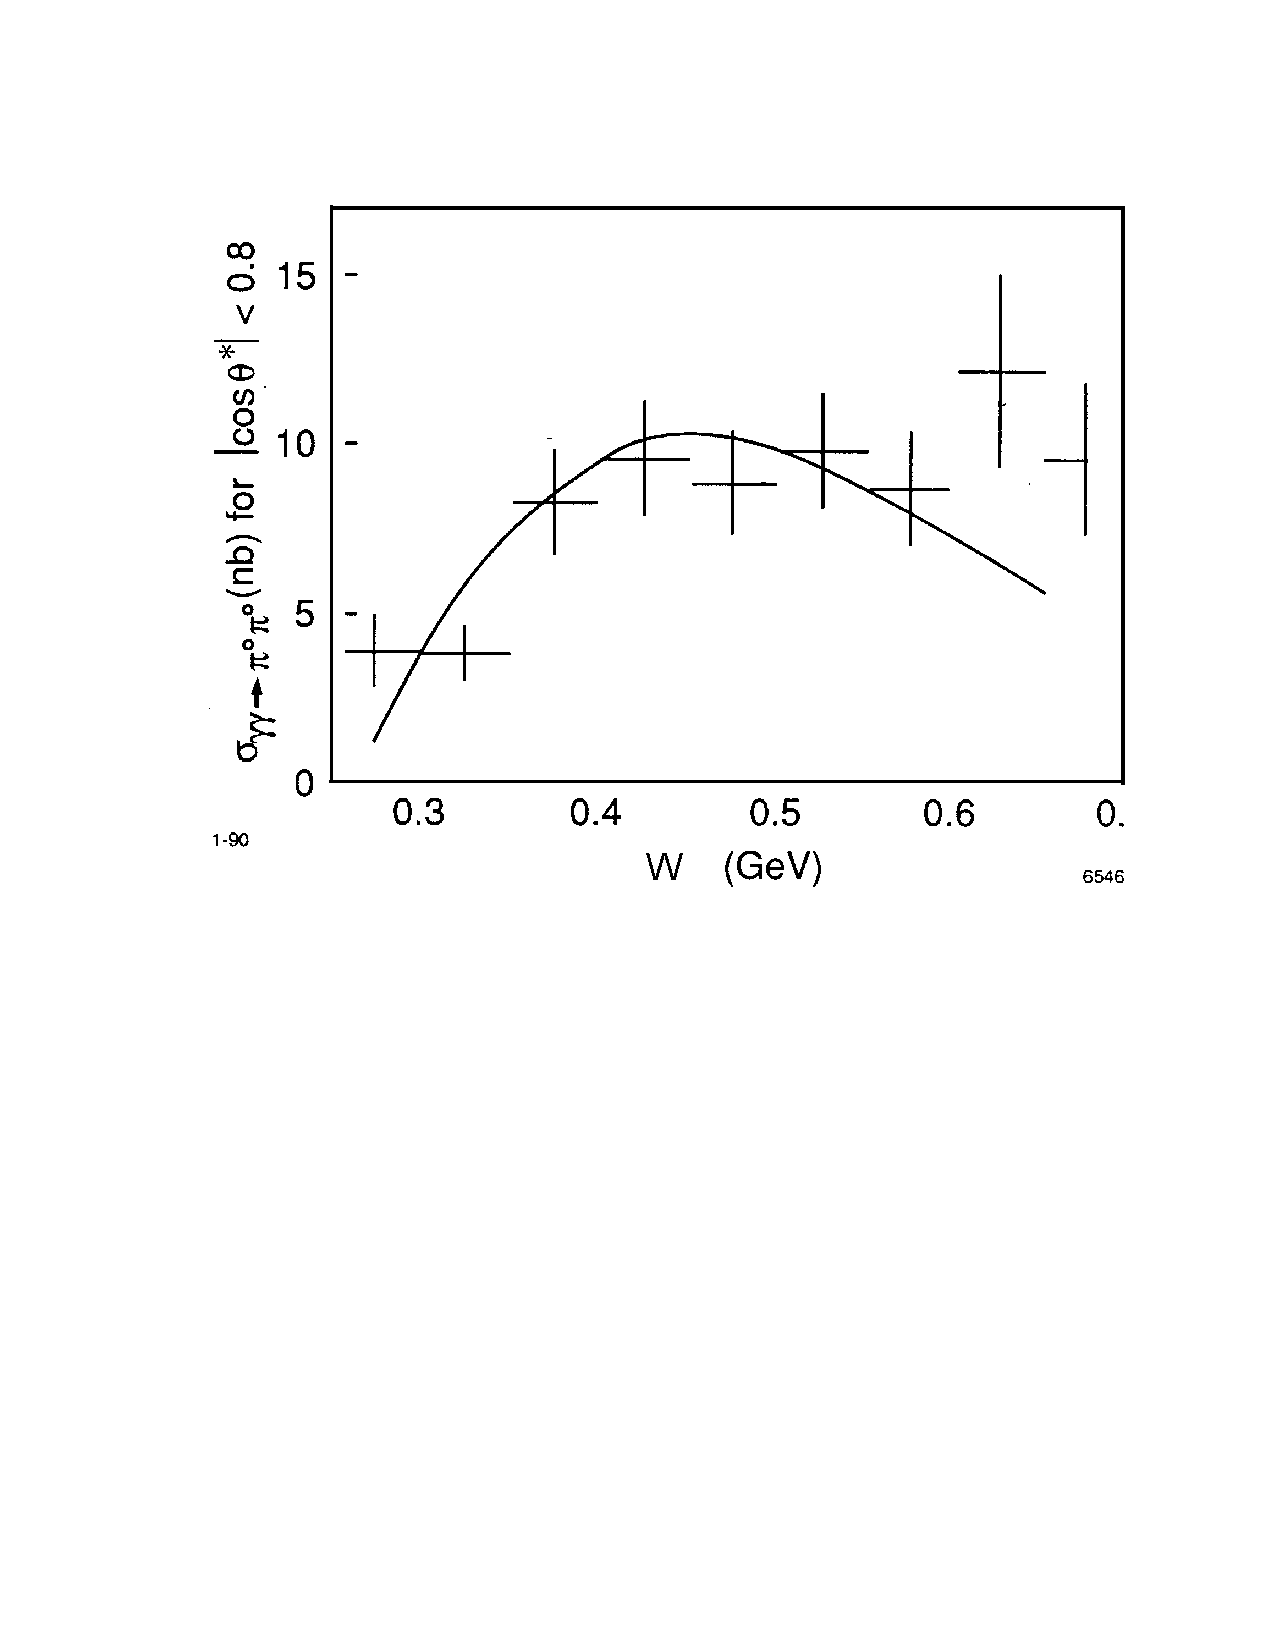
\includegraphics[height=5cm,angle=0]{figures/XBall.pdf}\\
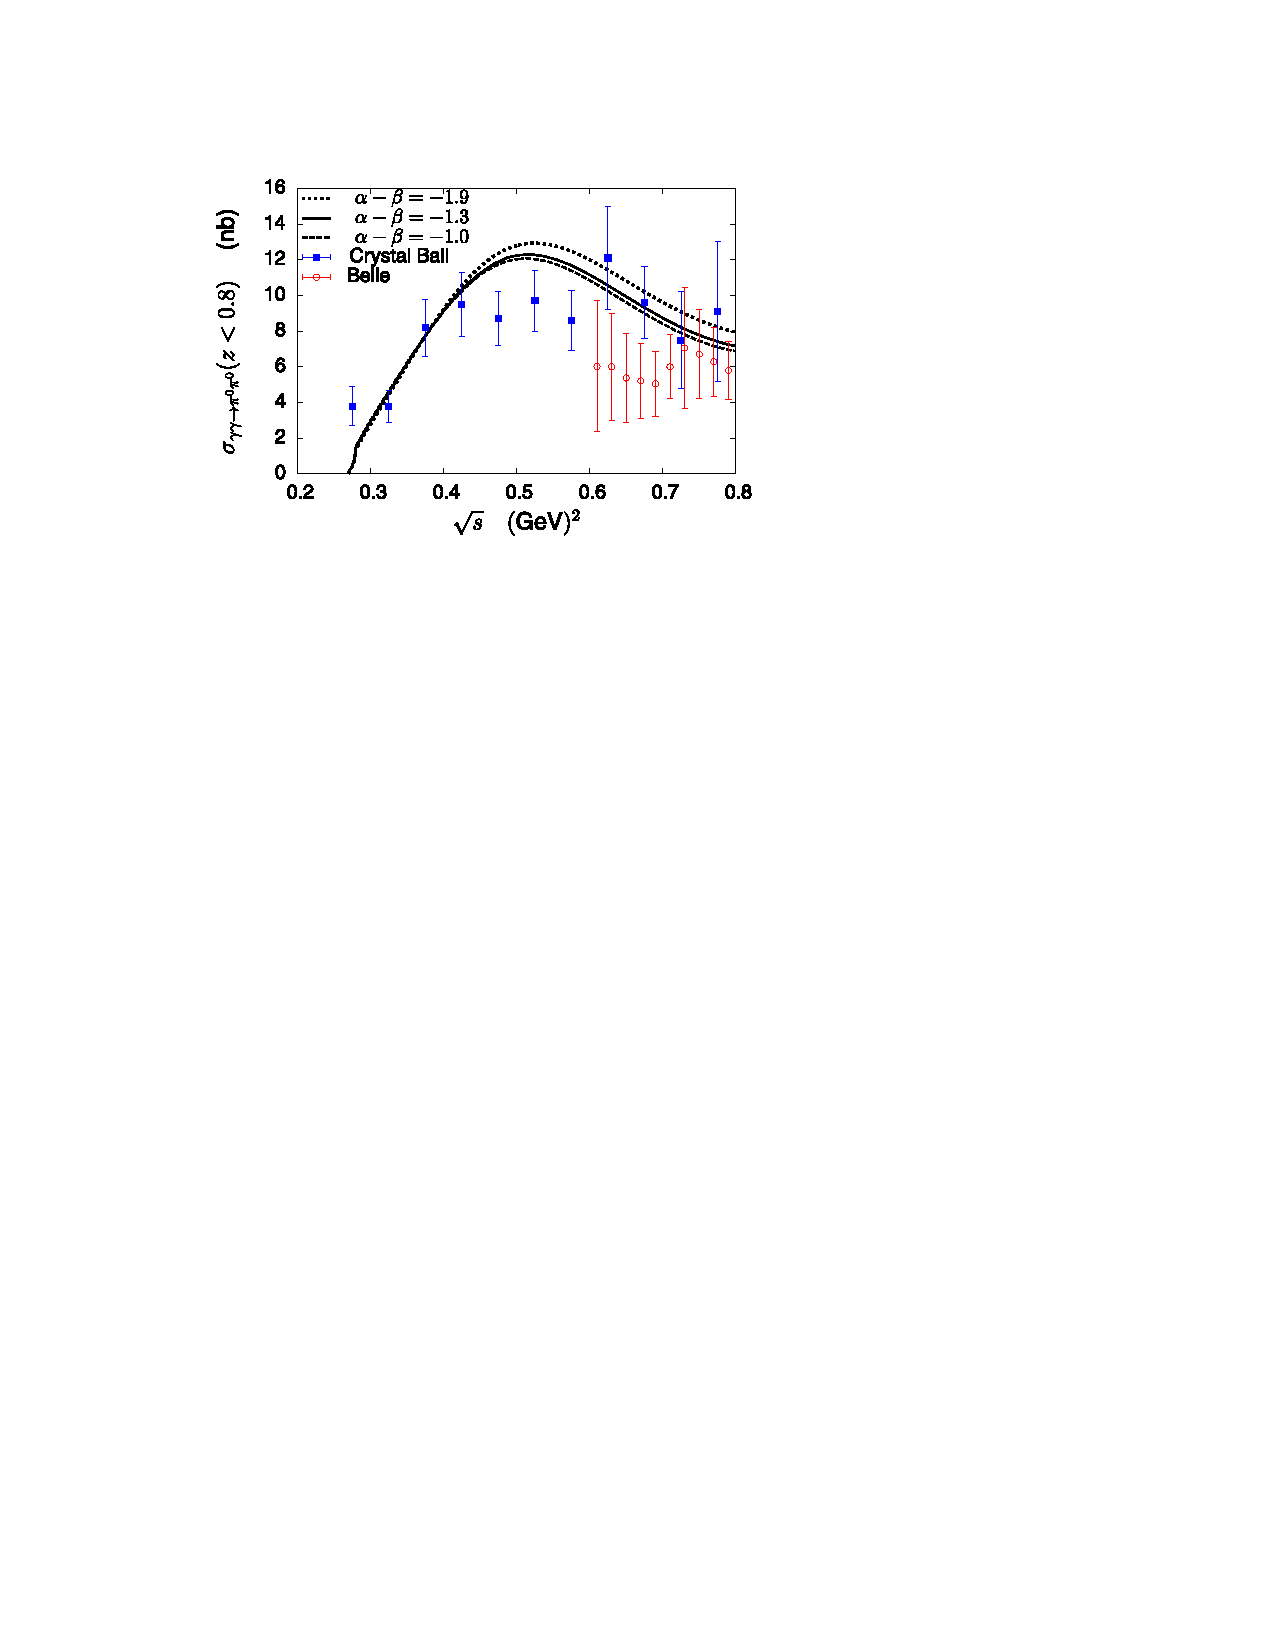
\includegraphics[height=6cm,angle=0]{figures/Fig-TP-5.pdf}\i
%\includegraphics[height=6cm,width=8cm,angle=0]{gA-Mpi-LHPC-band.pdf}
\end{center}
\caption{Left panel: experimental status; right panel: results from the 1990
XBall experiment. The lower panel shows the effect of $\pi^0$ polarizabilities
on the cross section ($\sqrt{s}=W_{\pi\pi}$) \cite{Moussallam:2013una} .
\label{fig:previousdata}}
\end{figure}

\section{Past Measurements}
Past measurements of the $\gamma\gamma\to \pi^0\pi^0$ cross section are shown Fig.\,\ref{fig:CrystalBall_BELLE_data} and  with theoretical curves in Fig.\,\ref{fig:previousdata}. The data can be
summarized as follows: 
\begin{enumerate}
    \item 
In the early 1990's measurements were made in $e^+e^-$ collisions at DESY
with the Crystal Ball detector at the DORIS-II storage ring \cite{Marsiske:1990hx}, which are the only
available data for $W_{\pi\pi}<0.6{\rm~ GeV}$. 
\item In 2008-2009, measurements were carried out by BELLE
for $0.6{\rm~ GeV}<W_{\pi\pi}<4.0 {\rm~ GeV}$ \cite{Mori:2007bu,Uehara:2008ep,Uehara:2009cka}. Two data sets were produced with different selection cuts on $|\cos{\theta^*}|$.
\end{enumerate}
As mentioned above, several works have made use of dispersion theory methods
(Oller and
Roca \cite{Oller:2008kf}, Dai and Pennington \cite{Dai:2016ytz}, and
in particular Moussallam \cite{Moussallam:2013una} who performed the
dispersive analysis where one of the photons has non vanishing
virtuality, which is particularly important for our case.) with those
available data. In particular these methods give results for the cross
section at small $W_{\pi\pi}$, but the poor accuracy of the data in
that region does not serve as a useful constraint that could improve
those analyses. On the other hand, the ChPT calculations carried out
at NNLO (Bellucci et al \cite{Bellucci:1994hx,Bellucci:1994eb} ) can
only be fitted to the low $W_{\pi\pi}$ data, and thus the uncertainty
in the determination of low energy constants is rather large. It is therefore
expected that accurate data at low $W_{\pi\pi}<0.6{\rm~ GeV}$ will
have a very big impact on both theoretical approaches, which together
may allow for an accurate description of the low energy Compton
amplitude, and for a first time experimental determination of the
polarizability.

\begin{figure}[tbh]
\begin{center}
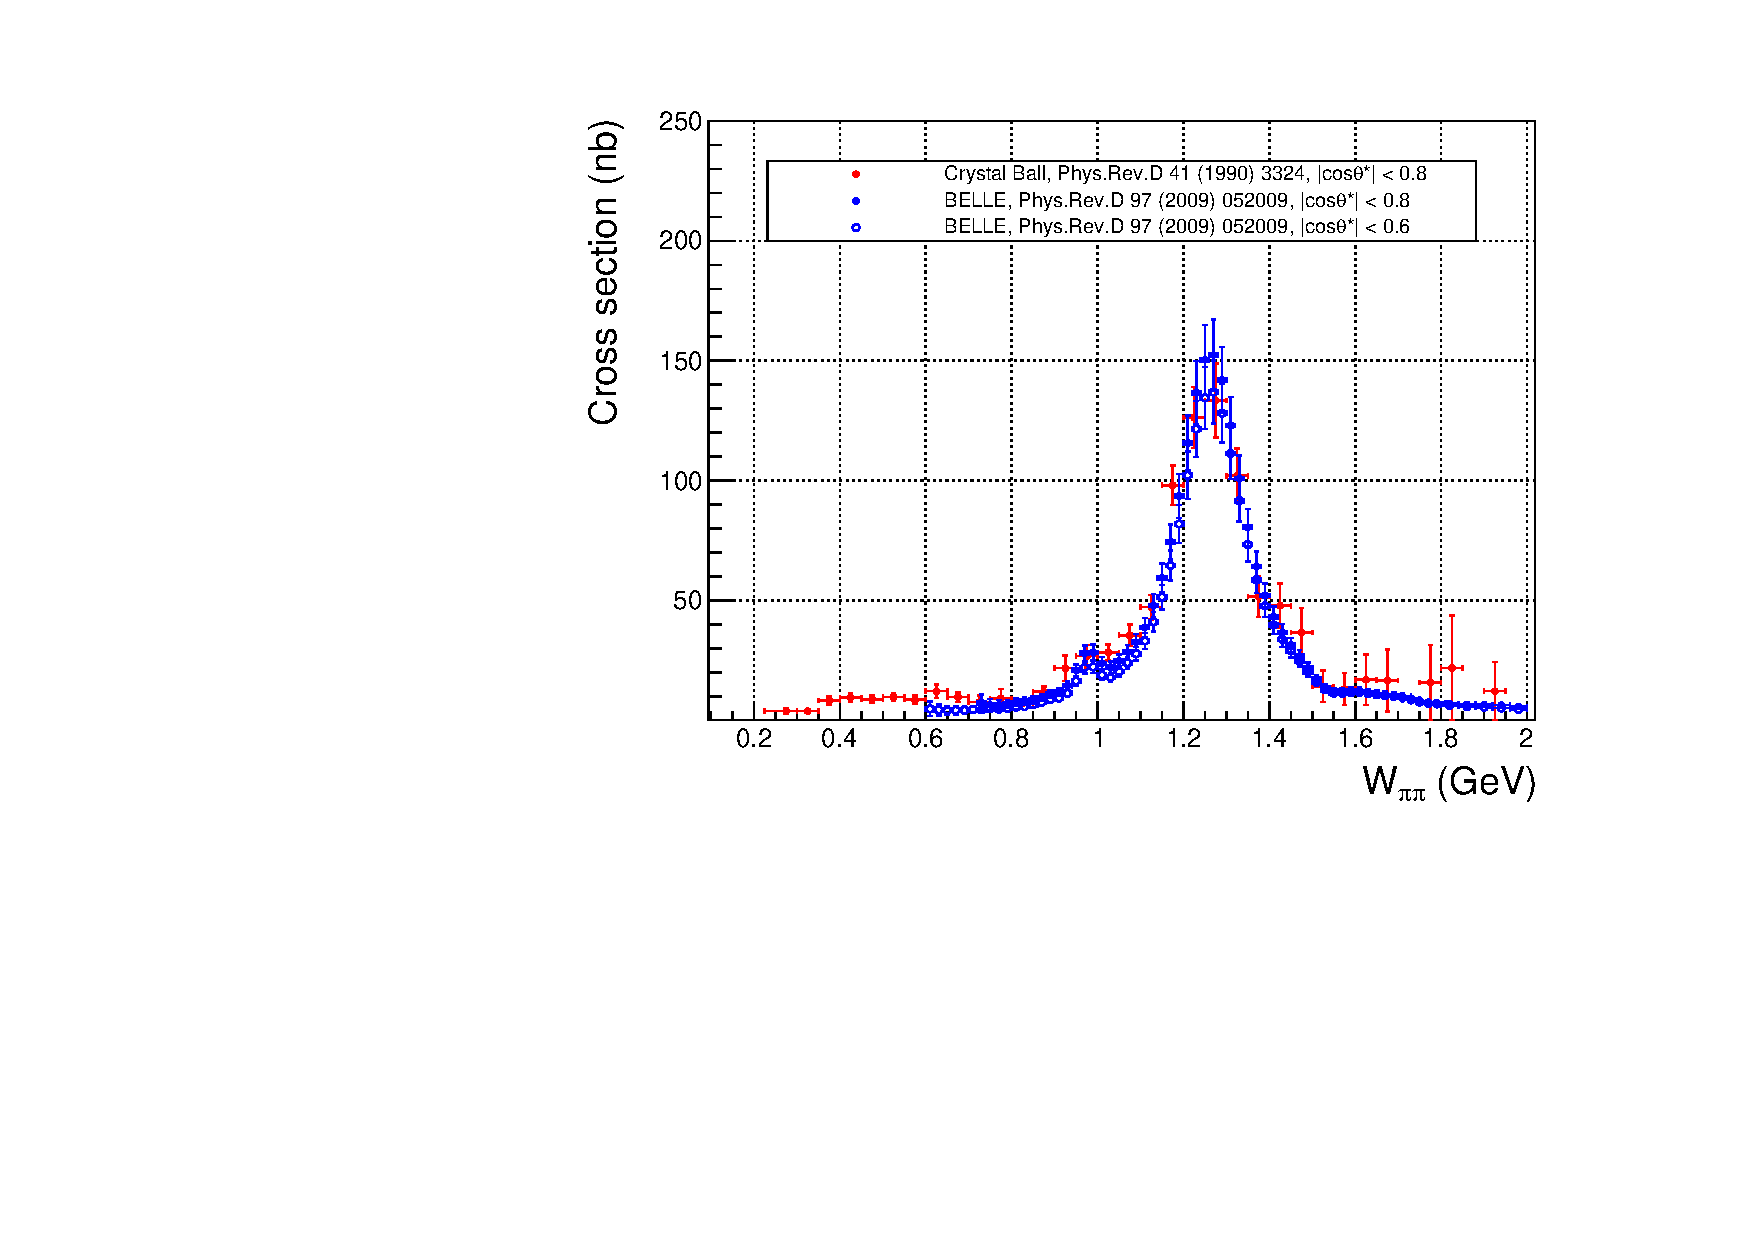
\includegraphics[height=5.5cm,angle=0]{figures/HEPData-ins815978-v1-Table_31_c2.pdf}
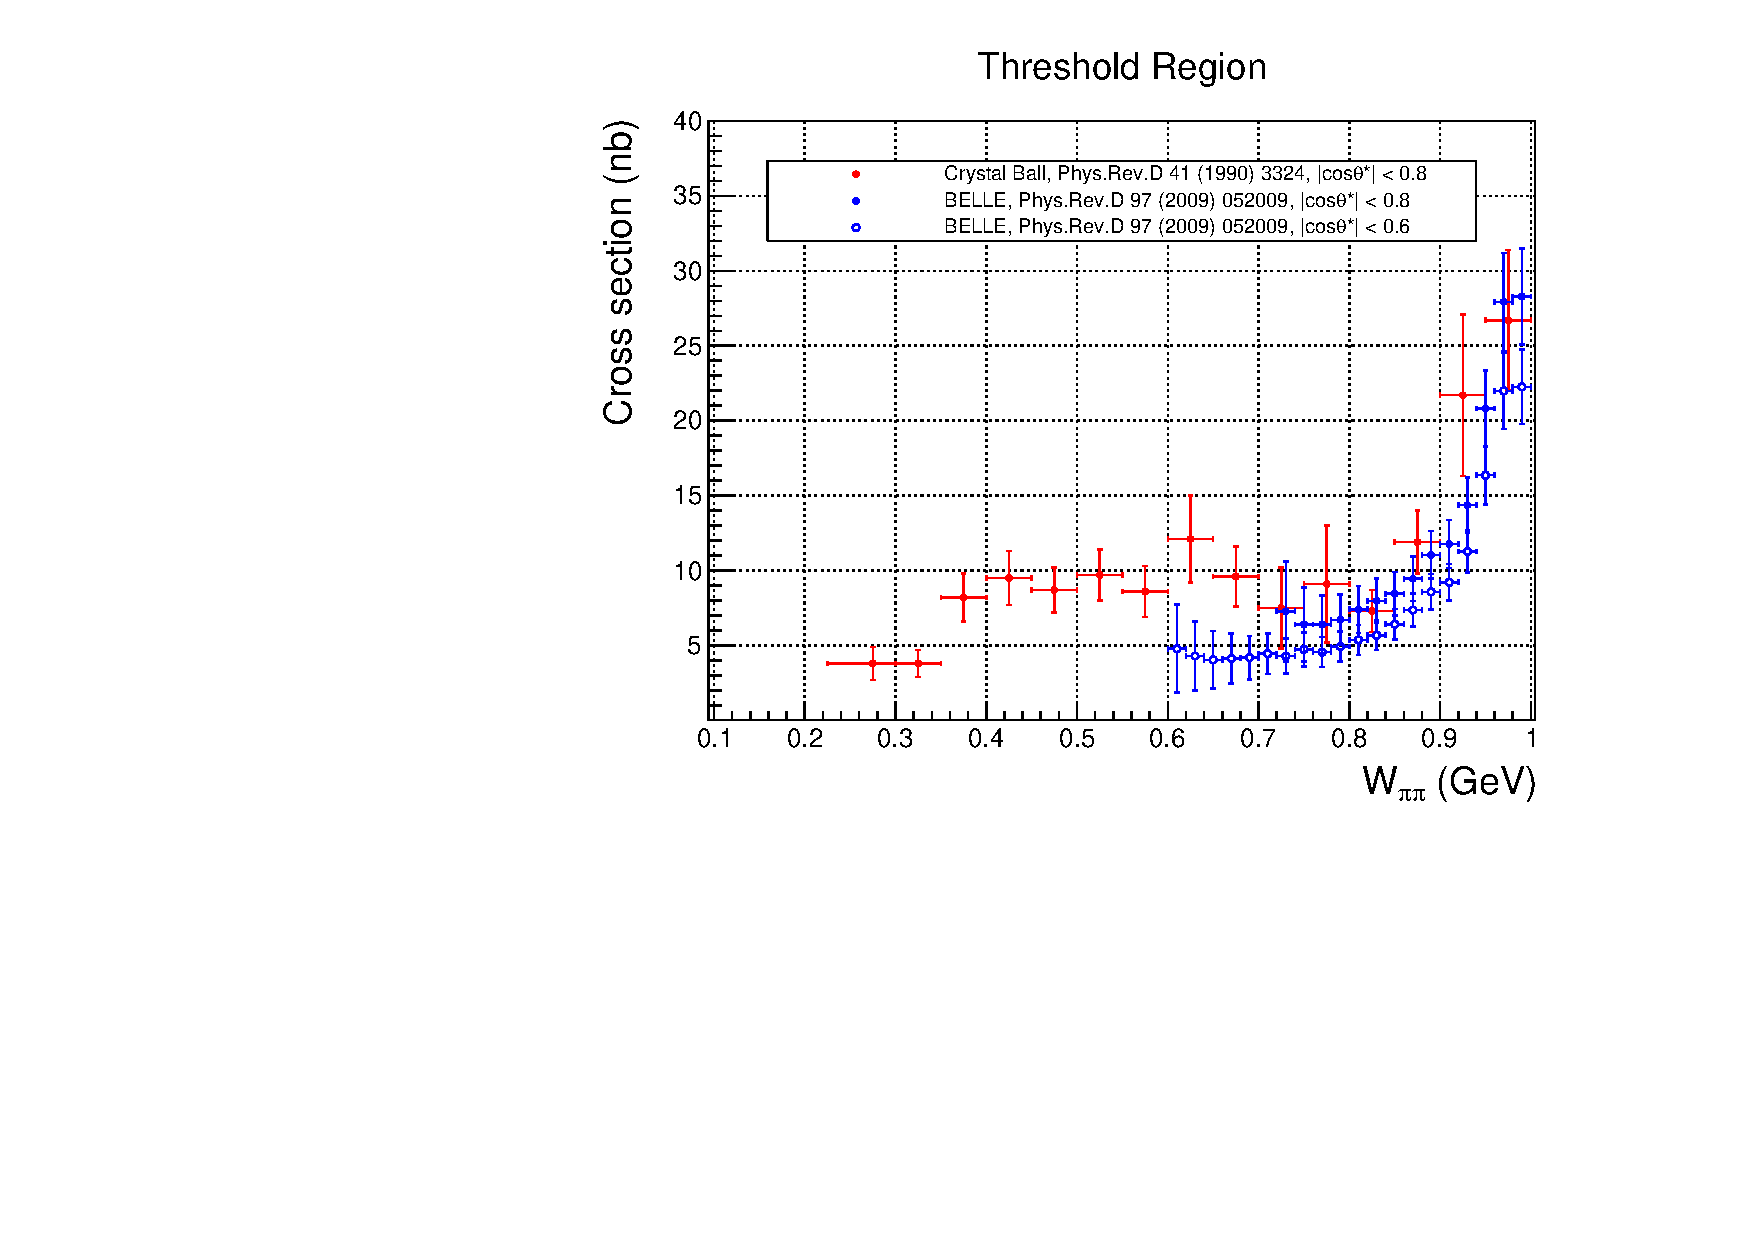
\includegraphics[height=5.5cm,angle=0]{figures/HEPData-ins815978-v1-Table_31_c1.pdf}
\end{center}
\caption{Data from Crystal Ball and BELLE. There are two data samples from BELLE experimental with different selection on $|\cos{\theta^*}|$. Left) Full range of $W_{\pi\pi}$. Right) Threshold region.
\label{fig:CrystalBall_BELLE_data}}
\end{figure}




%---------------------------------------------------------------------------------------------------------------
%---------Measurements of the charged  pion polarizability-------------------------------------
%---------------------------------------------------------------------------------------------------------------
%\input{PreviousMeasurements.tex}

%---------------------------------------------------------------------------------------------------------------
%---------Measurements of the charged  pion polarizability at Jefferson Lab Hall D-----
%---------------------------------------------------------------------------------------------------------------


 %<><><><><><><><><><><><><><><><><><><><><><><><><><><><><><><><><><><><><><><><><><><><><>
 % Experimental conditions
 %<><><><><><><><><><><><><><><><><><><><><><><><><><><><><><><><><><><><><><><><><><><><><>
\section{Experimental conditions}
The measurement of the neutral pion polarizability is expected to run
concurrently with the experiment to measure the charged pion
polarizability (CPP) \cite{CPPexp} in Hall D. Essentially all the
optimizations for that experiment are expected to improve the
sensitivity of this experiment also. We briefly summarize the
configuration for CPP, which is compared in
Table~\ref{tab:ccp_config} to nominal GlueX running.  
 
The diamond radiator will be adjusted to set the coherent peak of the
photon beam between 5.5 and 6.0~GeV. This enhances the polarization
significantly and also the tagging ratio compared to nominal GlueX conditions.
The experimental target
will be placed upstream of the nominal GlueX target by 64 cm (z=1\,cm
in the Hall D coordinate system). These changes benefit the present
experiment. In addition, the CPP experiment will add multi-wire
proportional chambers downstream for muon identification, but these do
not have an impact on this measurement.
 
% \begin{landscape}
\begin{table}[t]
\caption{Configuration of the CPP experiment compared to nominal GlueX. We propose that this experiment run concurrently with CPP. Detectors not identified
in the table are assumed to be operated under the same conditions as in the nominal configuration.
\label{tab:ccp_config}
}
\begin{center}
\begin{tabular}{|l|c|c|c|c|c|c|c|c|}
\hline
\hline 
  Configuration  & GlueX I  & CPP/NPP   \\  \hline \hline
  Electron  beam energy  &   11.6 GeV   &  11.6 GeV   \\ \hline 
  Emittance   &   10$^{-8}$m rad   &  10$^{-8}$m rad   \\ \hline 
  Electron  current  &   150 nA   &  20 nA  \\ \hline
  Radiator thickness  &   50$\mu$m  &  50 $\mu$m diamond   \\ \hline 
  Coherent peak  &   8.4 -- 9.0 GeV   &  5.5 -- 6.0 GeV     \\ \hline 
  Collimator aperture  &  5 mm & 5 mm   \\ \hline  
  Peak polarization  &   35\%   &  72\%     \\ \hline 
  % Coherent/Incoherent ratio  &  0.068   &   0.32?   \\ \hline  
  Tagging ratio  &   0.6   &   0.72 \\ \hline  
  Flux 5.5-6.0 GeV  &      &   11 MHz \\ \hline   
  Flux 8.4-9.0 GeV  &  20 MHz    &    \\ \hline  
  Flux 0.3-11.3 GeV  &  367 MHz    &   74 MHz \\ \hline 
  Target position  &   65 cm   &  1 cm    \\ \hline 
  Target, length   &  H, 30 cm   &  $^{208}$Pb, 0.028 cm   \\
%                            &   2.1 g/cm$^2$, 0.033 X$_0$ & 0.69 g/cm$^2$, 0.05 X$_0$ \\ 
 \hline  
  Start counter & nominal & removed \\ \hline
  Muon identification  &  None   &   Behind FCAL    \\ \hline   
  \hline
\end{tabular}
\end{center}
\end{table}
%\end{

\subsection{Expected signal}
In order to estimate rates, resolution and acceptance due to the
Primakoff reaction on lead, $\gamma ^{208}\rm{Pb}\rightarrow \pi^0
\pi^0\, \rm{Pb}$, we take the reaction process to be the same as for
charged pion production and given in Eq. 8 of the Proposal for the
Charged Pion Polarizability experiment \cite{CPPexp}, which is
reproduced here for convenience:
\begin{eqnarray}
\frac{d^2\sigma}{d\Omega_{\pi\pi}dW_{\pi\pi}} = \frac{2\alpha Z^2}{\pi^2} \frac{E^4_\gamma \beta^2}{W_{\pi\pi}} \frac{\sin^2\theta_{\pi\pi}}{Q^4} |F(Q^2)|^2 \sigma(\gamma\gamma\rightarrow\pi^0\pi^0) (1+P_\gamma \cos{2\phi_{\pi\pi}}).   \label{eq:PrimakoffSignal}
\end{eqnarray}
The $\gamma\gamma$ cross section for charged pions has been
substituted with the cross section for neutral pions, namely
$\sigma(\gamma\gamma\rightarrow\pi^0\pi^0)$. In this expression,
$\Omega_{\pi\pi}$ is the solid angle in the laboratory frame for the
emission of the $\pi\pi$ system, $W_{\pi\pi}$ is the $\pi\pi$
invariant mass, Z is the atomic number of the target, $\beta$ is the
velocity of the $\pi\pi$ system, $E_\gamma$ is the energy of the
incident photon, $F(Q^2)$ is the electromagnetic form factor for the
target with final-state-interactions (FSI) corrections applied,https://www.overleaf.com/project/5d5d22c3f2f2fe72b728c4e6
$\theta_{\pi\pi}$ is the lab angle for the $\pi\pi$ system,
$\phi_{\pi\pi}$ is the azimuthal angle of the $\pi\pi$ system relative
to the incident photon polarization, and $P_\gamma$ is the incident
photon polarization.\footnote{The expression for the cross section in
  terms of invariant quantities can be found in
  Ref.\,\cite{hdnote3186}.}
\begin{figure}[tph]
\centering
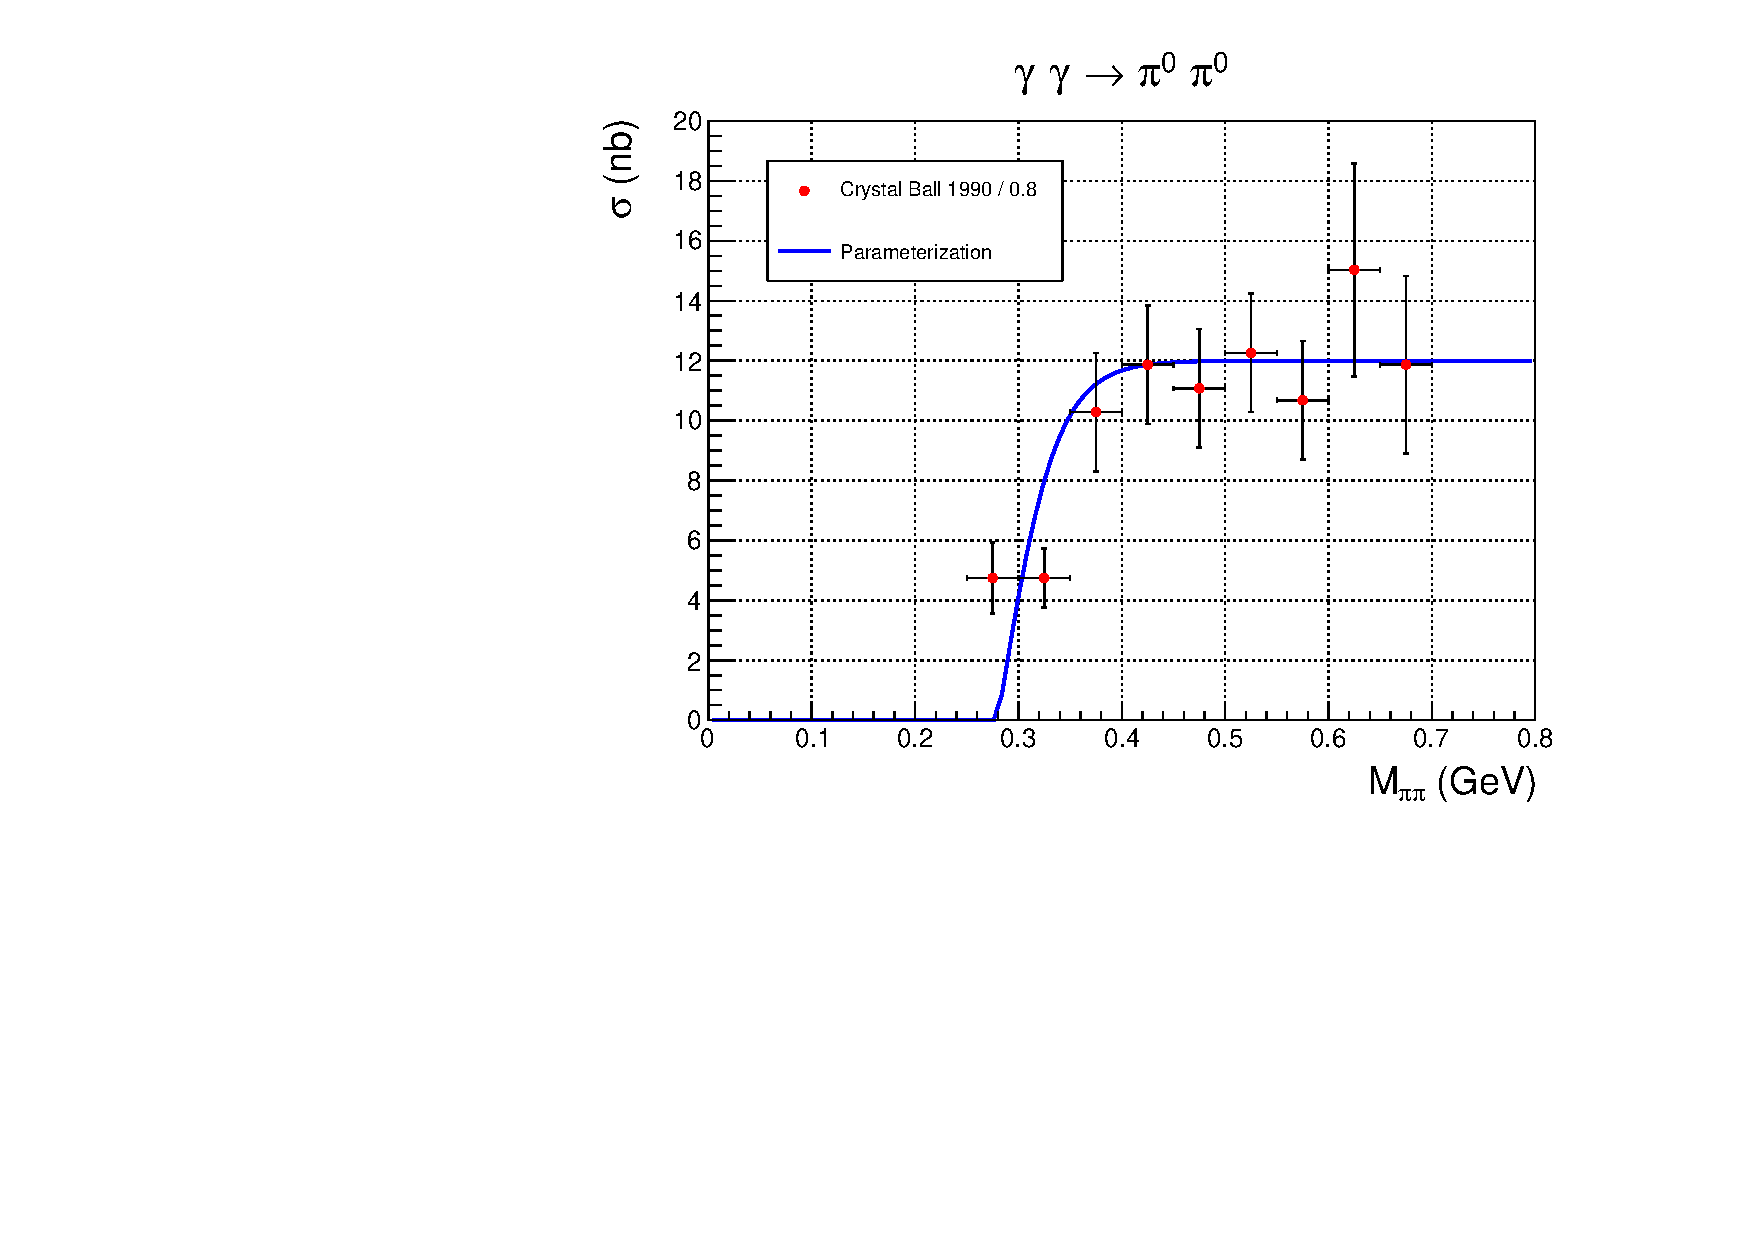
\includegraphics[page=1,width=4.75in]{figures/sigma_2pi0_figs.pdf}
\caption{Parameterization of the $\sigma(\gamma\gamma\rightarrow \pi^0\pi^0)$ cross section as a function
of the 2$\pi$ invariant mass compared to the data from Crystal Ball \cite{Marsiske:1990hx}.
\label{fig:sigma_2pi0_figs_1}}
\end{figure}

The cross section for $\sigma(\gamma\gamma\rightarrow\pi^0\pi^0)$ has
been measured by the Crystal Ball Collaboration
\cite{Marsiske:1990hx}, albeit with limited statistical precision. We
have parameterized the cross section for $W_{\pi\pi}<0.8$ GeV, which
is of specific interest to this program as shown in
Fig.\ref{fig:sigma_2pi0_figs_1}. Using this parameterization and
Eq.\ref{eq:PrimakoffSignal}, we can calculate the photoproduction
cross section on lead, which is shown in
Fig.\ref{fig:sigma_2pi0_figs_2}.
\begin{figure}[tph]
\centering
\includegraphics[page=2,width=4.75in]{figures/sigma_2pi0_figs.pdf}
\caption{Primakoff cross section for $\gamma Pb \rightarrow Pb\, \pi^0 \pi^0$ using the parameterization of  $\sigma(\gamma\gamma\rightarrow \pi^0\pi^0)$ in the previous figure. The integrated cross section is 0.3\,$\mu$b/nucleus.
\label{fig:sigma_2pi0_figs_2}}
\end{figure}
The integrated cross section is 0.30\,$\pm0.05\mu$b/nucleus. The uncertainty comes from the model dependence and was obtained by comparing two different calculations using completely different parameterizations for the nuclear form factor on lead, $F(Q^2)$. For reference,
we note that the cross section for charged pions $(\pi^+\pi^-$)
production is 10.9\,$\mu$b, a factor of 30 larger.

The number of neutral-pion-Primakoff-signal events produced during 20
PAC days is shown in Fig.\ref{fig:sigma_2pi0_figs_3}. The impacts of
detector trigger, acceptance and resolution are discussed in the next
section.
\begin{figure}[tph]
\centering
\includegraphics[page=3,width=4.75in]{figures/sigma_2pi0_figs.pdf}
\caption{Estimated production rate  for $\gamma \rm{Pb}\rightarrow \pi^0\pi^0\,\rm{Pb}$ as a function 2$\pi$ mass. For this calculation, it is assumed the detector has perfect resolution and has a linearly increasing efficiency from zero at threshold up to 0.4 at 0.34 GeV (see top right of Fig.\,\ref{fig:twopi_primakoff_DSelect_p1_W_100000_sum} ).
\label{fig:sigma_2pi0_figs_3}}
\end{figure}

\subsection{Detector resolution}
\label{sec:acceptance}
The response of the GlueX detector to neutral pion Primakoff events
was simulated using the standard GlueX generation and reconstruction
tools, but with the specific geometry for the CPP experiment. The schematic of the detector configuration is shown in
Fig.\,\ref{fig:GlueX_cpp}. The primary differences between the
standard GlueX geometry and CPP are summarized in
Table\,\ref{tab:ccp_config}. For this experiment, the main differences
include a) coherent peak position at 5.5-6 GeV and re-positioning of
the microscope to cover the coherent peak, b) solid $^{208}$Pb at
z=1cm, and c) Start counter removed. For the CPP experiment, the
addition of muon identification chambers behind the FCAL is
critical. However, for neutral pions this addition plays no role
because the photons are detected in the FCAL. The GEANT4 simulation,\footnote{The initial simulations used GEANT3
and show similar results.}
which is used for these studies, includes most changes except for the
addition of the muon chambers, which are not needed. In addition, the
microscope geometry has not been modified and we use the tagger
hodoscope for that region in the simulation. The slightly reduced
energy of the hodoscope relative to the microscope has little impact
and the gaps between counters is ignored by simulating the tagged
flux.
\begin{figure}[h!]
\centering
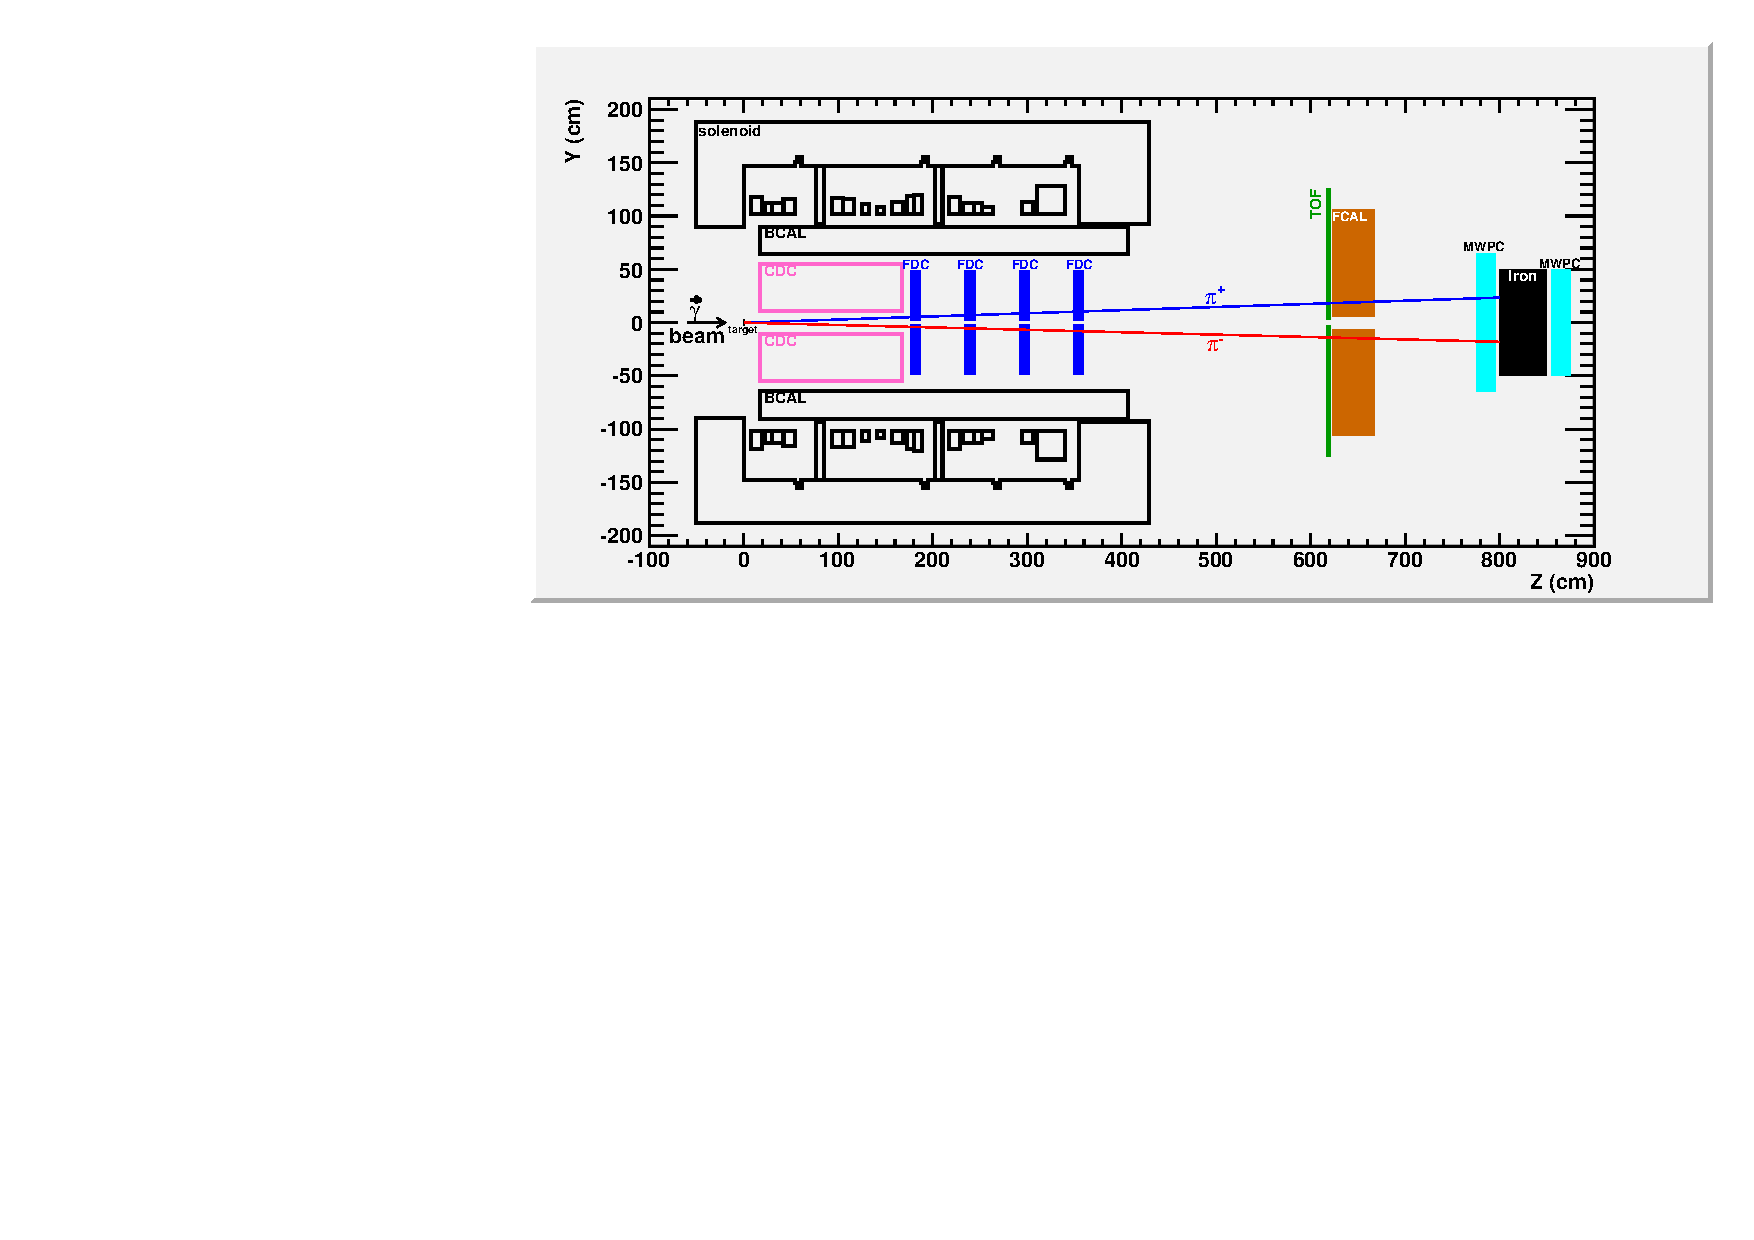
\includegraphics[width=5.25in]{figures/GlueX_cpp.pdf}
\caption{Diagram of the GlueX detector including the additional muon chambers for the CPP experiment.}
\label{fig:GlueX_cpp}
\end{figure}

The Primakoff signal was generated according to the cross section
described in the previous chapter, using the
\emph{gen\_2pi0\_primakoff}, which is a modified version of the CPP event generator. By default, the production amplitudes are
symmetrized between the two identical $\pi^0$'s by AmpTools. One
hundred thousand events of Primakoff and nuclear coherent interactions 
(see Section\,\ref{sec:NCback}) were generated with $M_{\pi\pi}<$0.9 GeV.
We used random triggers from run 30401\footnote{Run 30401 is a low-intensity run for GlueX,
but represents considerably higher background than expected for this experiment.} to add tagger accidentals 
and random hits in the drift chambers. These events were fed to GEANT4 to track particles, and subsequently
processed using \emph{mcsmear} to simulate the detector response. The
simulated events were then analyzed using the GlueX event filter to
analyze the reaction $\gamma Pb \rightarrow \pi^0 \pi^0$ with a
missing Pb nucleus and constraining the detected photon pairs to the
$\pi^0$ mass. Energy and momentum conservation is imposed on the reaction as well as the requirement that all photons originate from a common vertex (i.e. ``vertex-P4''). The output of the reconstruction, both kinematically
fit and ``measured" quantities, were available for inspection.

In the following we show various reconstructed quantities as well as
estimated resolutions. The distribution of generated photon energy and
the unconstrained reconstructed momenta of the two pions are shown in
Fig.\,\ref{fig:EgP1P2_signal_DSelector}.
\begin{figure}[tph]
\centering
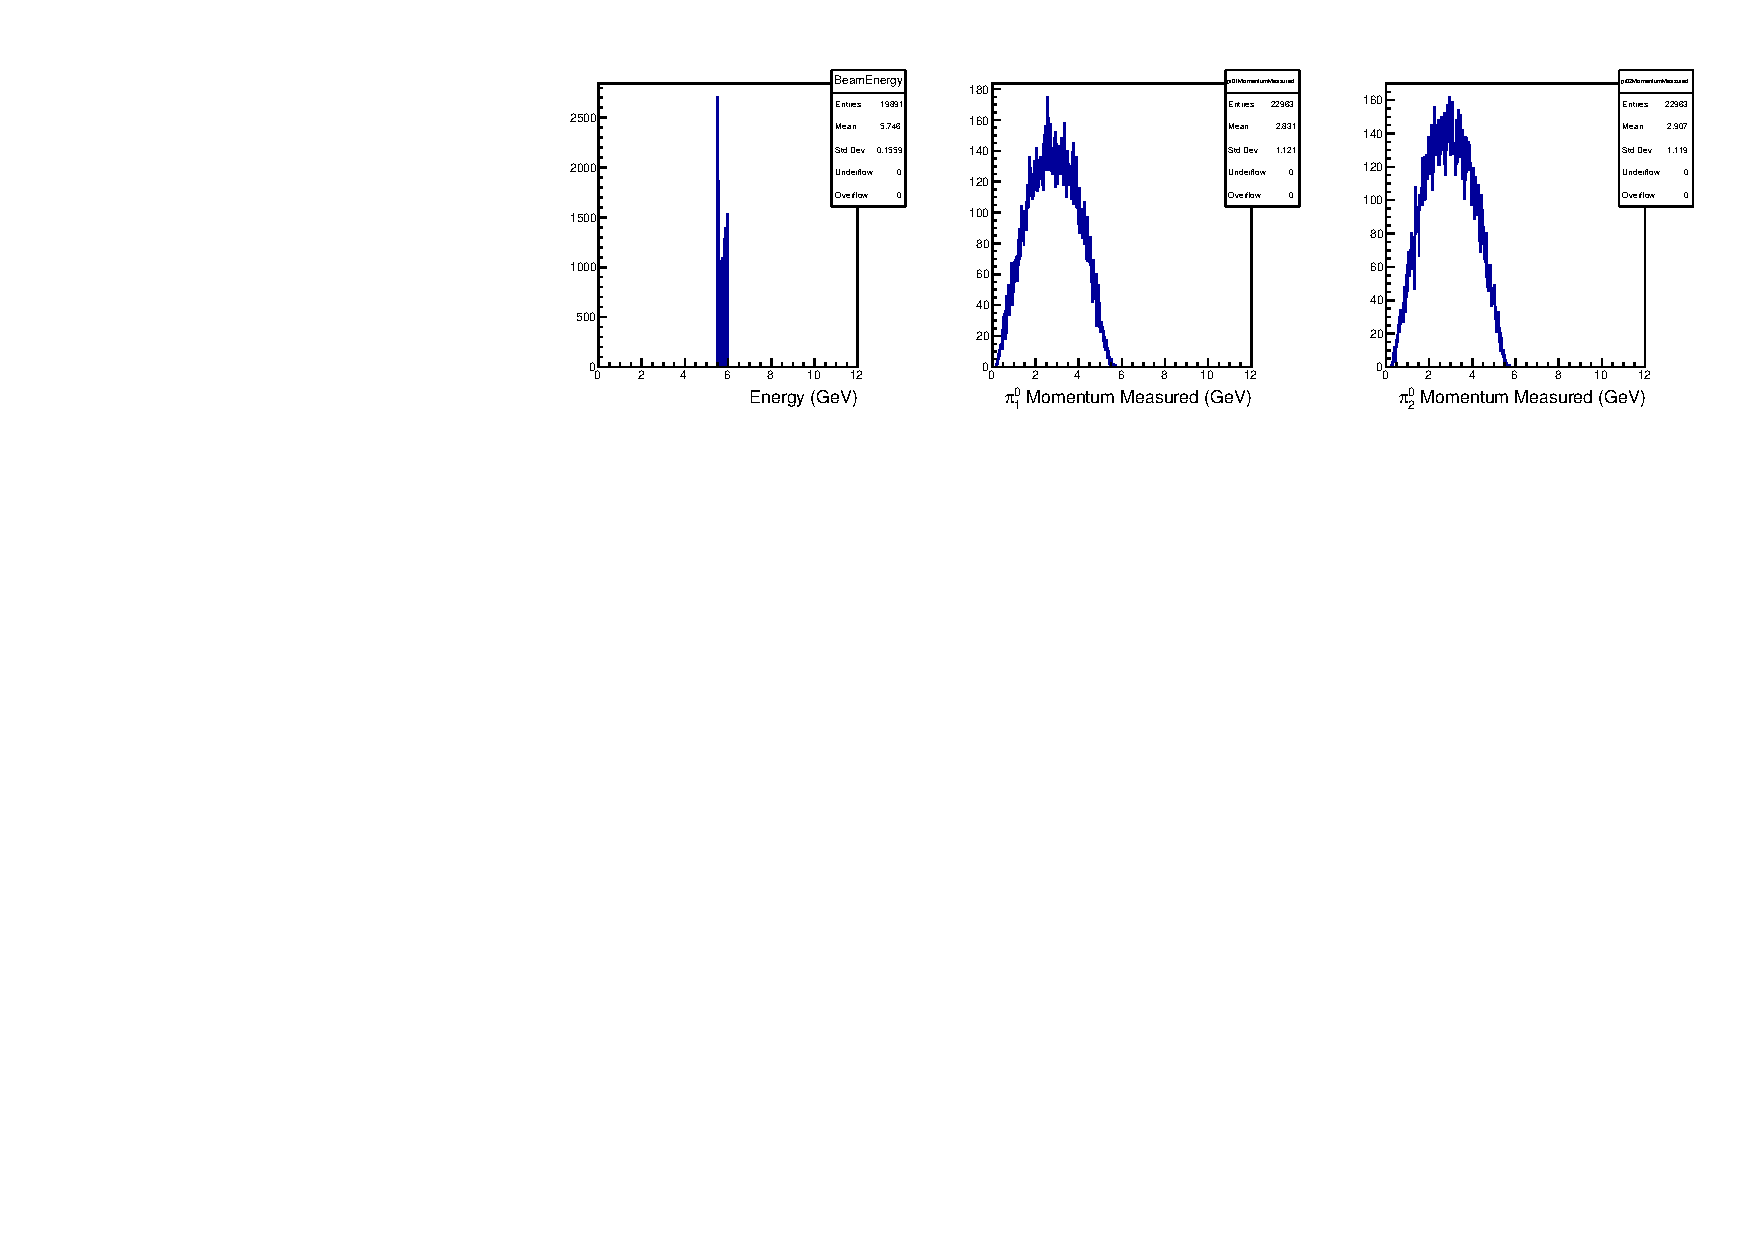
\includegraphics[width=6in]{figures/EgP1P2_signal_DSelector.pdf}
\caption{Left: Generated photon energies. The increased rate near 5.5 GeV is due to tagger accidentals. Center: Reconstructed momentum distribution of one $\pi^0$. Right: Reconstructed momentum distribution of the second $\pi^0$.
\label{fig:EgP1P2_signal_DSelector}}
\end{figure}
The missing mass, 2$\pi$ mass and $-t$ distributions are shown in Fig.\,\ref{fig:MMMpipit_signal_DSelector}.
\begin{figure}[tph]
\centering
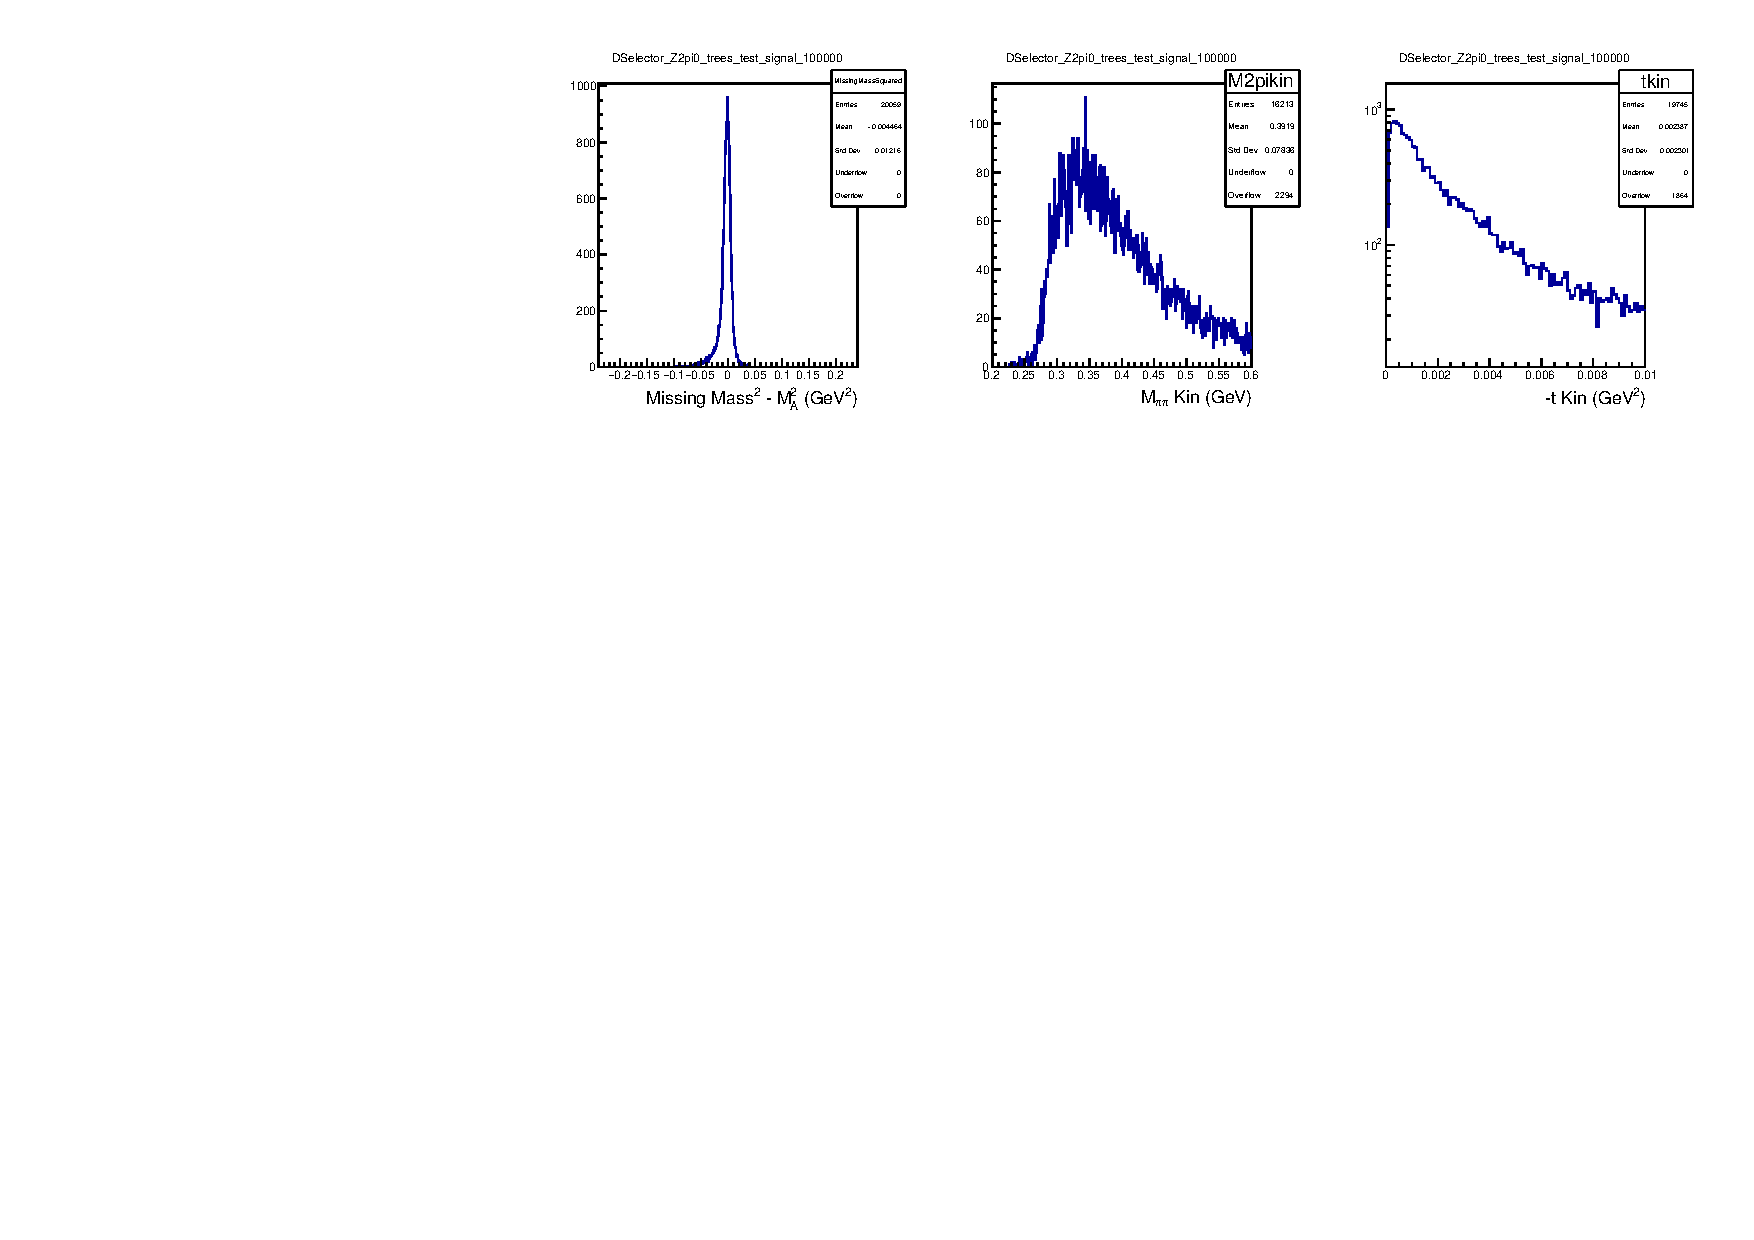
\includegraphics[width=6in]{figures/MMMpipit_signal_DSelector.pdf}
\caption{Left: Missing mass distribution minus the mass of the recoil nucleus. Center: Kinematically fit $2\pi$ mass distribution. Right: Kinematically fit -t distribution.
\label{fig:MMMpipit_signal_DSelector}}
\end{figure}
The reconstructed momentum relative to its generated value is shown in
Fig.\ref{fig:DeltapDeltaPhi_signal_DSelector}. The central peak of the
kinematicall fit momentum is about 2\%, similar to that for charged
pions. However, there are long uniform tails that will effect the
final reconstruction. The resolution of the azimuthal angle,
$\phi_{\pi\pi}$, between the production and the photon polarization
planes is quite poor owing to the fact that the pion pairs are
produced at very shallow angles. Nevertheless it is sufficient to
measure the asymmetry due to the photon beam polarization.
\begin{figure}[tph]
\centering
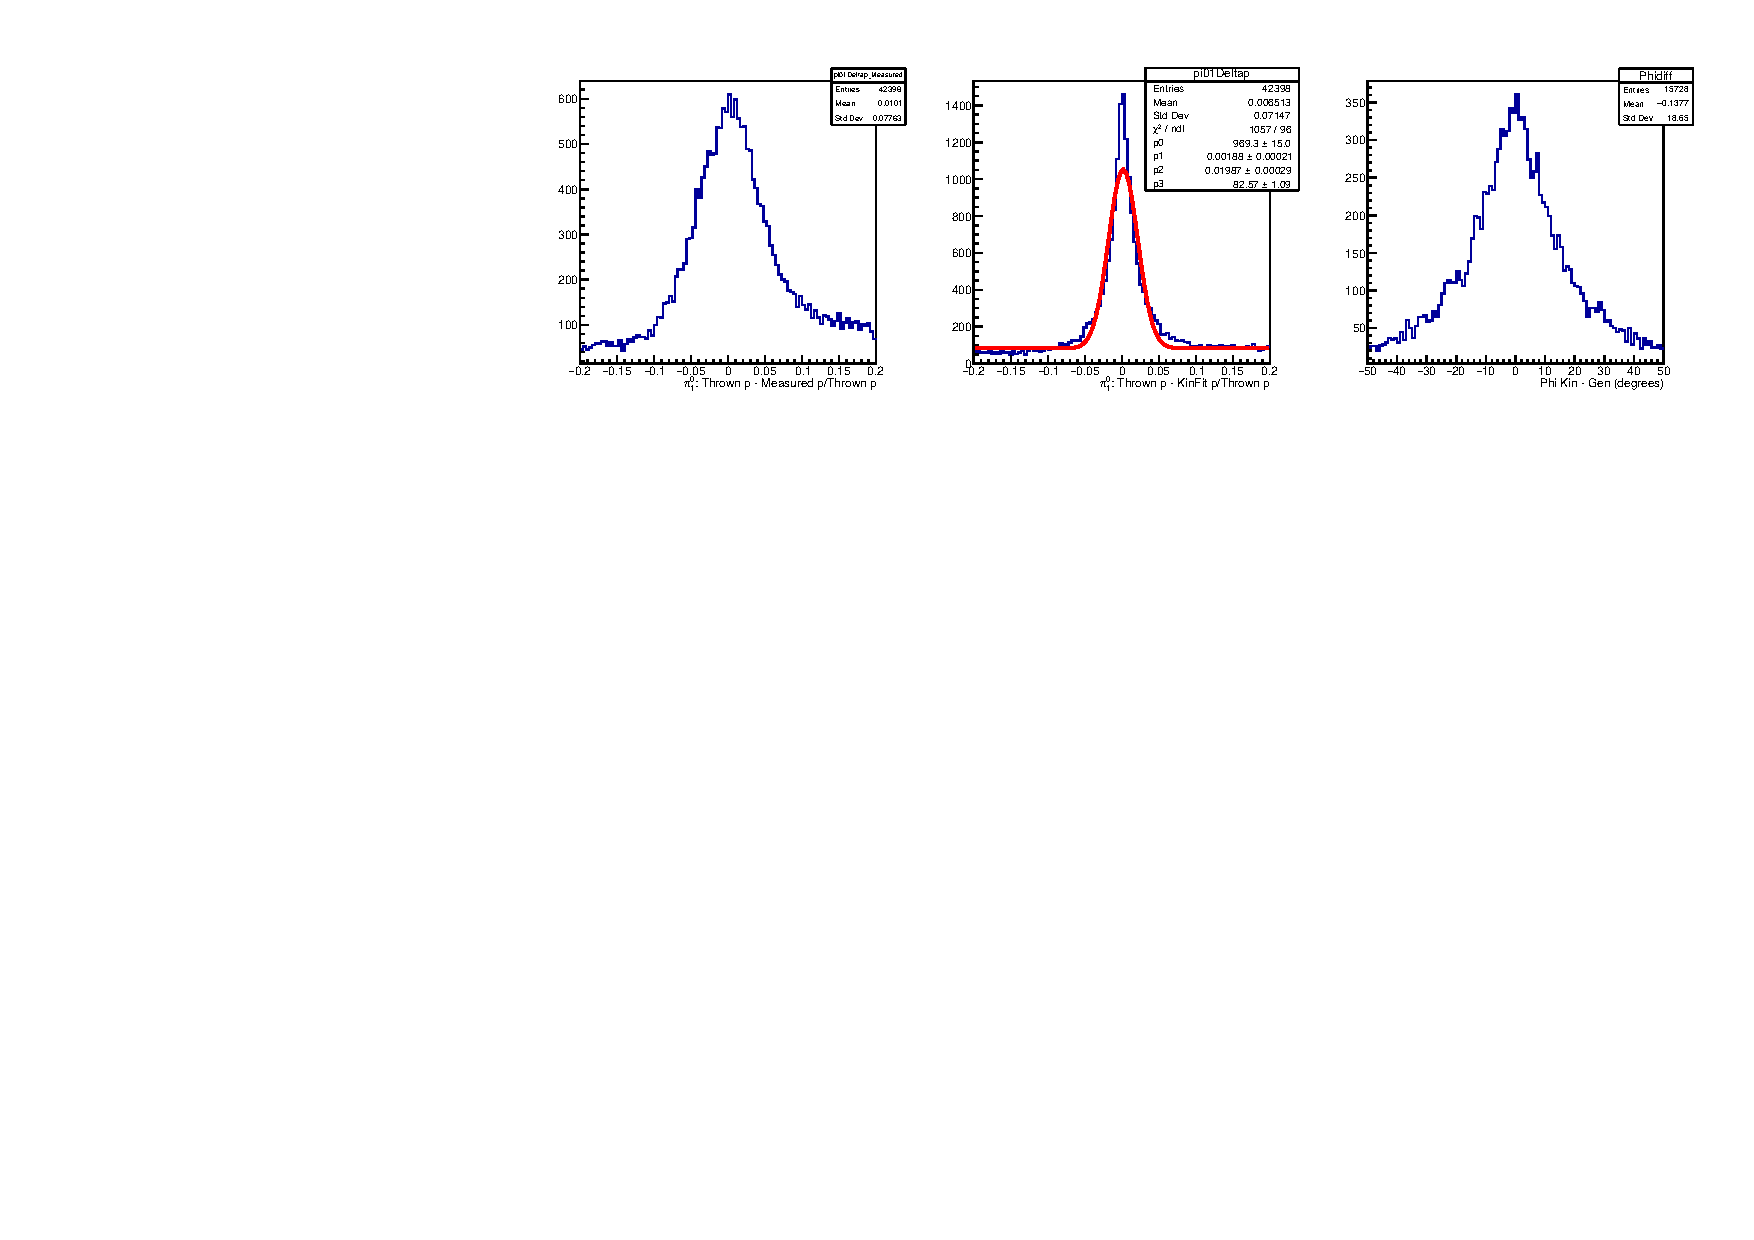
\includegraphics[width=6in]{figures/DeltapDeltaPhi_signal_DSelector.pdf}
\caption{Left: Difference between measured and generated momentum. Center: Difference between kinematically fit and generated momentum. The central peak has a width of about 2\%. Right: Difference between the kinematically fit azimuthal angle $\phi_{\pi\pi}$ and its generated value.
\label{fig:DeltapDeltaPhi_signal_DSelector}}
\end{figure}
The resolution of the 2$\pi$ invariant mass is shown in Fig.\,\ref{fig:Resolution_Mpipittag_signal_DSelector}, along with the resolution of Mandelstam $-t$, and the reconstructed time resolution. The mass resolution is about 12\,MeV.
\begin{figure}[tph]
\centering
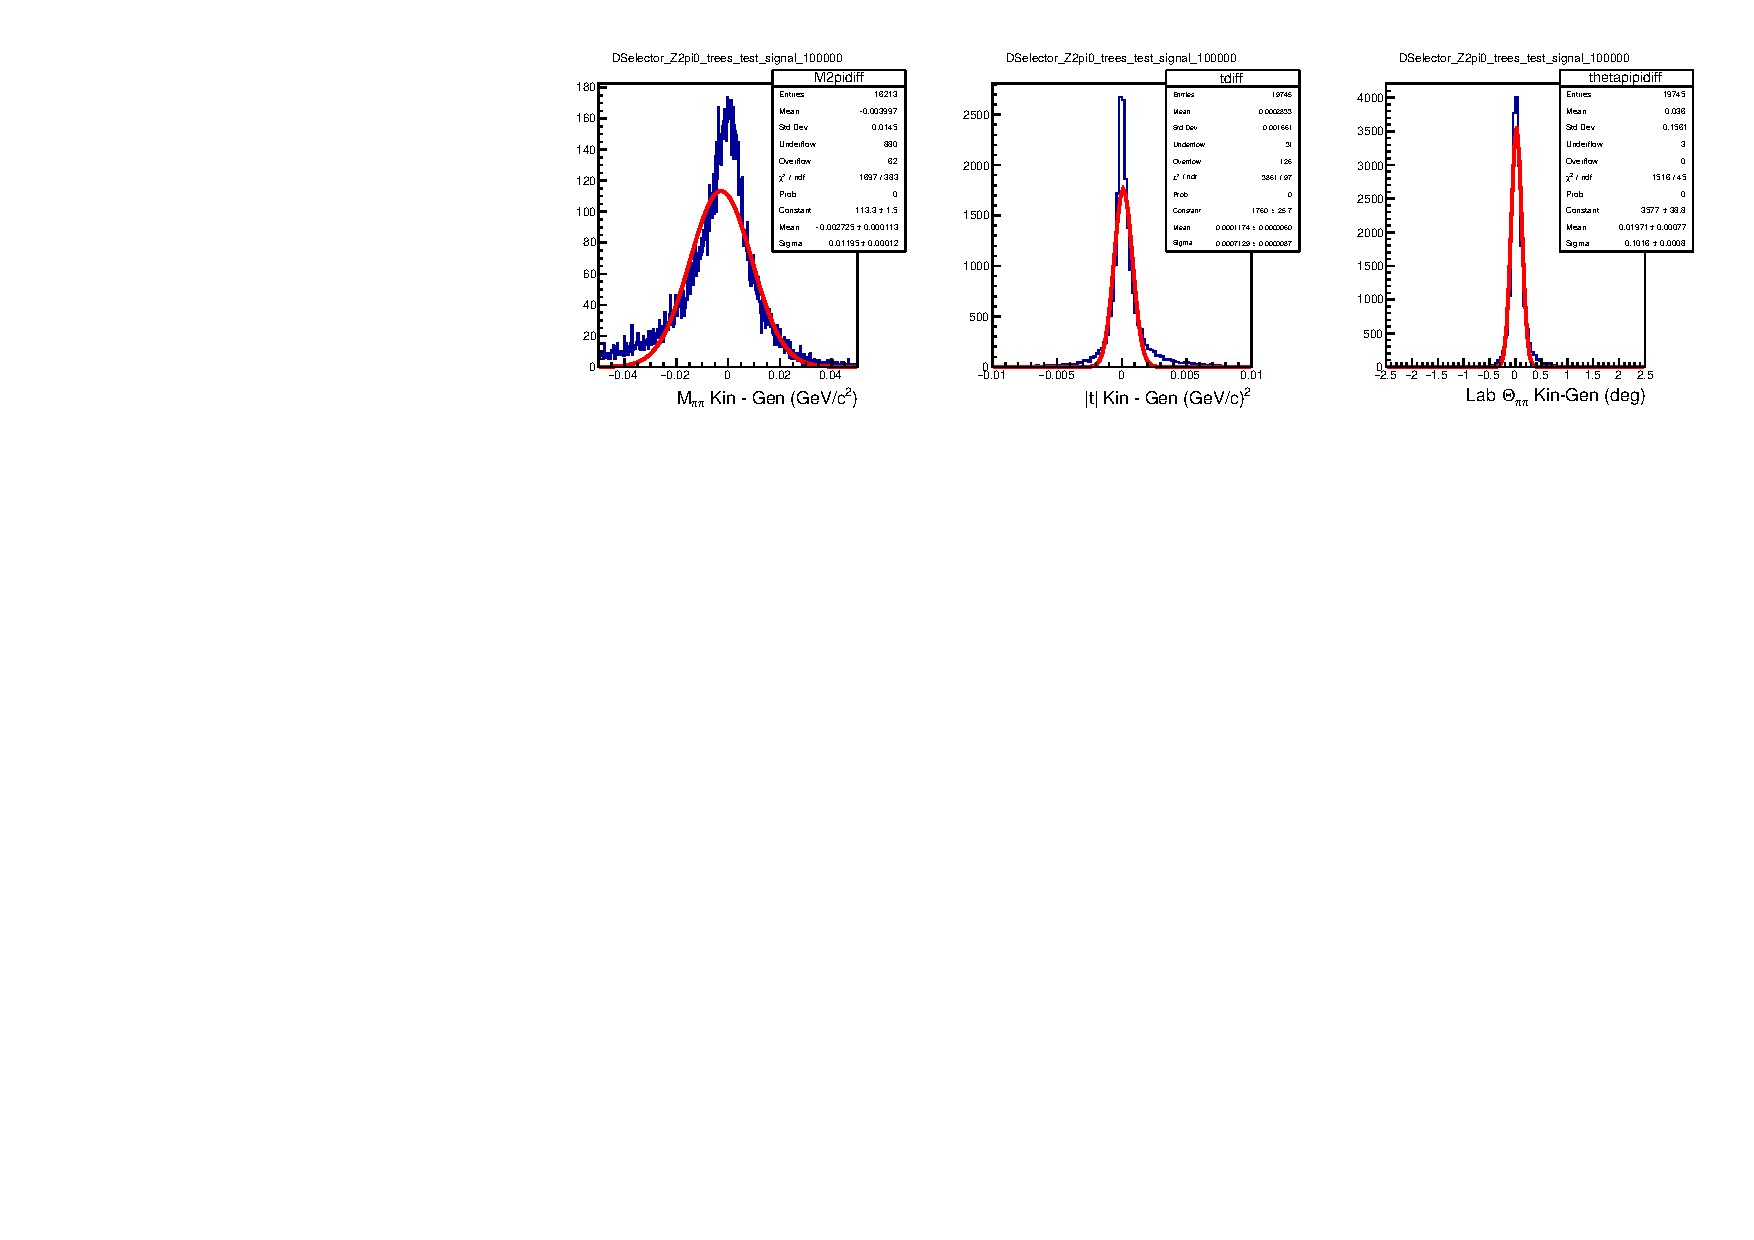
\includegraphics[width=6in]{figures/Resolution_Mpipittag_signal_DSelector.pdf}
\caption{Left: Difference between kinematically fit and generated 2$\pi$ mass. The central 2$\pi$-mass $\sigma$ is about 12 MeV. Center: Difference between kinematically fit and generated -t. Right: Difference between kinematically fit and generated 2$\pi$ polar angle. The resolution $\sigma$ of the reconstructed angle is 0.1 degrees.
%Right: Timing resolution relative to the accelerator RF signal is about 0.35 ns.
\label{fig:Resolution_Mpipittag_signal_DSelector}}
\end{figure}

\subsection{Trigger and acceptance}
The Primakoff reaction will transfer all the energy of the beam into
four photons, which are going forward. All this energy will be
deposited in the FCAL, except for leakage down the beampipe. We expect
a simple trigger with an energy threshold in the FCAL should have very
high efficiency for any events that can be reconstructed:
the FCAL trigger with the total energy threshold around 1$\,$GeV can be used. To estimate trigger rate we used the same method as for TOF trigger rate \cite{TOFrate} extracted from the dedicated runs with high random trigger frequency. We used FCAL total energy greater than 1GeV deposited within 40$\,$ns excluding the most inner FCAL layer as a trigger condition. Fig.~\ref{fig:fcalrate} shows the values for LH2 and ''empty'' target configurations.
Since the proposed lead target is 1.7 times thicker than LH2 target (in rad. lengths), we used ''empty'' target rate plus the difference between LH2 and ''empty'' target rates scaled with the factor of 1.7. That gives the value $\sim$9$\,$kHz for 20$\,$nA beam current.

\begin{figure}[tph]
\centering
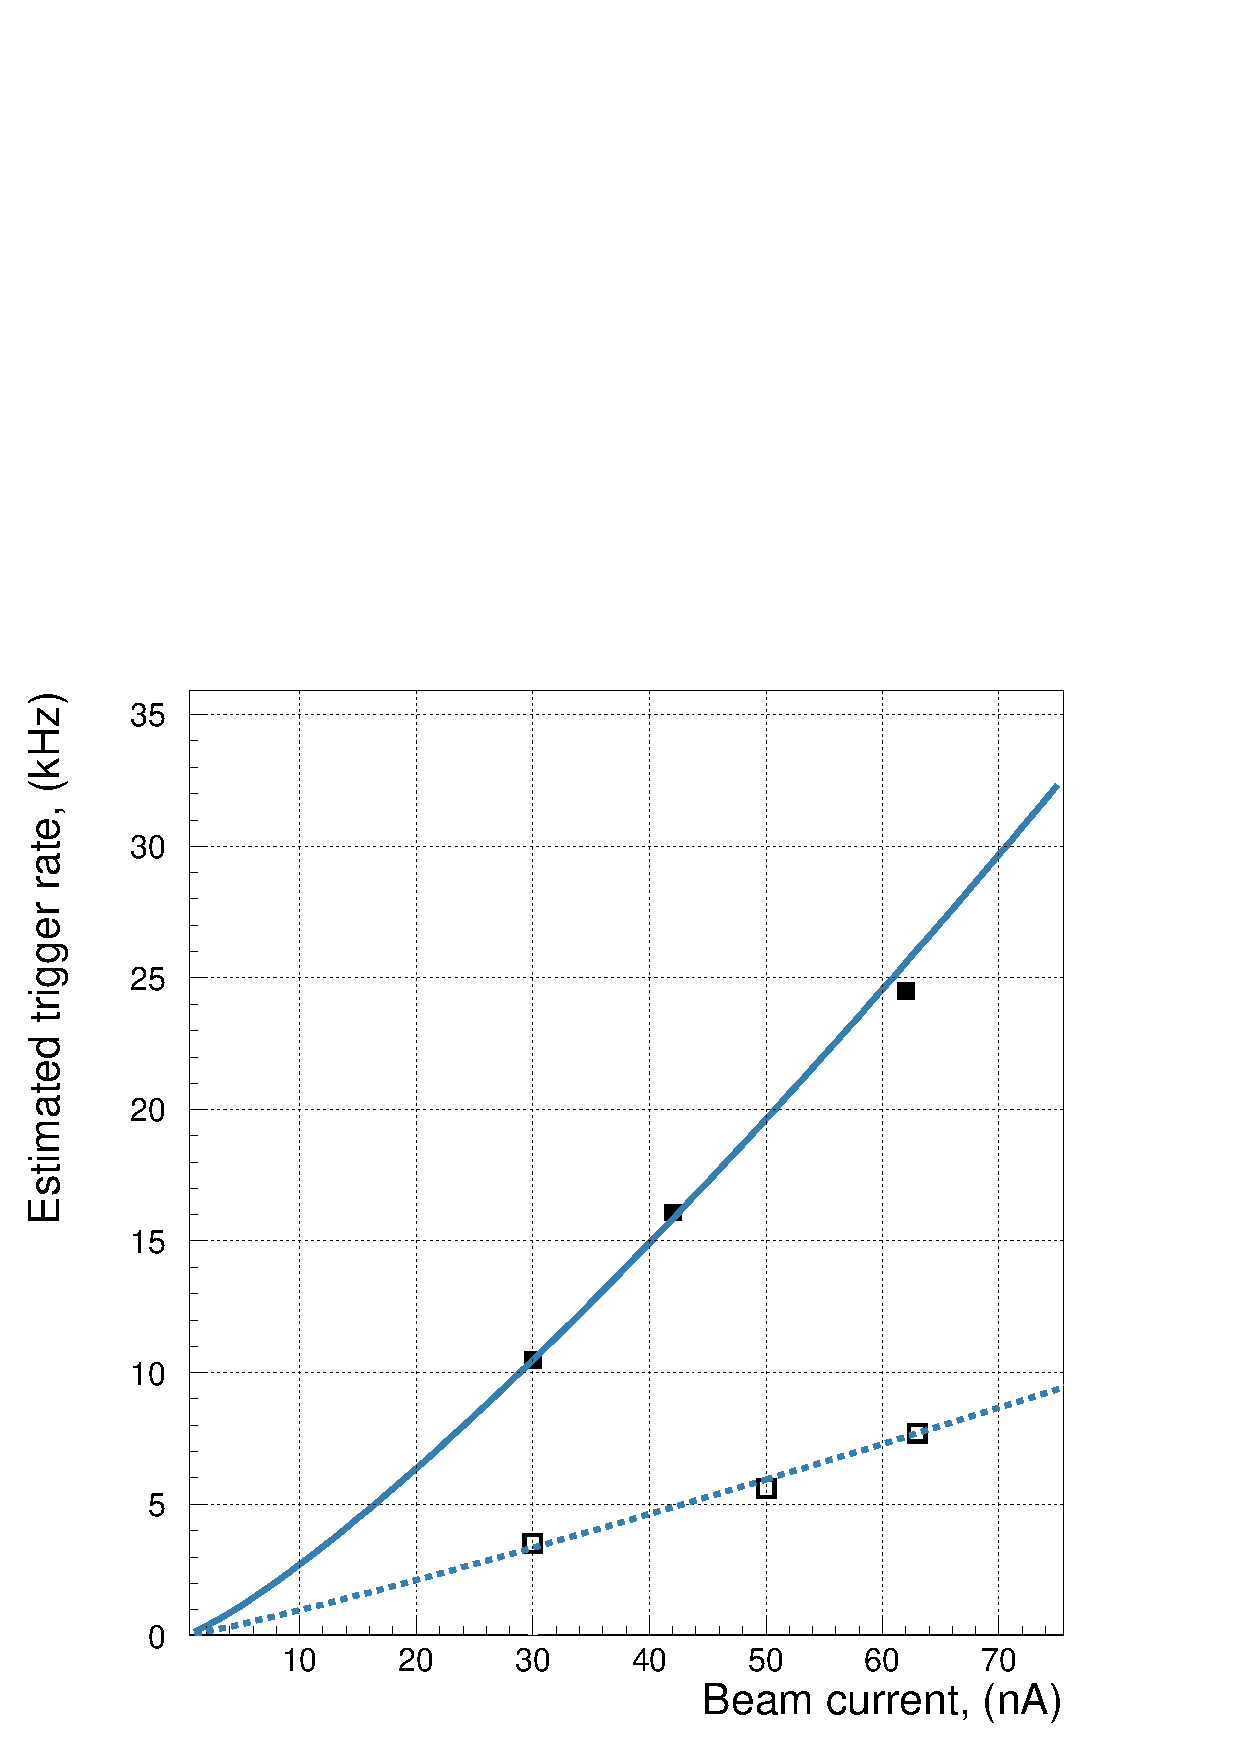
\includegraphics[width=3in]{figures/fcalrate_vs_beam.pdf}
\caption{Estimated FCAL trigger rate for 1$\,$GeV
total energy threshold for LH2 (solid squares) and ''empty'' (empty squares) targets.
\label{fig:fcalrate}}
\end{figure}





The acceptance of the signal events can be determined by comparing the
kinematically fit to the generated distributions. The generated and
kinematically fit 2$\pi$ mass, $\phi_{\pi\pi}$ and $-t$ distributions
are shown in
Fig.\,\ref{fig:twopi_primakoff_DSelect_p1_W_100000_sum}. The
reconstruction was described in the previous section.
\begin{figure}[tph]
\centering
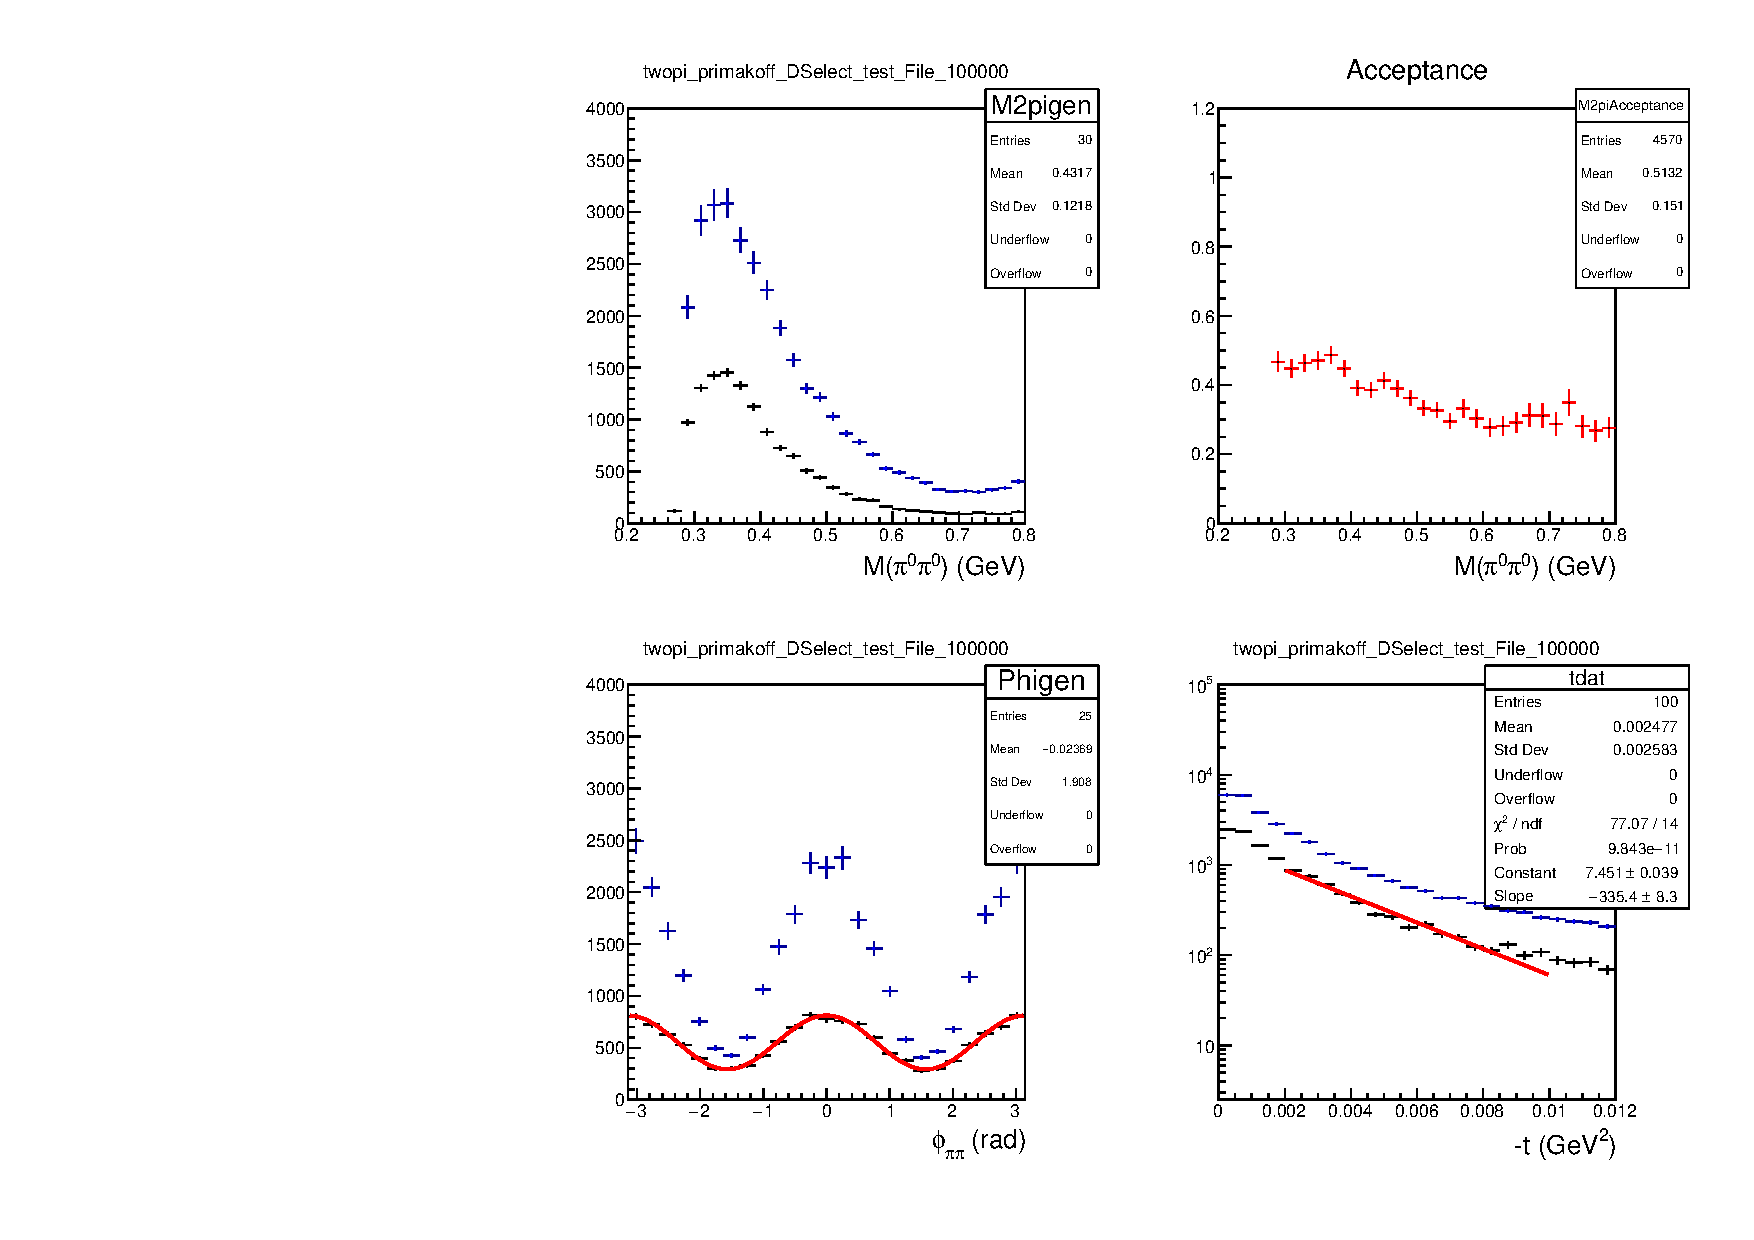
\includegraphics[width=6in]{figures/twopi_primakoff_DSelect_test_File_100000_sum_PrimNC.pdf}
\caption{Top left: Generated and kinematically fit (accepted) 2$\pi$-mass distribution. Top right: Acceptance as a function of 2$\pi$ mass. The acceptance is about 40\% at threshold. Bottom left: Generated and kinematically fit azimuthal angle $\phi_{\pi\pi}$. Bottom right: Generated and kinematically fit $-t$ distribution. }
\label{fig:twopi_primakoff_DSelect_p1_W_100000_sum}
\end{figure}
The acceptance is quite high at about 40\%. However, there is also
significant slewing due to resolution in most variables of
interest.  The
relatively poor resolution in $\phi_{\pi\pi}$ results in dilution of
the measured azimuthal dependence, which will need to be adjusted
based on simulation. Finally the measured $-t$ resolution roughly reproduces the generated slope despite the smearing of high rate regions down to low rate
regions.


%<><><><><><><><><><><><><><><><><><><><><><><><><><><><><><><><><><><><><><><><><><><><><>
 % Backgrounds
 %<><><><><><><><><><><><><><><><><><><><><><><><><><><><><><><><><><><><><><><><><><><><><>
\section{Backgrounds}

\begin{figure}[tbp]
\begin{center}
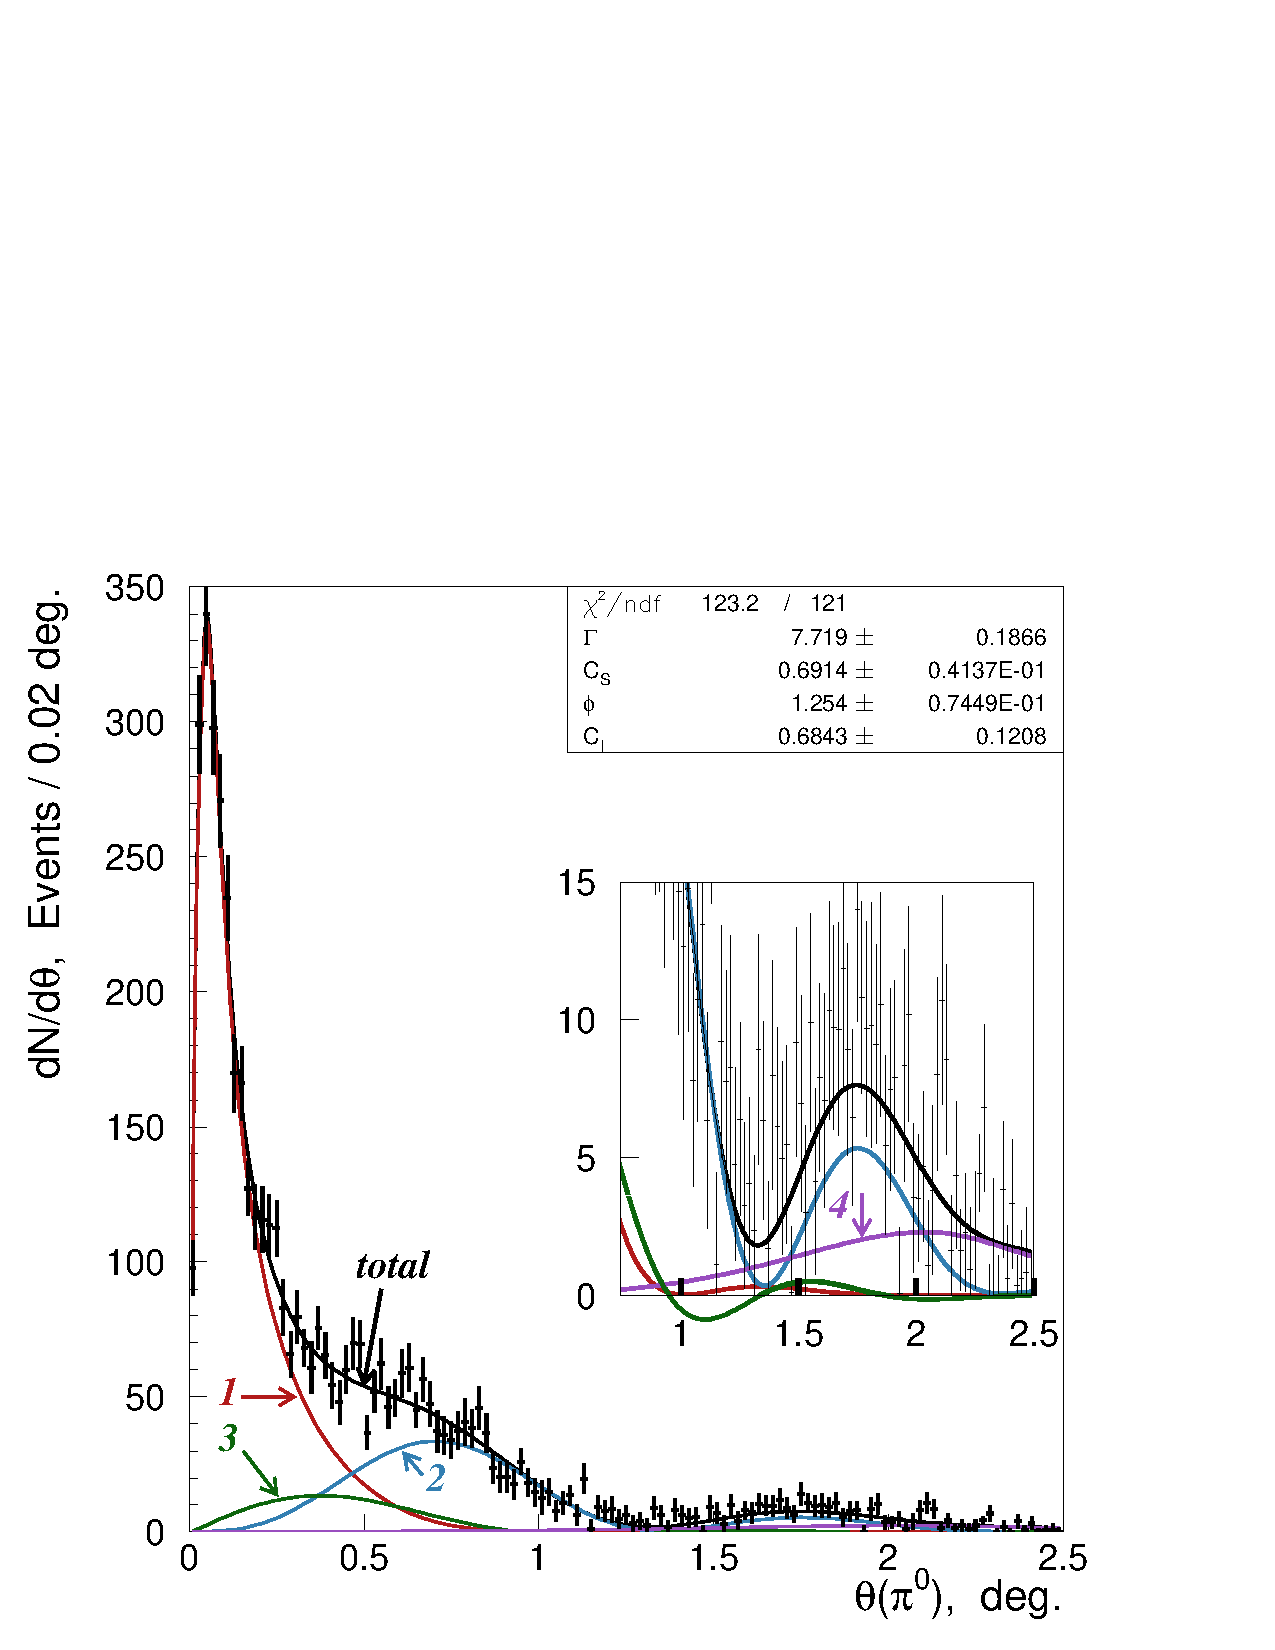
\includegraphics[width=8cm,angle=0,trim={1.5cm 0.5cm 3.5cm 9.5cm},clip]{figures/dndt_pb_partial.pdf}
\end{center}
\caption{Exclusive $\pi^0$ production yield at forward angle on lead target
  observed in the PrimEx experiment \cite{Larin:2010kq}. Curves show the various
  production mechanisms:
1 -- Primakoff, 2 -- strong coherent, 3 -- interference of first two mechanisms, 4 -- strong incoherent}
\label{fig:leaddndt}
\end{figure}




% \begin{landscape}
\begin{table}[t]
\caption{Comparison of backgrounds for the single $\pi^0$ channel and the present study for 
determination of the signal in the $\pi^0\pi^0$ channel. The relative backgrounds for this experiment
are expected to be smaller than those for the single $\pi^0$ channel.
\label{tab:Primex_sigmas}
}
\begin{center}
\begin{tabular}{|l|c|c|}
\hline
\hline 
 Integrated Fraction & $\gamma\,Pb\to \pi^0\, Pb$  & $\gamma\,Pb\to \pi^0\pi^0\, Pb$ \\  
  ($\theta <$ 1.5 degrees)                    &       & (This study) \\  \hline
  Primakoff signal  &   1.0   & 1.0   \\ \hline 
  Nuclear Coherent (NC)  & 0.39  &   0.35   \\ \hline 
  Interference  & 0.12  &  0.17   \\ \hline 
  $\gamma p \rightarrow \eta p$, BR($\eta \rightarrow 3\pi^0$)  &   -- & 0.37   \\ \hline 
  Incoherent (IC)  &   0.02  & 0.06  \\
  \hline   
  \hline
\end{tabular}
\end{center}
\end{table}





\begin{figure}[tbp]
\begin{center}
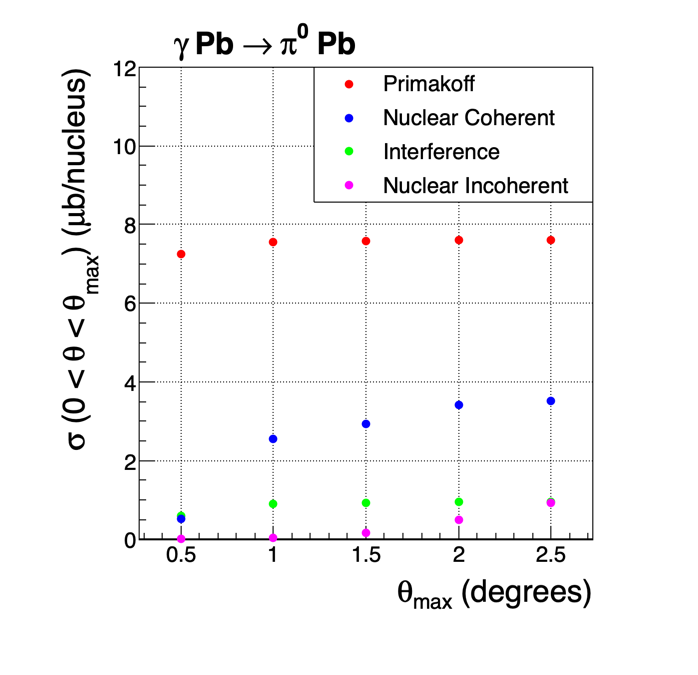
\includegraphics[width=7cm,angle=0]{figures/Primex_sigmas_c1.png}
\end{center}
\caption{Integrated angular distribution for different contributions to $\pi^0$ production in $\gamma\,Pb\rightarrow\pi^0\,Pb$ as a function of the upper limit of integration.}
\label{fig:Primex_sigmas_c1}
\end{figure}


We first classify the various backgrounds and then describe each one in
more detail. There are two-pion production data on
nuclei below 2~GeV \cite{schadm2005double} in a kinematic regime that
is dominated by nucleon resonances. However, at our energy of 6 GeV,
the exclusive production of two pions at threshold is very poorly
known experimentally, and therefore there are large uncertainties in
both the magnitude and the expected distributions of the backgrounds.
The major background comes from the $f_0(500)$ $0^{+}$ meson (also
referred to as $\sigma$-meson in the literature) that decays to two
pions. The production mechanism is expected to be very similar to
single $\pi^0$ $0^{-}$ production, since the final states are similar
except for parity. Therefore, we assume the {\em relative} background
contributions in the single $\pi^0$ reaction will be similar in our
experiment. The single-pion production distribution on a lead target
measured by PrimEx \cite{Larin:2018} is shown in
Fig~\ref{fig:leaddndt}. The relative contributions for $\pi^0$
production are plotted in Fig.~\ref{fig:Primex_sigmas_c1} as a
function of angle, highlighting the fact that the Primakoff process is
very forward peaked. The integrated fractions are also tabulated for
$\theta < 1.5$ degrees in Table~\ref{tab:Primex_sigmas} and compared
to fractions used in this study.  Production inside the nucleus will
tend to reduce hadronic backgrounds in the 2$\pi$ case due to
absorption, but we take a conservative approach and assume that absorption does
not change the general picture substantially.

 \begin{figure}[tbh]
\begin{center}
%\includegraphics[height=5cm,viewport=250 180 0 360,clip=true]{CPP_production3}
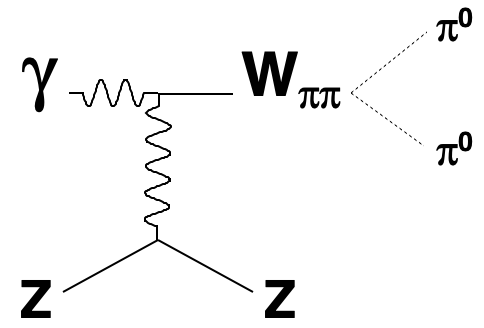
\includegraphics[height=3cm,clip=true]{figures/Diagram_Primakoff.png} \hspace{1cm}
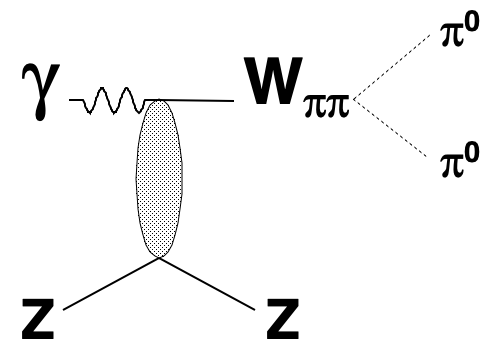
\includegraphics[height=3cm,clip=true]{figures/Diagram_hadronic.png}
\caption{Sketch of coherent two-pion production. Left) Signal: Primakoff mechanism, Right) Backgrounds: Other production mechanisms.
\label{fig:Diagram}}
\end{center}
\end{figure}

We have the following categories of backgrounds:
\begin{itemize}
\item Nuclear coherent production: In this case, the target remains
  intact. Generically, one may classify the two-pion production
  according to the sketches in Fig.~\ref{fig:Diagram}. The left-hand
  diagram represents the exchange of a virtual photon with the
  nucleus, i.e., the Primakoff mechanism. This mechanism is very long
  range, approximately 100 fm, and is affected minimally by the
  effects of shadowing or absorption.  This is the signal for the
  experiment and our goal is to determine its cross section.  The
  right-hand diagram represents the exchange of a strongly interacting
  particle (or propagator) and effectively results in the production
  of pions at the surface of the nucleus. We note that for the
  $\pi^0\pi^0$ production, pion exchange is not allowed due to charge
  conjugation conservation, while in the $\pi^+\pi^-$ case, single
  pion exchange is related to the axial anomaly ($\gamma \pi^0
  \rightarrow \pi^+ \pi^-$).  When the interaction leaves the nuclear
  target intact, the reaction is referred to as ``nuclear coherent''
  and this is one of our most serious backgrounds.
\item Incoherent production: When the interaction produces two pions
  in the quasi-elastic scattering off a single nucleon, the scattered
  target usually fragments into particles that range out in the target
  and are unobserved experimentally. This reaction occurs at larger
  $-t$ and is in general kinematically distinct from the signal. The
  angular distribution of the $\pi^0\pi^0$ momentum relative to the
  photon polarization plane is different for Primakoff and incoherent
  production.
\item Any reaction that may be confused with the signal within the
  experimental resolution or limited acceptance: An example of this
  type of reaction is Primakoff production of $\eta$ mesons, where the
  $\eta\rightarrow \pi^0 \pi^0 \pi^0$ is mis-reconstructed as a
  two-pion final state.
\end{itemize}

We note that two important backgrounds for the charged-pion
polarizability experiment do not contribute in this experiment: First,
coherent $\rho^0$ photo-production is absent in this experiment
because the $\rho^0$ decay into the $\pi^0\pi^0$ channel is prohibited
by Bose statistics.  Second, $\mu^+\mu^-$ production is also not a
background for an all-neutral final state.

\subsection{Nuclear coherent background \label{sec:NCback}}
   
The largest coherent backgrounds are  
from the photoproduction of the $f_0(500)(J^{PC}=0^{++})$ and the $f_0(980)$.
The width of the
$f_0(980)$ is fairly narrow and does not contribute directly to the strength
near threshold.
The $f_0(500)$ width is much
broader, from threshold to 800 MeV, with significant overlap in the
invariant mass region of interest.  Since the $f_0(500)$ is a scalar
particle with the same spin-parity as the $\gamma \gamma \rightarrow
\pi^0\pi^0$ final state near threshold, the azimuthal distribution of the
$\pi^0\pi^0$ momentum relative to the
photon polarization plane does not differentiate between coherent
$f_0(500)$ production and the Primakoff reaction.  
This is similar to the PrimEx-$\pi^0$ experiment, where the dominant background
was
nuclear coherent $\pi^0$ photo-production.  The approach used in the
PrimEx analysis was to measure the $\pi^0$ angular distribution,
effectively the $t$-distribution, then use theoretical calculations of
the angular distributions to separate out contributions from Primakoff
and nuclear coherent. The analysis of the $\pi^0\pi^0$ (NPP) reaction
will follow closely what was done for the PrimEx-$\pi^0$
analysis.  

We parameterize the $f_{0}(500)$ meson as detailed in
Appendix\,\ref{sec:NCsigma} and assume that the production amplitude
can be factorized as
\begin{eqnarray}
\mathcal{A} & = & \mathcal{A}_t(t) \, \mathcal{A}_W(m_{\pi\pi}) \, \mathcal{A}_\tau(\Phi, \phi, \theta),
\end{eqnarray}

where the last factor represents the angular distribution that results
in a dependence on the di-pion azimuthal angle, $\phi_{\pi\pi}$, of
the form $\mathcal{A}_\tau \propto (1 + \mathcal{P}
\cos{2\phi_{\pi\pi}}$).  The mass dependence is given by the S-wave
phase shifts that dominate the mass region below 0.8 GeV. We use the
approximate description given in
Appendix\,\ref{sec:ParmSwave}.\footnote{More detailed studies may
  require including contributions from the D-wave and S-wave, I=2,
  amplitudes.}

\begin{figure}[tbh]
\begin{center}
%\includegraphics[height=5cm,viewport=250 180 0 360,clip=true]{CPP_production3}
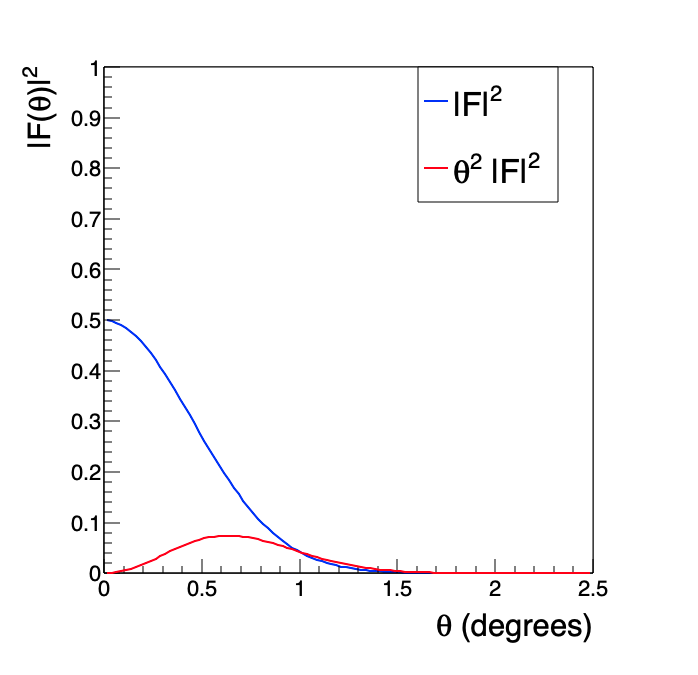
\includegraphics[height=5cm,clip=true]{figures/fit_Primakoff_sigma_c1.png}
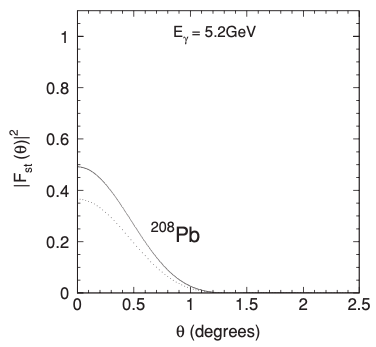
\includegraphics[height=5cm,clip=true]{figures/PRC80_2009_Fig6.png}
\caption{ Left) Approximation to strong form factor for lead, Right) Figure 6 from Ref.~\cite{Gevorkyan:2009ge} showing the calculated strong form factor for single $\pi^0$ production off a lead target.
\label{fig:strongFF}}
\end{center}
\end{figure}

We assume the $-t$ dependence of the $f_0(500)$ has a
functional form similar to single $\pi^0$ production, namely $\mathcal{A}_t(t)
\propto \sin{\theta_{\pi\pi}} \times F_{st}(t)$.  The
$\sin{\theta_{\pi\pi}}$ comes from the spin-flip required at forward
angles to produce a $0^+$ system off a spin-zero target. The factor
$F_{st}(t)$ is the strong form factor for the target, which is
approximated to match calculations for the single $\pi^0$ production
(Fig.~6 from Ref.\cite{Gevorkyan:2009ge}). Our Gaussian approximation
to the form factor is shown in Fig.~\ref{fig:strongFF} along side the
calculation for single $\pi^0$ production. Efforts are underway to
calculate the strong form factor for this
reaction.\footnote{S. Gevorkyan, private communication.}  The PrimEx
data showed that the nuclear coherent process is highly suppressed for
heavy nuclei, as shown in Fig.\ref{fig:leaddndt}.  The reason for this
suppression is $\pi^0$ absorption in the nuclear interior, making the
coherent production primarily a surface effect.  For NPP it is
expected that suppression of the nuclear coherent process will be
approximately twice stronger than that seen in PrimEx because two
pions are produced in NPP as compared to a single $\pi^0$ in PrimEx.

 \begin{figure}[tbp]
\begin{center}
%\includegraphics[height=5cm,viewport=250 180 0 360,clip=true]{CPP_production3}
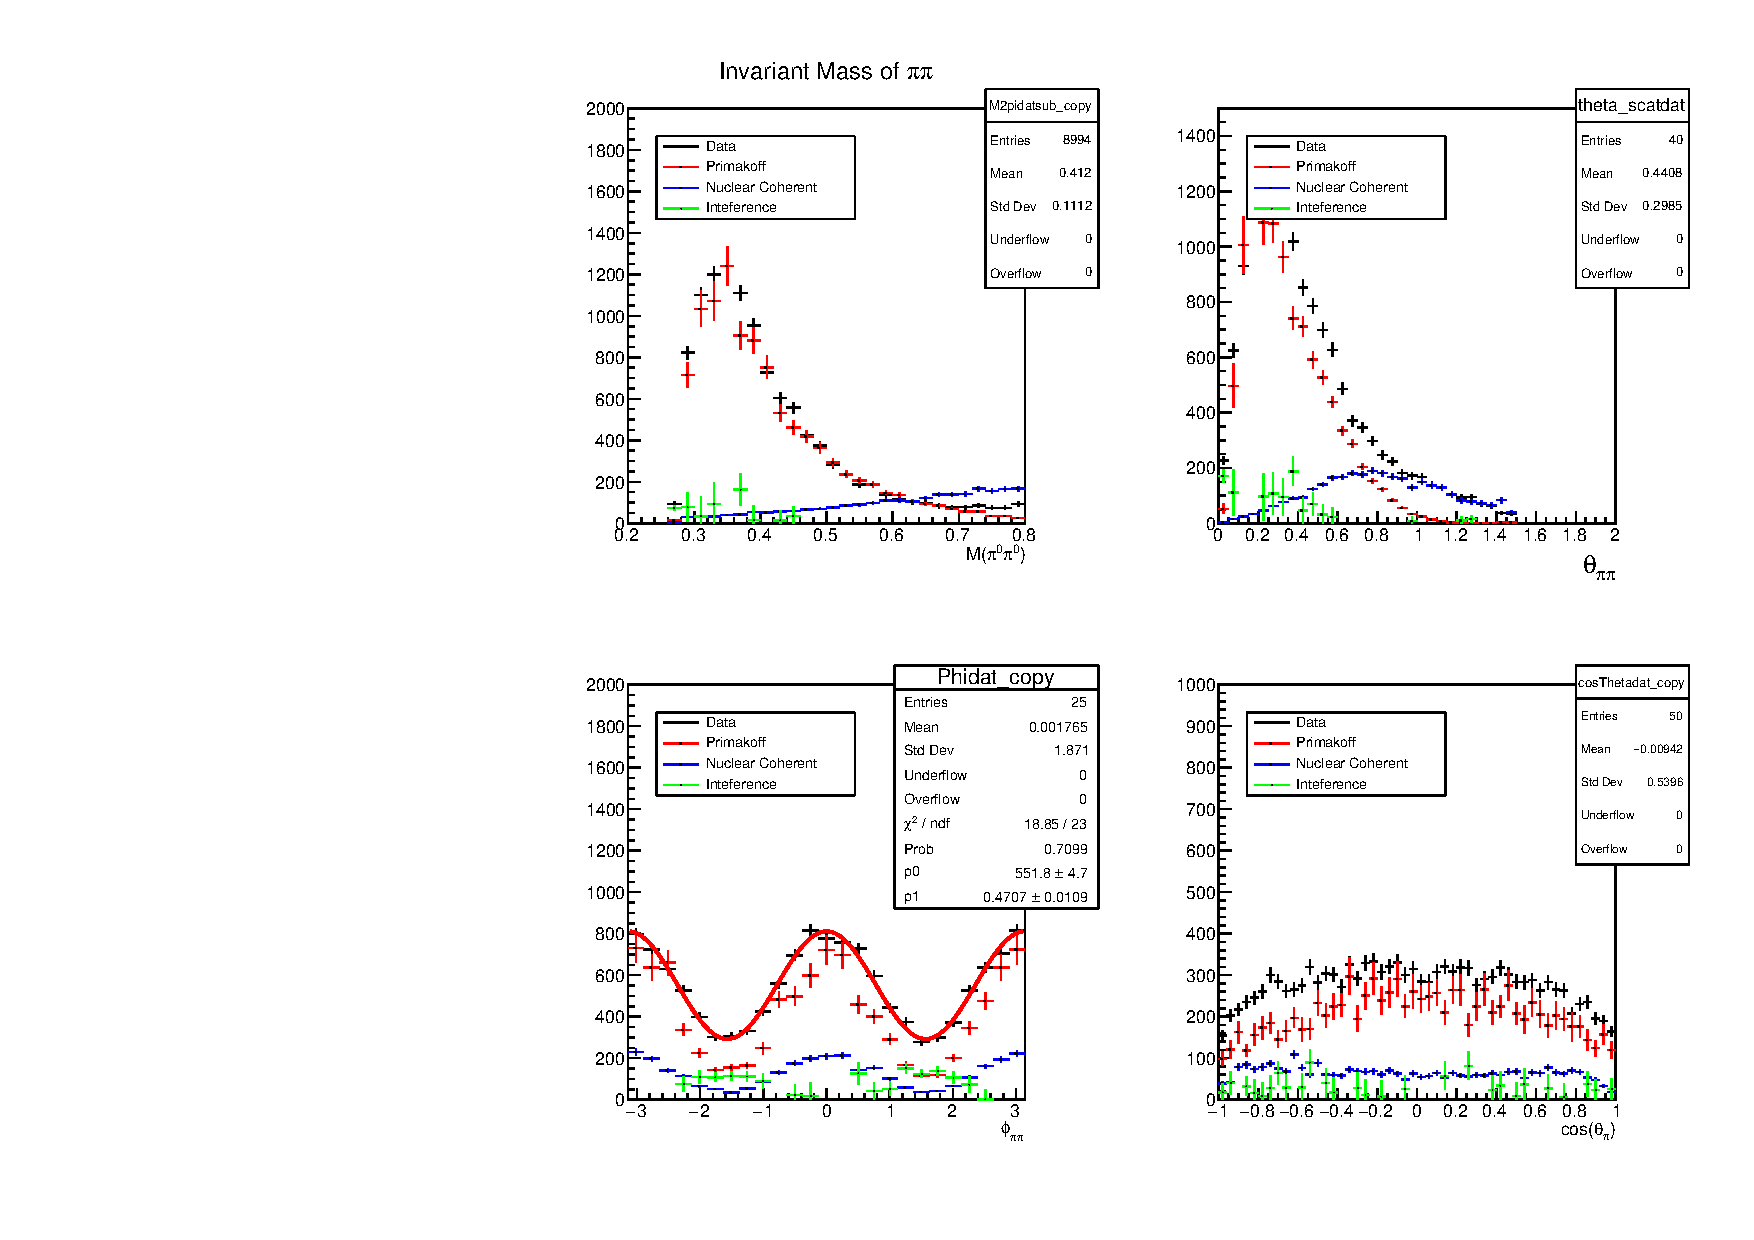
\includegraphics[height=15cm,clip=true]{figures/twopi_primakoff_DSelect_test_File_100000_decomposition_PrimNC.pdf}
\caption{Kinematic distributions for the Primakoff signal and nuclear coherent background only are shown for reference. The MC data (black) are fitted to the sum of the signal and NC background including the interference between amplitudes. 
Top left) 2$\pi$ mass, Top right) 2$\pi$ scattering angle, Bottom left) 2$\pi$ azimuthal angle, 
Bottom right) Polar angle of one pion in the $2\pi$ center-of-mass.
\label{fig:decomposition_PrimNC}}
\end{center} 
\end{figure}

Fig.~\ref{fig:decomposition_PrimNC} shows distributions of interest
for a sample of $\pi^0\pi^0$ Primakoff and nuclear coherent background
events simulated in approximate proportion to that observed in single pion
production. The strong phase between the two production mechanisms is
set to 75 degrees for this simulation, where an angle of zero produces
maximum interference. This angle must be determined experimentally.
The 2$\pi$ mass and the 2$\pi$ scattering angle distributions are
shown in the top two panels. The Primakoff signal peaks at the
2$\pi$-mass threshold and at about 0.2 degrees, whereas the nuclear
coherent signal rises linearly from 2$\pi$ threshold, as expected for
$f_0(500)$ production, and peaks at an angle of about 0.8
degrees. The azimuthal angular distribution is the same for both
signal and background and has no discriminating power. The angular
distributions of the pions in the center of mass of the $2\pi$ system
are all uniform, and as such do not help in distinguishing the signal
from the nuclear coherent background.

\begin{figure}[tbp]
\begin{center}
%\includegraphics[height=5cm,viewport=250 180 0 360,clip=true]{CPP_production3}
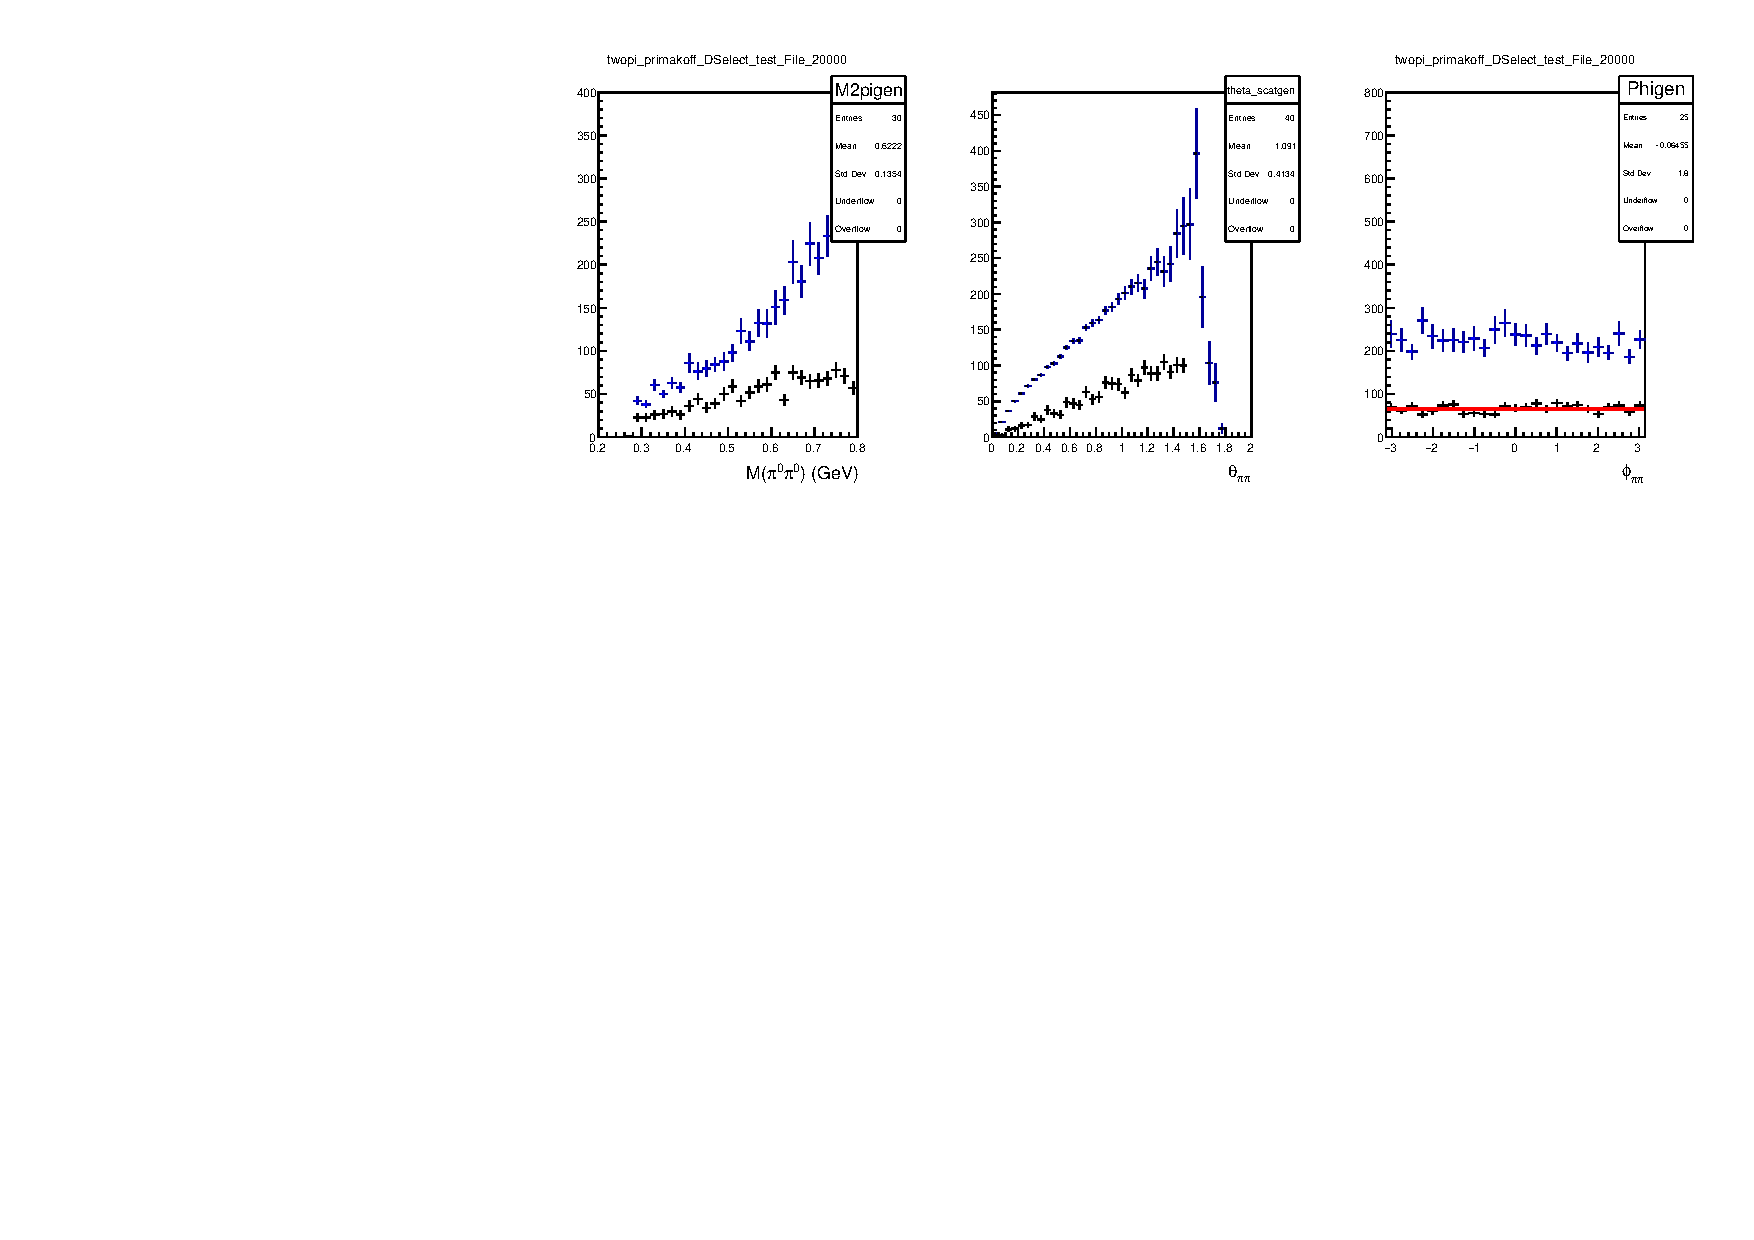
\includegraphics[width=16cm,clip=true]{figures/twopi_primakoff_DSelect_test_File_20000_IC.pdf}
\caption{Distributions for the incoherent production off free nucleons. The blue crosses represent the generated distributions and the black crosses represent the kinematically fit accepted distributions.
Left) 2$\pi$ mass. Center) 2$\pi$ scattering angle. The drop of the generated distribution at 1.5 degrees is due to an analysis cut. Right) 2$\pi$ azimuthal angle.
\label{fig:IC}}
\end{center} 
\end{figure}

\subsection{Incoherent two-pion production}
In addition to the coherent production of two pions off the nucleus,
two pions may also be produced via the elementary reaction $\gamma
N\to \pi^0 \pi^0 N$, breaking up the nucleus in the process. We model
the incoherent background with a mass distribution given by the
$f_0(500)$, but with an exponential $t$ dependence given by $e^{Bt}$,
with $B=3.6$ GeV$^{-2}$. The slope is taken from
Ref.\cite{Battaglieri:2009aa} and has very large
uncertainties. However, as long as the slope is small compared to
Primakoff production, which has an effective slope of $B\sim560$
GeV$^{-2}$, it does not change the picture. The mass and angular
dependencies are shown in Fig.~\ref{fig:IC}. The strength is small at
threshold and at small angles, where Primakoff is strongest. The
azimuthal angle is flat, so the photon polarization can also
discriminate against this background.

The cross section for this reaction on free protons is relatively
large, about 140 nb/nucleon for $0.3 < M_{\pi\pi} < 0.8$
GeV.\footnote{The cross section is estimated from the S-wave
  production of the $f_0(500)$ meson extrapolated to small $-t$ from
  data archived in the {\em hepdata.net} database and reported in
  Ref.~\cite{Battaglieri:2009aa}. See Appendix\,\ref{sec:NCsigma} for
  more information. A factor of one half is applied to the measured
  cross section for $\pi^+\pi^-$.} However, this process is strongly
suppressed in nuclei by Pauli blocking and by pion absorption. The
Pauli suppression is proportional to $1-G(t)$, where $G(t)$ is a
nuclear form factor and has the limit of $G(t)\to1$ as $-t\to0$
\cite{Gevorkyan:2009ge,primex_inc}. In the case of single $\pi^0$
production, incoherent scattering contributes at the level of a couple
of percent, and we expect it to be suppressed more strongly in $2\pi$
production. See Appendix\,\ref{sec:SigmaScaling} for
details. Therefore, we expect this background to be about three times
smaller than what is used in the present studies.

\begin{figure}[tbp]
\begin{center}
%\includegraphics[height=5cm,viewport=250 180 0 360,clip=true]{CPP_production3}
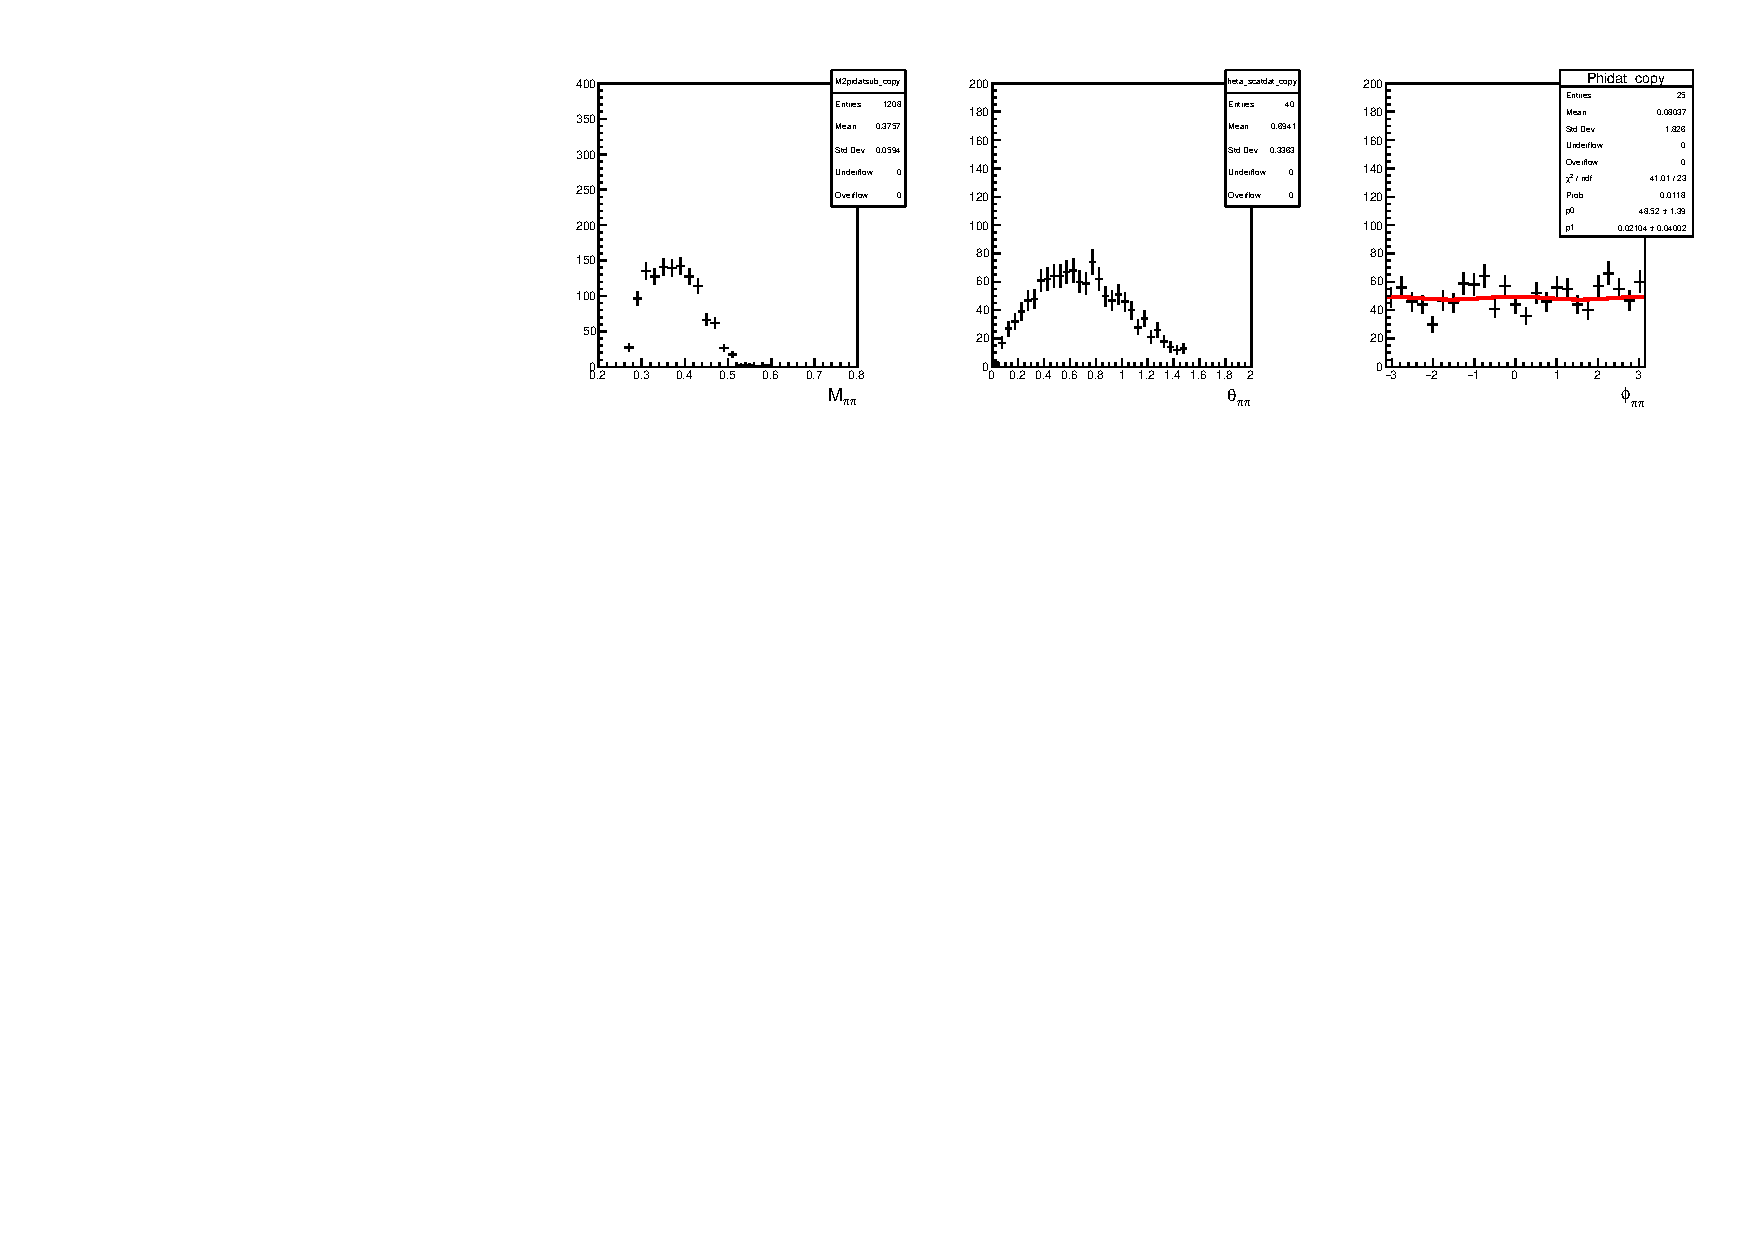
\includegraphics[width=16cm,clip=true]{figures/BrokenEtasPrim.pdf}
\caption{Kinematically fit distributions for $\eta$'s that decay to 3$\pi^0$, but get reconstructed as a 2$\pi^0$ final state (broken $\eta$'s).
We generated the sample using the {\em gen\_EtaPb} event generator which simulates the Primakoff mechanism. The distributions produced from the NC mechanism are similar. 
Left) 2$\pi$ mass. Center) 2$\pi$ scattering angle. Right) 2$\pi$ azimuthal angle.
\label{fig:eta}}
\end{center} 
\end{figure}



\subsection{Mis-identified backgrounds}

There may be important backgrounds that are mistaken for the signal
due to mis-identification. These may include

\begin{enumerate}[label=(\roman*)]
    \item coherent production of $\eta$ followed by $\eta\rightarrow
      \pi^0\pi^0\pi^0 \rightarrow
      \gamma\gamma\gamma\gamma(\gamma\gamma)$, where only four photons
      are reconstructed.
    \item production of nucleon resonances that contribute to the
      $\gamma N \rightarrow N \pi^0\pi^0$ final state. This
      contribution is expected to be small based on the experience of
      other Primakoff experiments.
\end{enumerate}
The most important background from mis-identification is due to
$\eta$ production, where the $\eta$ decays to three $\pi^0$s but is
reconstructed with a reasonable kinematic fit probability as a 2$\pi^0$ final
state. We refer to these as ``broken" $\eta$'s. As with $\pi^0$
production, $\eta$ mesons may be produced via the Primakoff process,
by the NC process or by quasi-elastic scattering from individual
nucleons. The first two mechanisms are the most pernicious, as the
incoherent production produces events that fall outside the typical
signal kinematics.  The incoherent production was investigated using
the {\em genEtaRegge} event generator \cite{hdnote2437}. As expected,
the resulting distributions are very similar to those from incoherent
2$\pi$ production described in the previous section.  If $\eta$'s are
produced via the Primakoff and/or NC mechanisms, they may reconstruct
as a 2$\pi$ final state if one of the decay pions is low energy and
goes undetected. The probability for this to happen is at the percent
level.  We describe these production mechanisms in more detail next.

Two samples of $\eta$ events were generated, one corresponding to
Primakoff-$\eta$ production and the other due to NC production of
$\eta$'s. These are two-body reactions, so they only differ in the
angular distribution of the produced $\eta$, or equivalently their
$t$-distribution. In principle these mechanisms interfere, but we
generated the samples independent of one another and assumed a
uniform azimuthal angular distribution. The events were then processed
through the Geant4 Monte Carlo, which decayed them according to their
nominal branching fractions, and then {\em mcsmear}. These steps were
followed by the reaction filter that analyzed the events just as if
they were signal, i.e., treated events as $\gamma Pb \rightarrow Pb\,
\pi^0 \pi^0$ with a kinematic fit assuming the recoil target nucleus
was missing.
%Standard missing-mass and $\chi^2$ cuts were used to pick out events that faked the signal. 
%It turns out that the angular distribution of broken $\eta$'s produced from the NC process are not very different than those for the Primakoff production shown in the figure.

We used a couple of very simple but powerful selection cuts to
eliminate the $\eta$ background. The cuts include a selection on the
missing mass squared ($|MM - M_{Pb}{^2}| < 0.1$ GeV$^2$) and a cut on
the $\chi^2 < 5$ of the kinematic fit to $\gamma\,Pb\rightarrow
\pi^0\pi^0 (Pb)$ with a missing recoil. In the analysis we also
restrict the $2\pi$ scattering angle ($\theta_{\pi\pi} <1.5$ degrees),
which further constrains the range of missing mass. The result of
these selections, which have been applied uniformly to signal and
background, reduce the contamination from this source to about 37\% of
the signal. The distributions of the accepted events for the
Primakoff-$\eta$ mechanism are shown in Fig.\ref{fig:eta}.  These
selections are illustrative and will allow us to achieve our
experimental goals but further optimizations may have to be done. We note that
the relative number of mis-identified $\eta$'s in the experiment will
be determined empirically from the measured rate of fully
reconstructed $\eta\rightarrow\pi^0\pi^0\pi^0$ events.

The number of generated Primakoff-$\eta$ events was determined by
using the scaling rules described in
Appendix\,\ref{sec:SigmaScaling}. The rate of Primakoff-$\eta$
production was determined relative to Primakoff-$\pi^0$ (0.28) and the
results in the appendix (Eq.\,\ref{eq:sigpipi_over_sigpi}) used to
determine this rate relative to Primakoff-$\pi^0\pi^0$ (1/0.05),
resulting in $\sigma_\eta/\sigma_{\pi^0\pi^0} \sim 6$. We assume that
the fraction of NC-$\eta$/Primakoff-$\eta \sim$ 1/3. The events from
each sample were combined in this ratio as backgrounds for use in the
study of the extraction of the signal.

 \begin{figure}[tbp]
\begin{center}
%\includegraphics[height=5cm,viewport=250 180 0 360,clip=true]{CPP_production3}
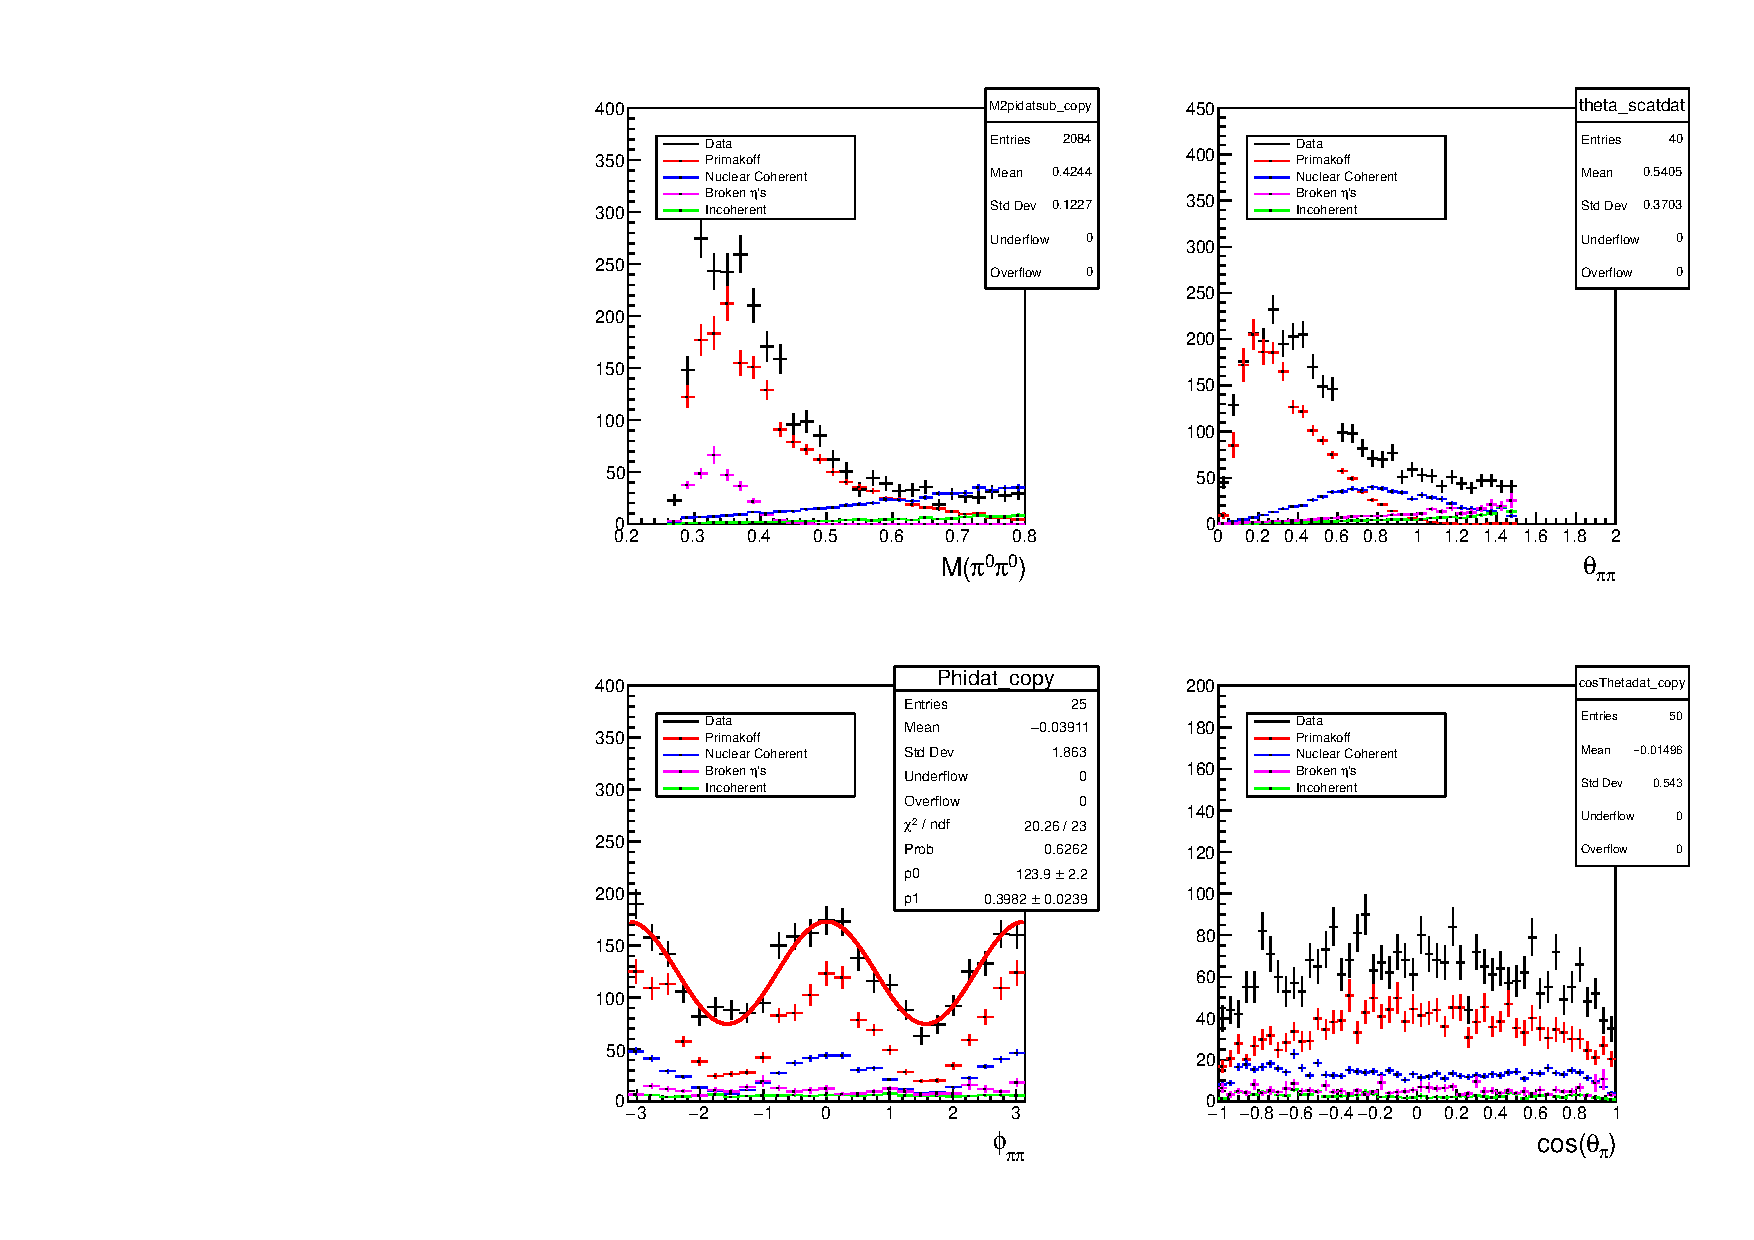
\includegraphics[height=15cm,clip=true]{figures/twopi_primakoff_DSelect_test_File_100000_decomposition_PrimNCICeta.pdf}
\caption{Results of the amplitude fit to the MC data (black points) to extract the amplitudes for the $\pi^0\pi^0$ Primakoff signal, nuclear coherent background, broken $\eta$ distributions and incoherent background.
Top left) 2$\pi$ mass, Top right) 2$\pi$ scattering angle, Bottom left) 2$\pi$ azimuthal angle, 
Bottom right) Polar angle of one pion in the $2\pi$ center-of-mass.
\label{fig:decomposition_PrimNCICeta}}
\end{center} 
\end{figure}

\section{Extraction of the Primakoff signal \label{sec:signalfit}}

The $\pi^0\pi^0$ Primakoff signal is determined using an amplitude
fit\footnote{AmpTools, https://github.com/mashephe/AmpTools/wiki.} to
all data simultaneously. It assumes that the mass and angular
distributions are known for each of the contributions to the 2$\pi$
sample. A complex scaling factor is determined for each contribution
by doing an unbinned maximum likelihood fit to the event sample. The
result of such a fit to the sample that includes the Primakoff and NC
processes only, has been shown in Fig.~\ref{fig:decomposition_PrimNC}. The
fit to the MC data that includes the Primakoff-$\pi^0\pi^0$ signal,
and backgrounds from NC-$\pi^0\pi^0$, incoherent production and broken
$\eta$'s, is shown in Fig.~\ref{fig:decomposition_PrimNCICeta}. The
generated samples correspond approximately to the expected number of
events expected for the experiment. The three kinematic quantities
that have the most discriminating power between the signal and background
are the
2$\pi$ mass $M_{\pi\pi}$, the 2$\pi$ scattering angle
$\theta_{\pi\pi}$ and the azimuthal angle $\phi_{\pi\pi}$. The fit
uses all the kinematic information contained in the event sample to
determine the fraction of signal and background components that are
present. A good fit is obtained to the data and the Primakoff signal
is determined. The statistical uncertainties as a function of
$M_{\pi\pi}$ are obtained directly from the fit (top left plot in
Fig.~\ref{fig:decomposition_PrimNCICeta}). We estimate the systematic
uncertainty (3\%) in the extraction of the signal by assuming that the
number of broken $\eta$'s can be known with an uncertainty of 25\%.


%<><><><><><><><><><><><><><><><><><><><><><><><><><><><><><><><><><><><><><><><><><><><><>
 % Analysis of existing data
 %<><><><><><><><><><><><><><><><><><><><><><><><><><><><><><><><><><><><><><><><><><><><><>

\section{Analysis of existing data}
We investigated the challenges of reconstructing 2$\pi^0$ final states
with a missing recoil proton using the 2017 GlueX data taken with a
hydrogen target and the 2019 PrimEx-Eta data with beryllium and helium targets.
This is a useful exercise to verify that nearly elastic 2$\pi^0$
events can be detected with GlueX and to check the resulting
resolutions with real data. Unfortunately, the high backgrounds with these targets prevented the extraction of a Primakoff signal.
\subsection{Hydrogen target}
  We selected and reconstructed events that matched the
topology of the reaction $\gamma p\rightarrow \gamma \gamma \gamma
\gamma\, (p)$ with a missing proton. A kinematic fit was performed
that conserved energy and momentum and imposed a vertex constraint at the center of the target cell
($z=65$~cm). The fit was required to converge. We note
that even though the vertex was
fixed at 65~cm to perform the fit, the actual target extends from 50
to 80 cm. Several other nominal selection criteria were imposed to clean up
the event sample, including the absence of charged tracks and a requirement
that there be no missing
energy. No constraints were imposed on the $\pi^0$ mass to allow study of
backgrounds. In addition accidental background subtractions were performed.
\begin{figure}[tph] 
\centering
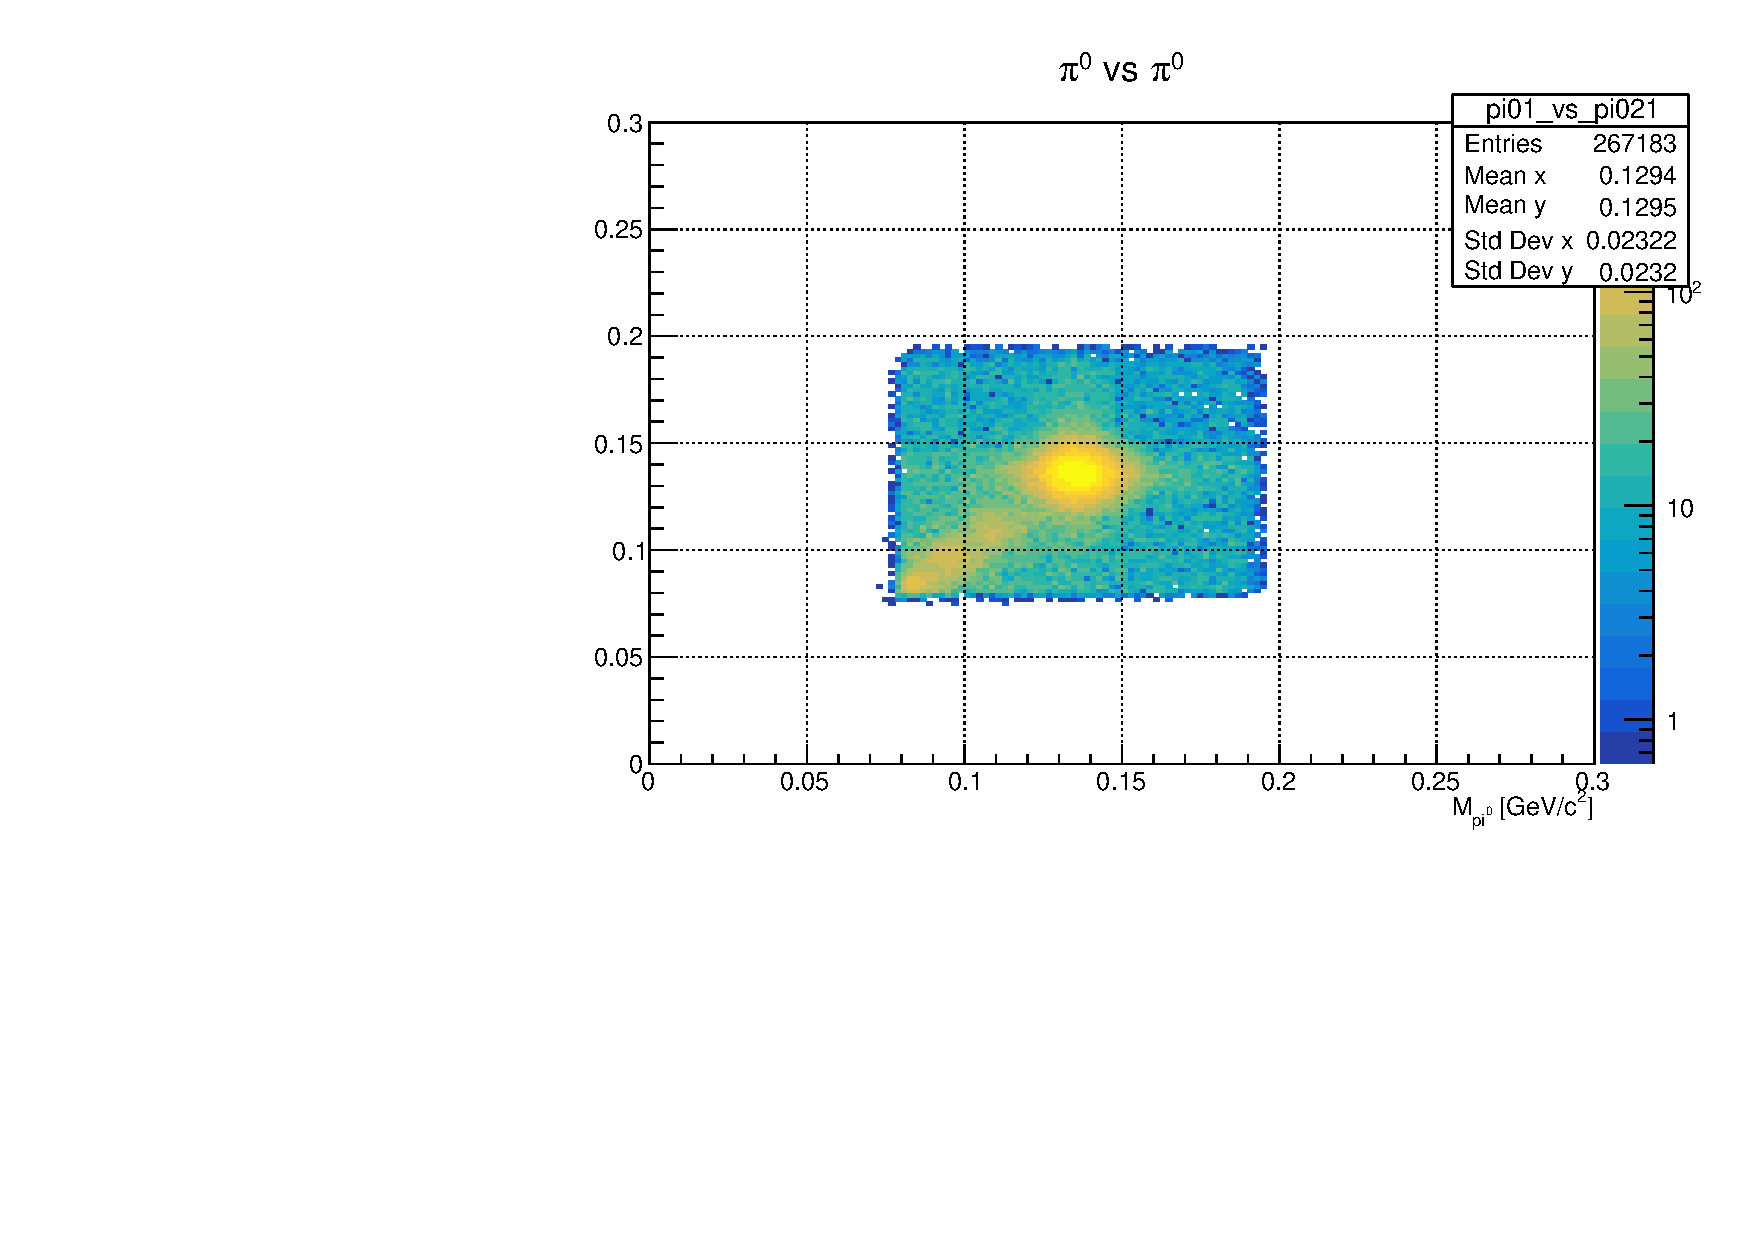
\includegraphics[width=4.75in]{figures/pi0VSpi0.pdf} \\
\centering
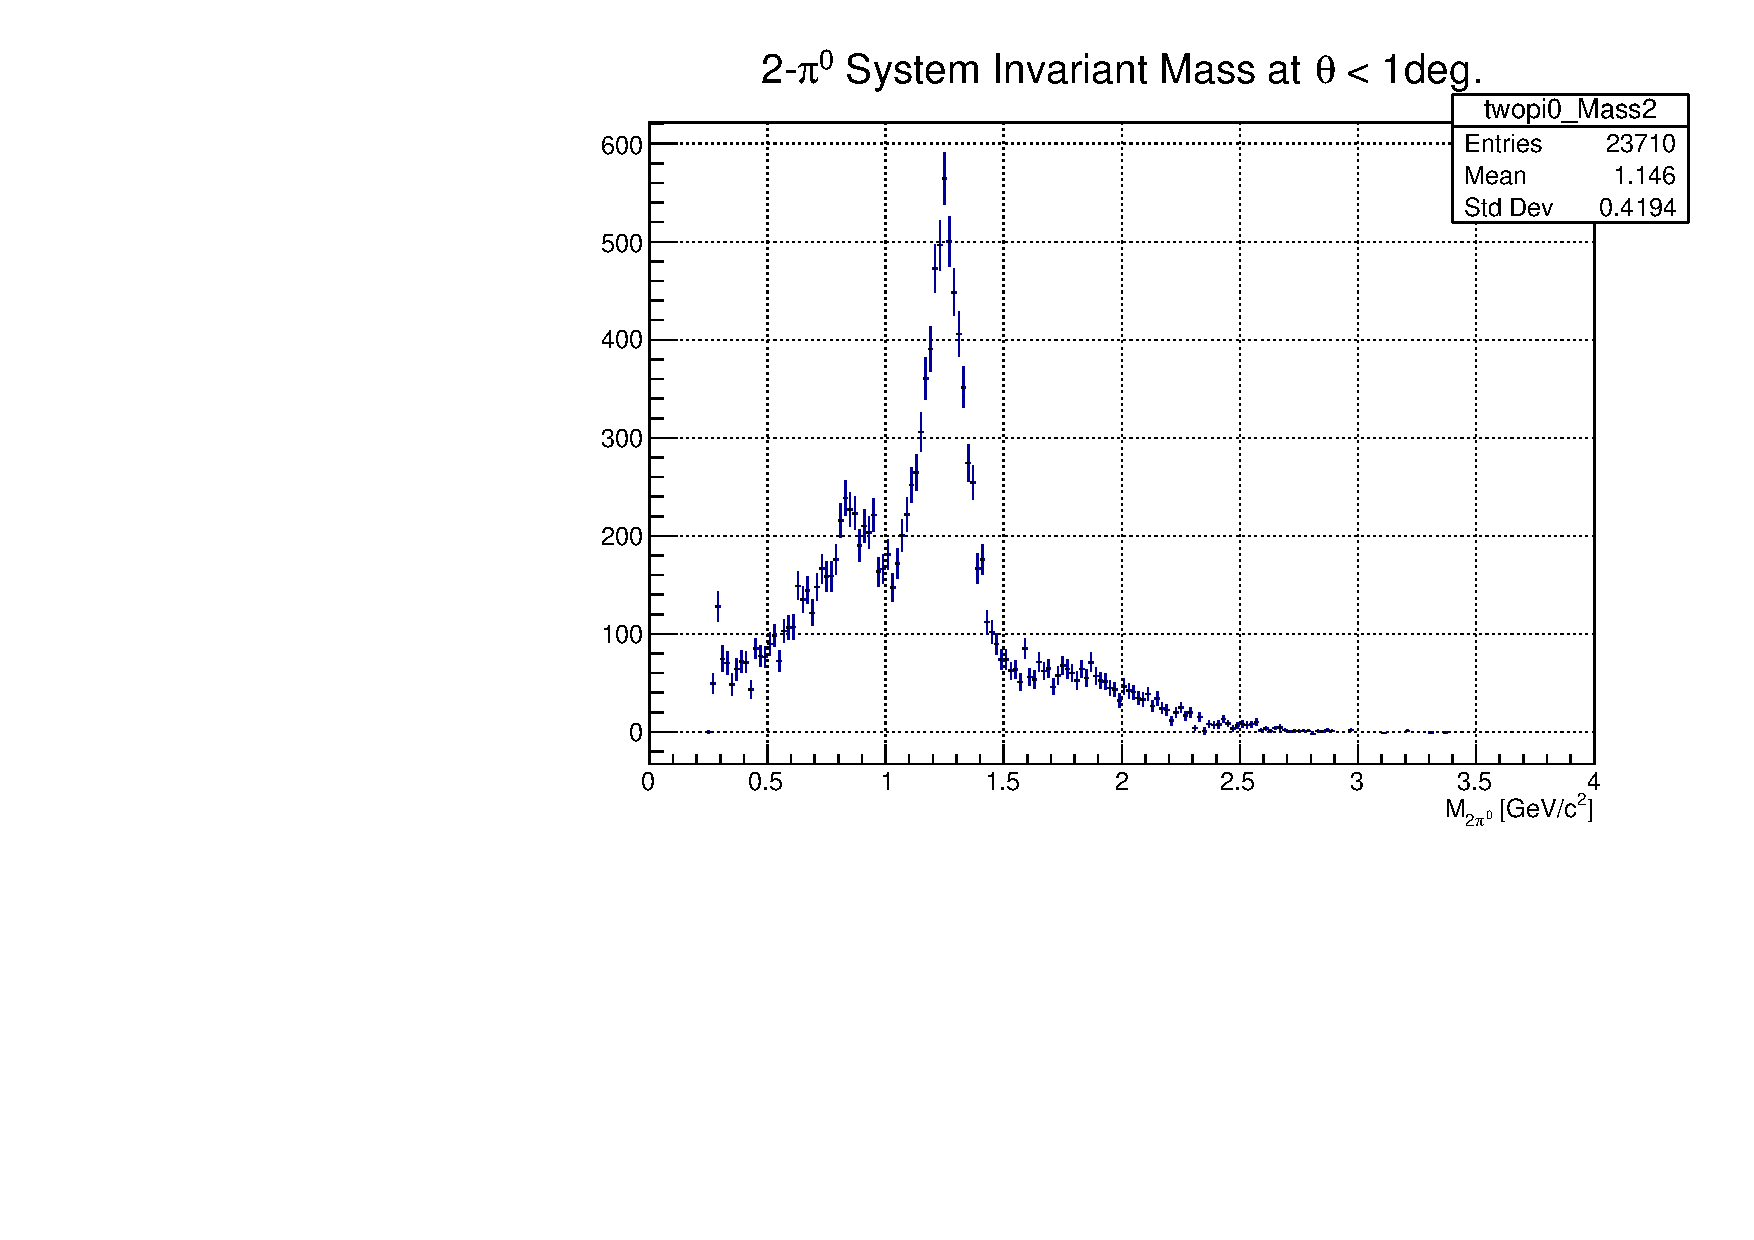
\includegraphics[width=4.75in]{figures/TwoPiInvMass.pdf}
\caption{Experimental distributions from the 2017 GlueX data set
  analyzed as $\gamma p\rightarrow \gamma \gamma \gamma \gamma\, (p)$
  with a missing proton. Top: Two photon invariant mass of one pair vs
  the two photon invariant mass of the second pair. Bottom: 2$\pi$
  mass distribution selecting events with the reconstructed photon
  pair masses close to the $\pi^0$ mass as shown above. The plot also
  requires that the angle of the two-pion system be less than 1
  degree.
\label{fig:TwoPiInvMass}}
\end{figure}

The invariant mass distribution in two dimensions, for a given photon pair versus that for
the other pair in these four-photon events shows a
strong $\pi^0$ peak, as shown in the top of
Fig.~\ref{fig:TwoPiInvMass}. There are background events that fall
under the two $\pi^0$ peaks, which require further study,
nevertheless, using the selection of photon pairs that reconstruct to
the $\pi^0$, we can plot the 2$\pi^0$ mass spectrum (bottom of
Fig.~\ref{fig:TwoPiInvMass}). The mass spectrum has recognizable
features, in particular the prominent $f_2(1270)$ that decays to
$\pi^0\pi^0$ 85\% of the time. The structure at $M_{\pi\pi}\sim$0.8~GeV
appears too low for the $f_0(980)$ and is present in a location
where the Crystal Ball data \cite{Marsiske:1990hx} shows a low
yield. The yield for $M_{\pi\pi}<$0.5 GeV is consistent within a
factor of two of the relative yield compared to the $f_2(1270)$ peak in
the Crystal Ball data. This analysis demonstrates that these neutral
events can be analyzed in our detector under circumstances significantly more
challenging than we anticipate for the Primakoff
experiment. In particular, for the Primakoff experiment, we will have
a solid nuclear target with little extent in $z$ that will allow valid geometrical constraints
and thus improving the resolution on missing momentum in the reaction. This will
make the kinematic fitting more effective.

It is evident from the top plot in Fig.~\ref{fig:TwoPiInvMass} that a cut
on the invariant mass of one reconstructed $\pi^{0}$ will reduce the
background on the other $\pi^{0}$ significantly. This is shown in
Fig.~\ref{fig:pi0yield} where a cut on the invariant of one $\pi^{0}$
significantly reduces the background in the other while keeping the
main signal mostly undisturbed.
\begin{figure}[htp]
\centering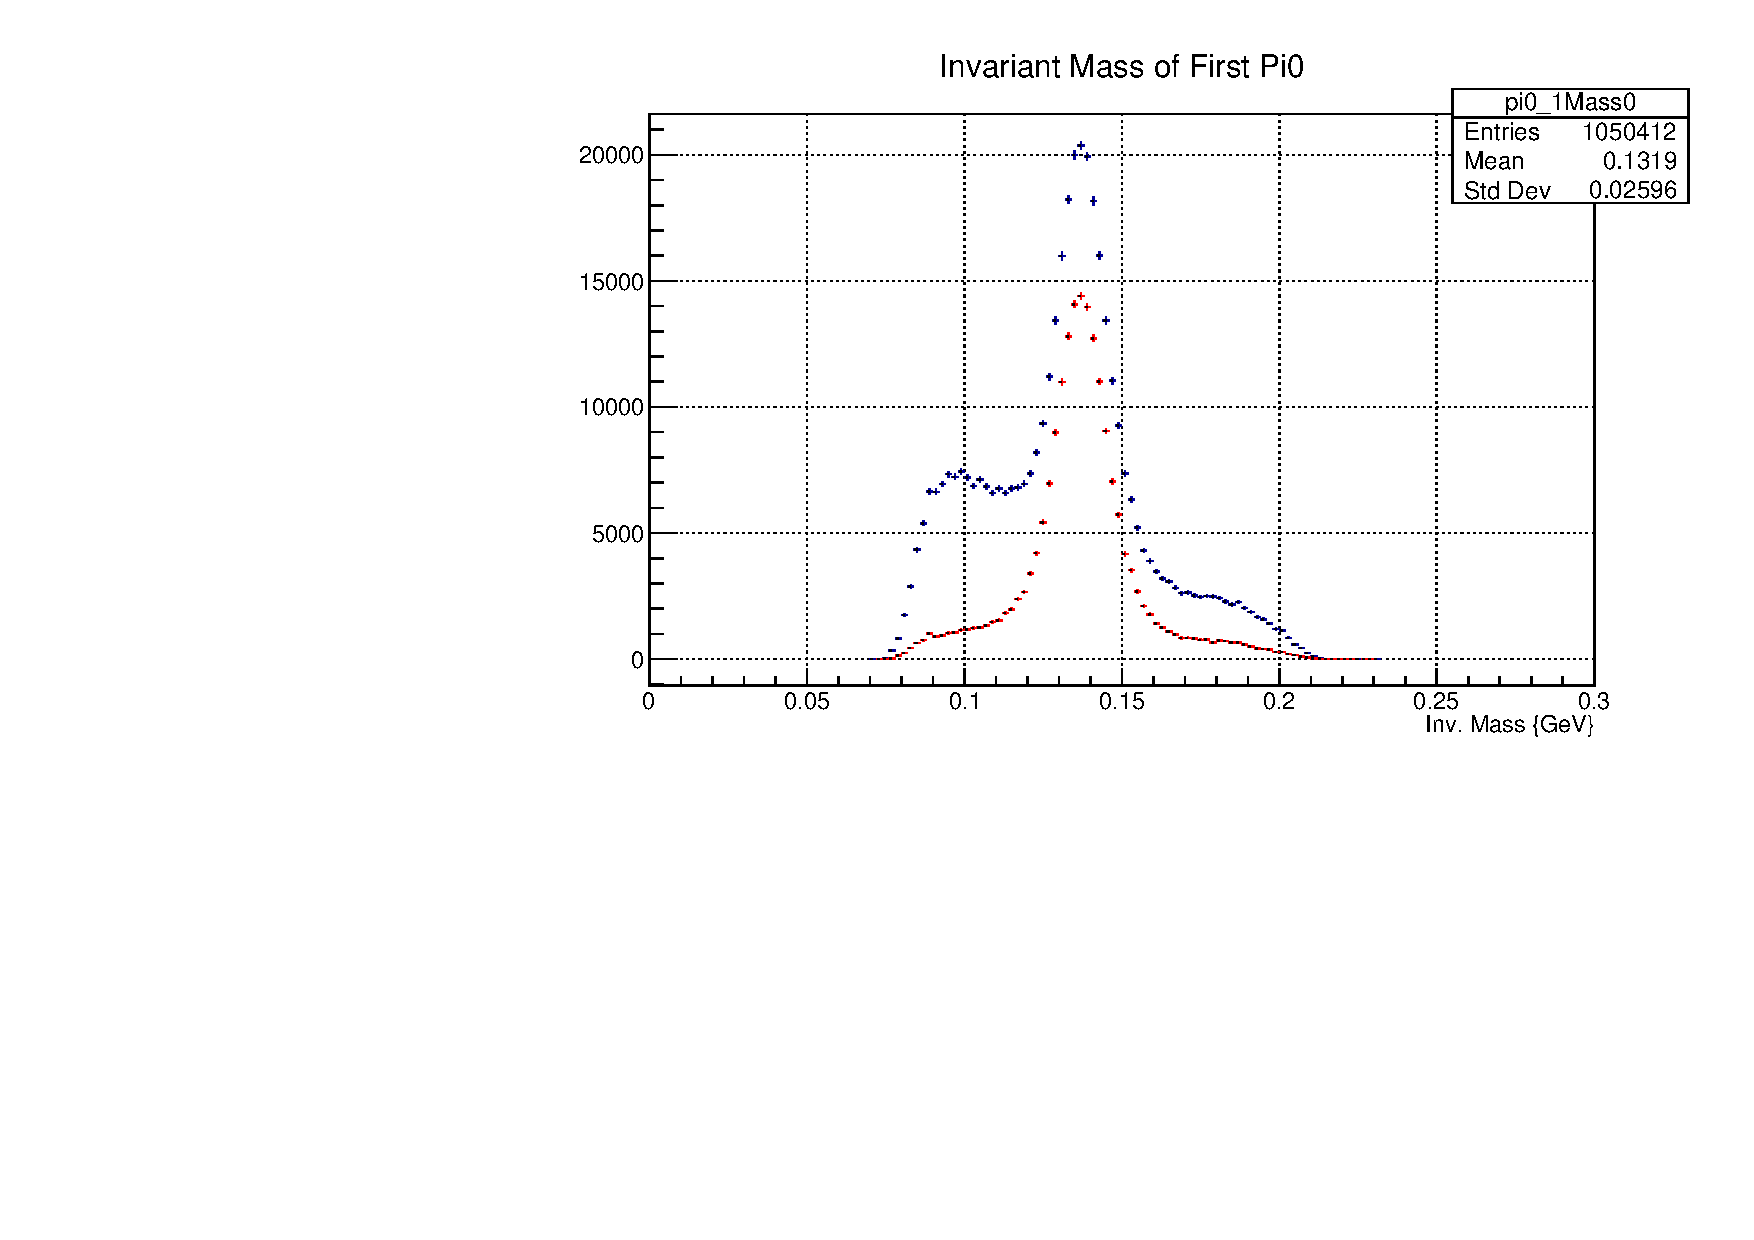
\includegraphics[width=4.75in]{figures/pi0_inv_mass_withpi02cut.pdf}
\caption{Invariant mass of the two-photon system with (red) and
  without (blue) a cut on the invariant mass of the second pair of
  photons.
\label{fig:pi0yield}}
\end{figure}

These photons are detected by the lead-glass calorimeter whose energy resolution is the
main contribution to the resolution of the reconstructed $\pi^{0}$
mass. A lead-tungstate calorimeter with a substantially better energy
resolution would yield a significant improvement in the signal-to-noise
ratio as the width of the reconstructed $\pi^{0}$ would be
smaller by about a factor of two.

\subsection{Helium and beryllium targets}

The PrimEx-Eta experiment collected valuable data on light nuclear
targets ($^4$He and $^9$Be) in 2019. Analysis of two-neutral-pion-system
photoproduction on these nuclei gives a good estimate of the
main background sources, signal-to-background levels, and the Hall-D
detector resolution for the main kinematic variables. The total PrimEx-Eta luminosity
corresponds to approximately one day on
a 5\% radiation length beryllium target and 18 days on a
4\% radiation length helium target at 200~nA electron beam
current and a $10^{-4}$ radiation length amorphous tagger
radiator. The beryllium target has a thickness of only 1.5~cm
(compared to the 30~cm liquid helium and hydrogen targets), which allows
constraining interaction point (important for reconstruction of neutral pions
without any additional vertex information from the
tracking system).  First we identified the two neutral pion
process using the ratio of energy of the two pions to the
initial beam energy with the expected recoil energy
subtracted. Fig.$\,$\ref{fig:pi0elastbe} shows this distribution for
pions detected in FCAL and time accidentals and out-of-target beam
interaction subtracted.
\begin{figure}[!h]
\centering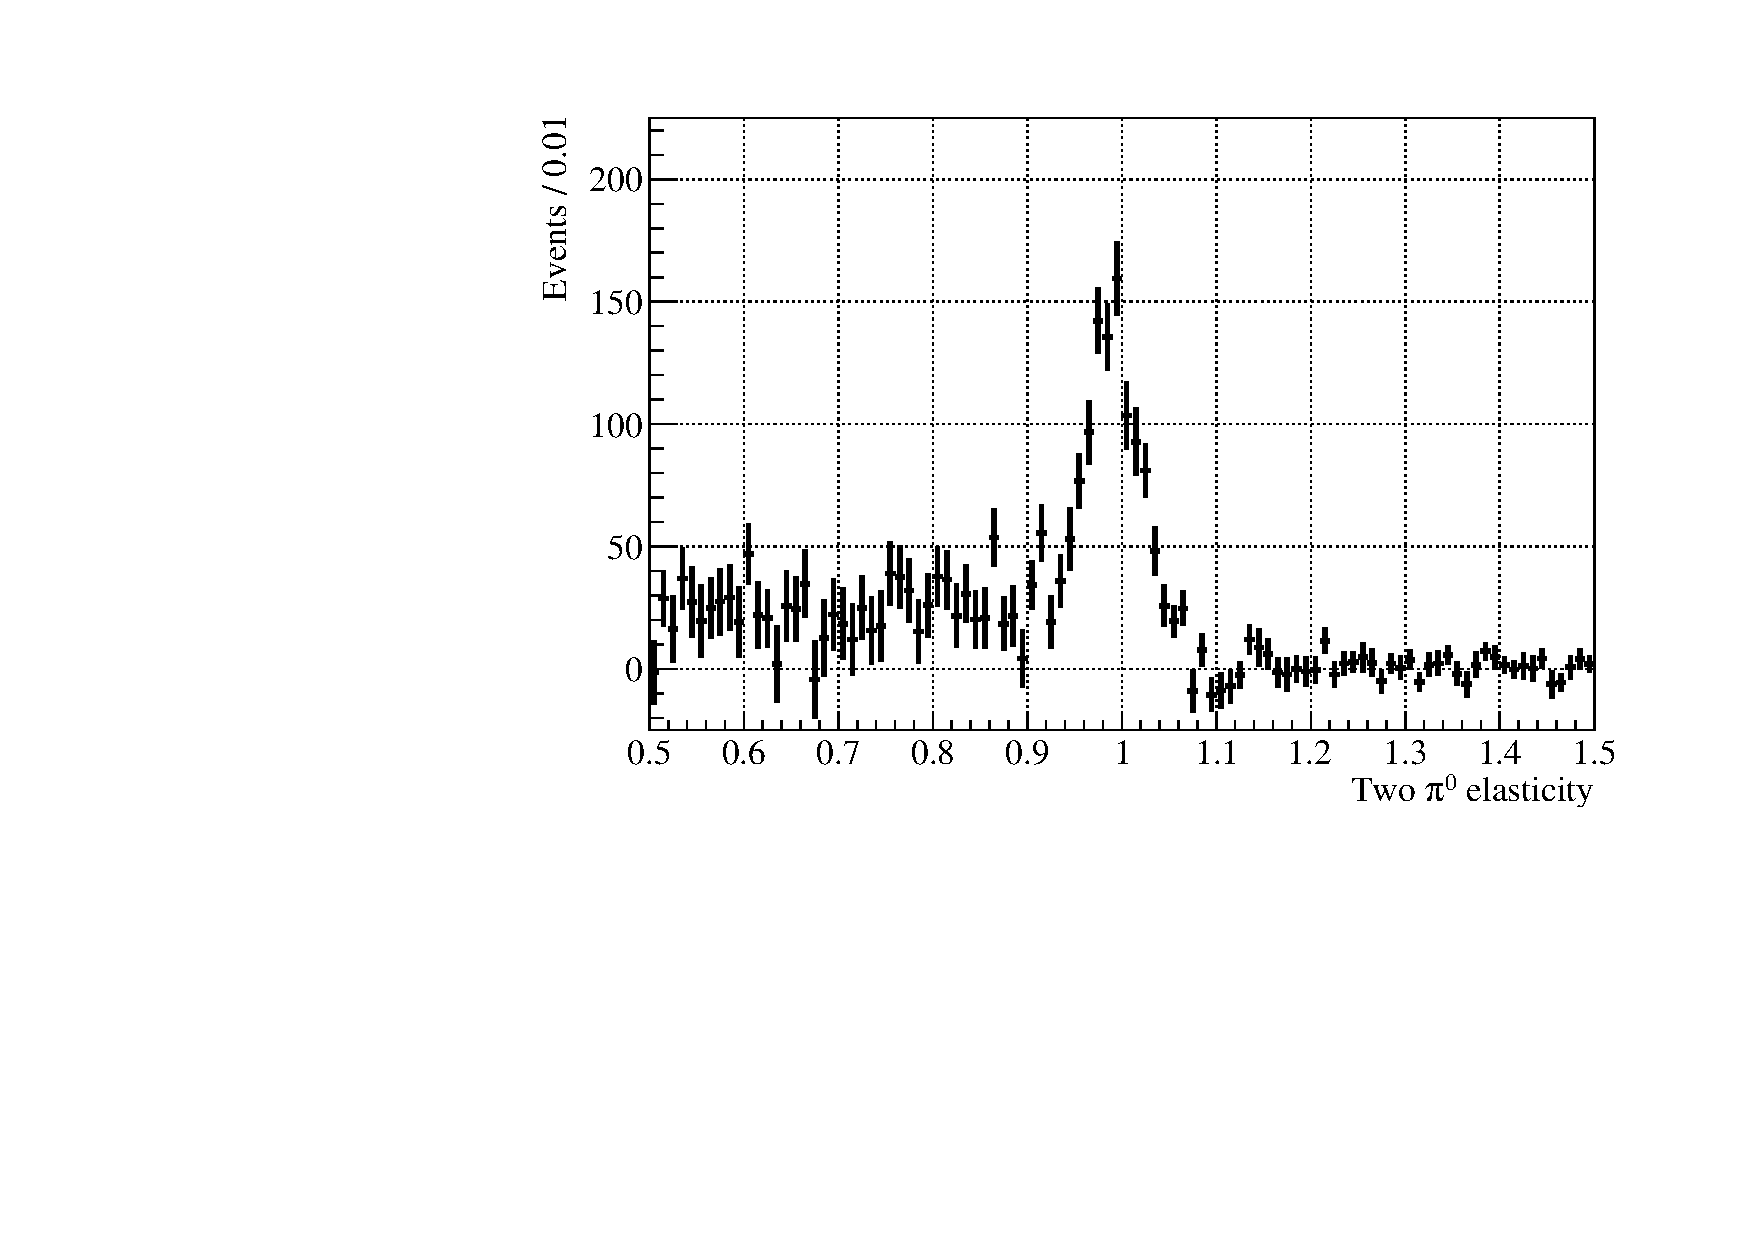
\includegraphics[width=4.75in]{figures/be_elast1.pdf}
\caption{Two neutral pion elasticity (ratio of two-pion energy to that expected for exclusive production) for the beryllium target.
\label{fig:pi0elastbe}}
\end{figure}
We first required exactly four showers to be detected in FCAL and no
extra showers in BCAL and COMCAL, a minimum shower energy of
0.5~GeV, and no neutral signals in the time-of-flight detector. The number of the signal
events here is about 900, the width of the observed signal with a
kinematic fit to the pion mass is about 3\%, and the signal-to-background
ratio value is promising. Fig.~\ref{fig:2dbe} shows the two
dimensional distribution of these events: elasticity vs.\ invariant
mass. One can see the horizontal line of the exclusive production
events and the vertical line of $K_S\to\pi^0\pi^0$ decays, which are
separated from each other. Presence of $K_S\to\pi^0\pi^0$ decays
in the data is really beneficial for the Primakoff analysis since it
allows tuning the detector resolution in Monte Carlo and making an
assessment of the level of agreement with the data, which
is essential for the successful cross section fitting procedure and
systematic uncertainty control.
\begin{figure}[!h]
\centering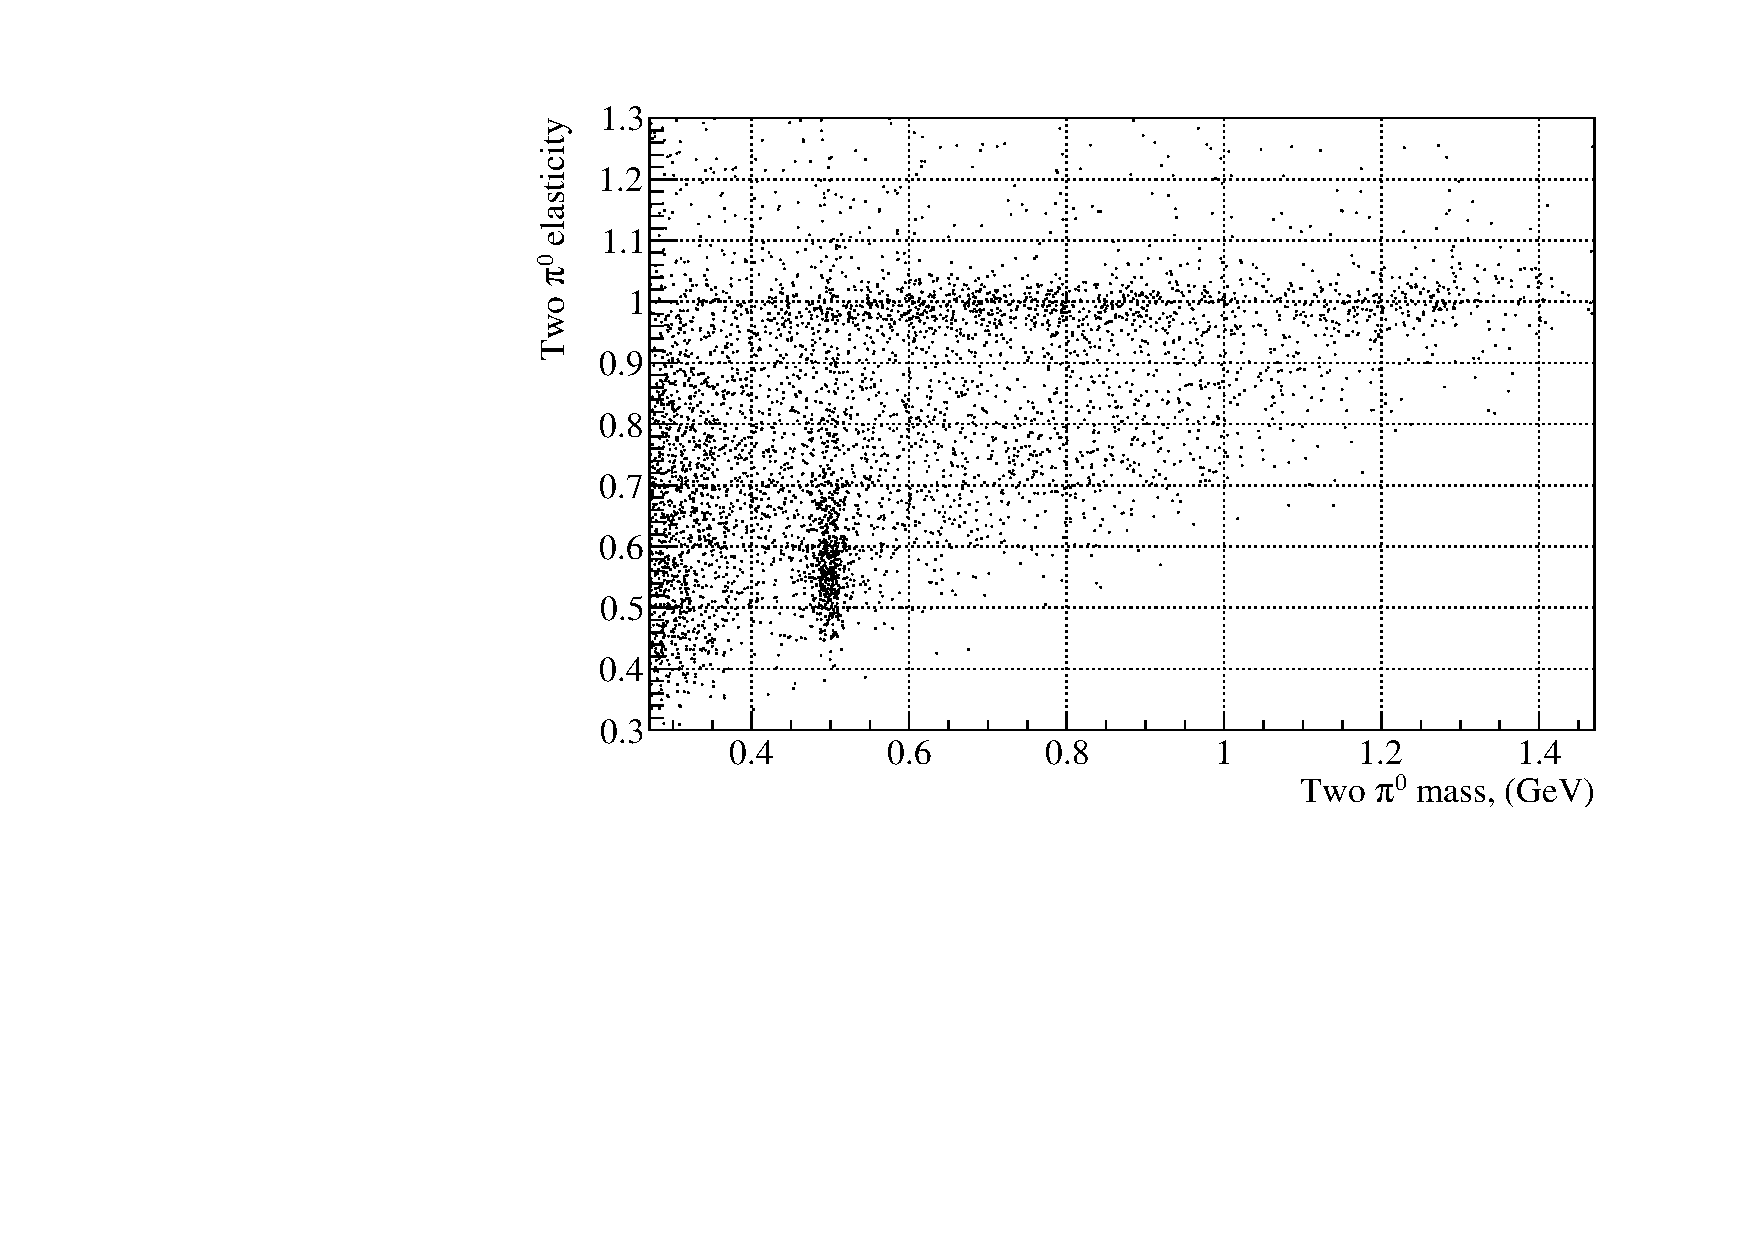
\includegraphics[width=4.75in]{figures/2d_be.pdf}
\caption{Two neutral pion elasticity (ratio of two-pion energy to that expected
  for exclusive production) vs.\ invariant mass of two pions
  for the beryllium target.
\label{fig:2dbe}}
\end{figure}

Including BCAL showers in the neutral pion reconstruction increases
the acceptance (especially for the large invariant mass region) and the number
of observed events goes up by an order of magnitude. For the beryllium target
this increases the number of exclusive events to $\sim 10$~k and for
the helium target to $\sim 200$~k events. Fig.~\ref{fig:bemass}
shows the two $\pi^0$ invariant mass distribution. These data have the BCAL included,
the two-pion energy is required to be within
10\% of that expected for exclusive events, and the production angle
of the two-pion system was required to be below one degree. The $f_2$ meson
peak is clearly seen. Fig.~\ref{fig:beheelast} shows the elasticity
distribution for both helium and beryllium targets with BCAL
reconstruction included (time accidentals and empty target
background subtracted).
\begin{figure}[!h]
\centering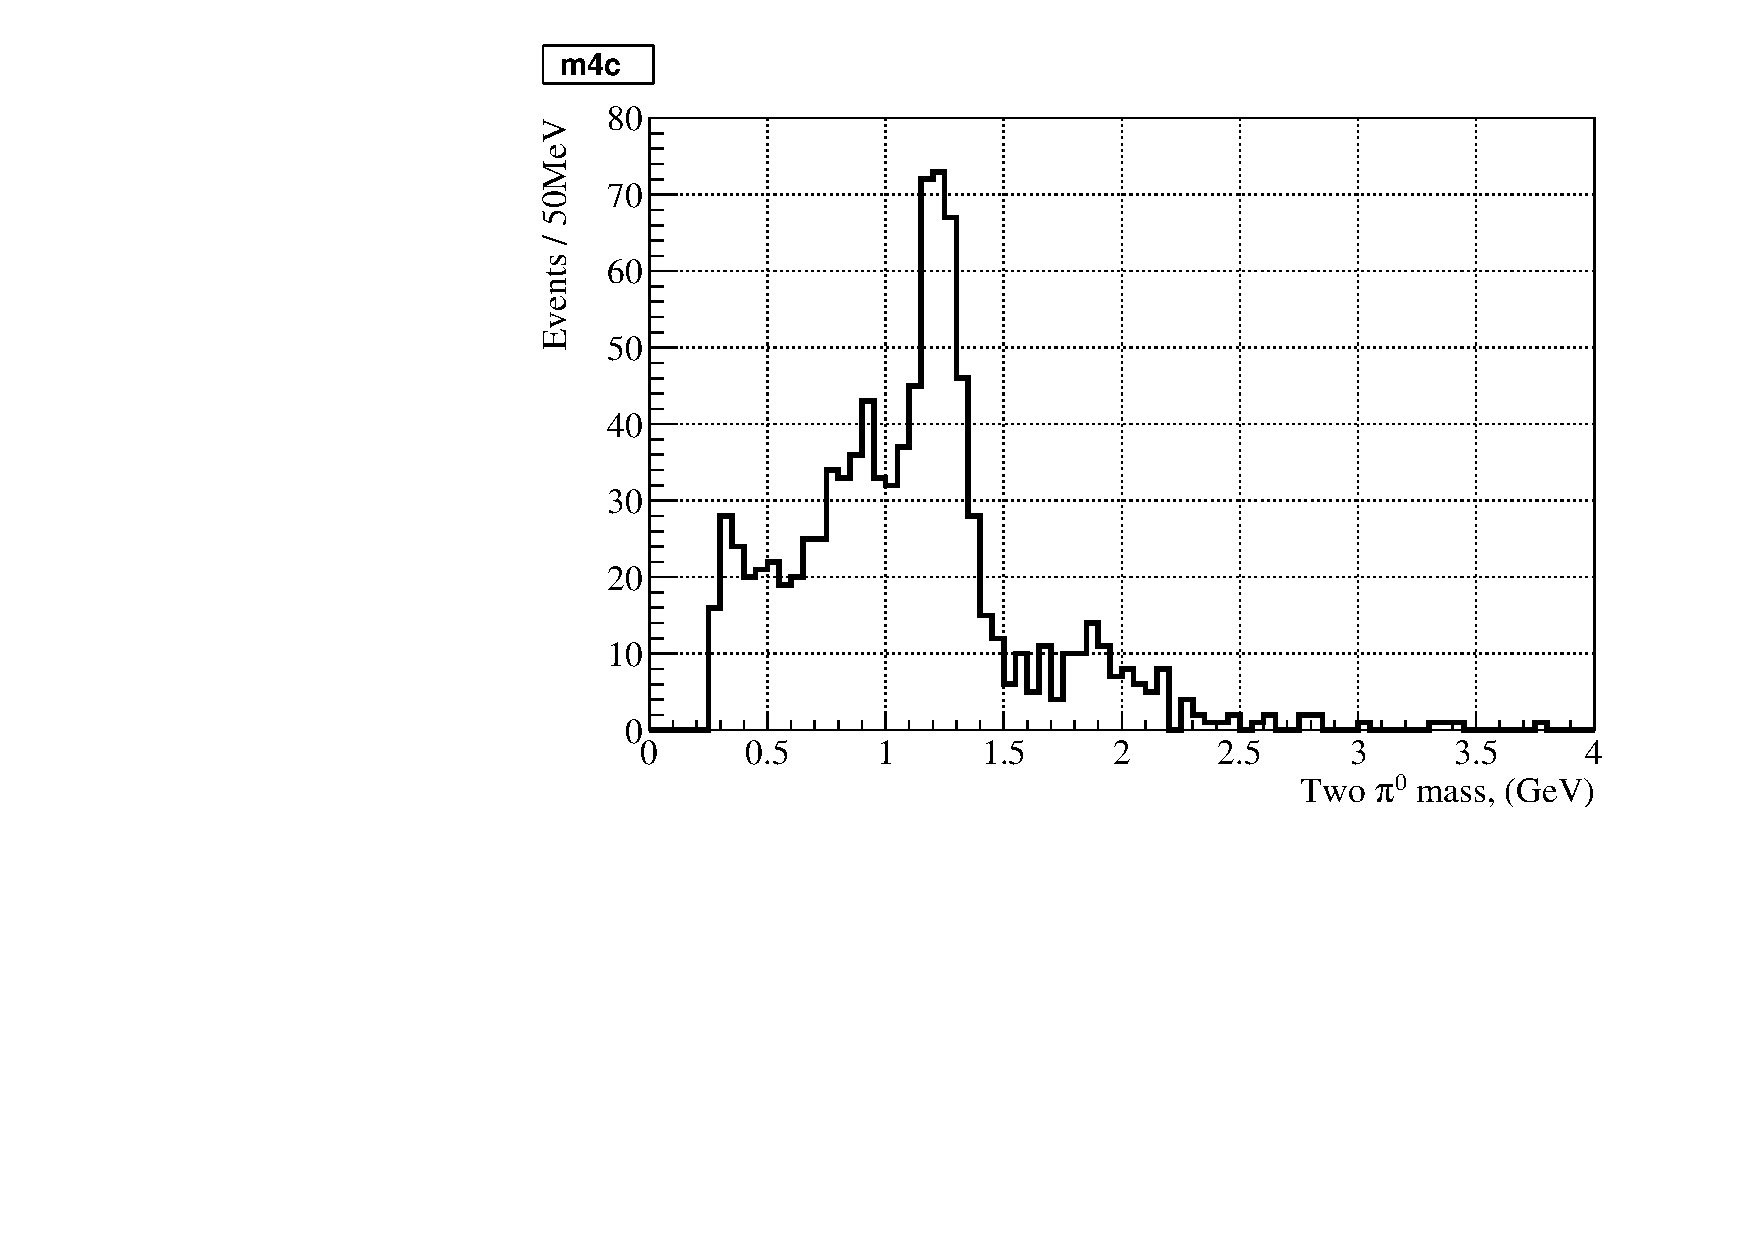
\includegraphics[width=4.75in]{figures/be_mass.pdf}
\caption{Two neutral pion invariant mass for the exclusive events
  (i.e., within 10\% of the expected energy). Data from the beryllium target. The production angle
  was required to be below one degree.
\label{fig:bemass}}
\end{figure}
\begin{figure}[!h]
\centering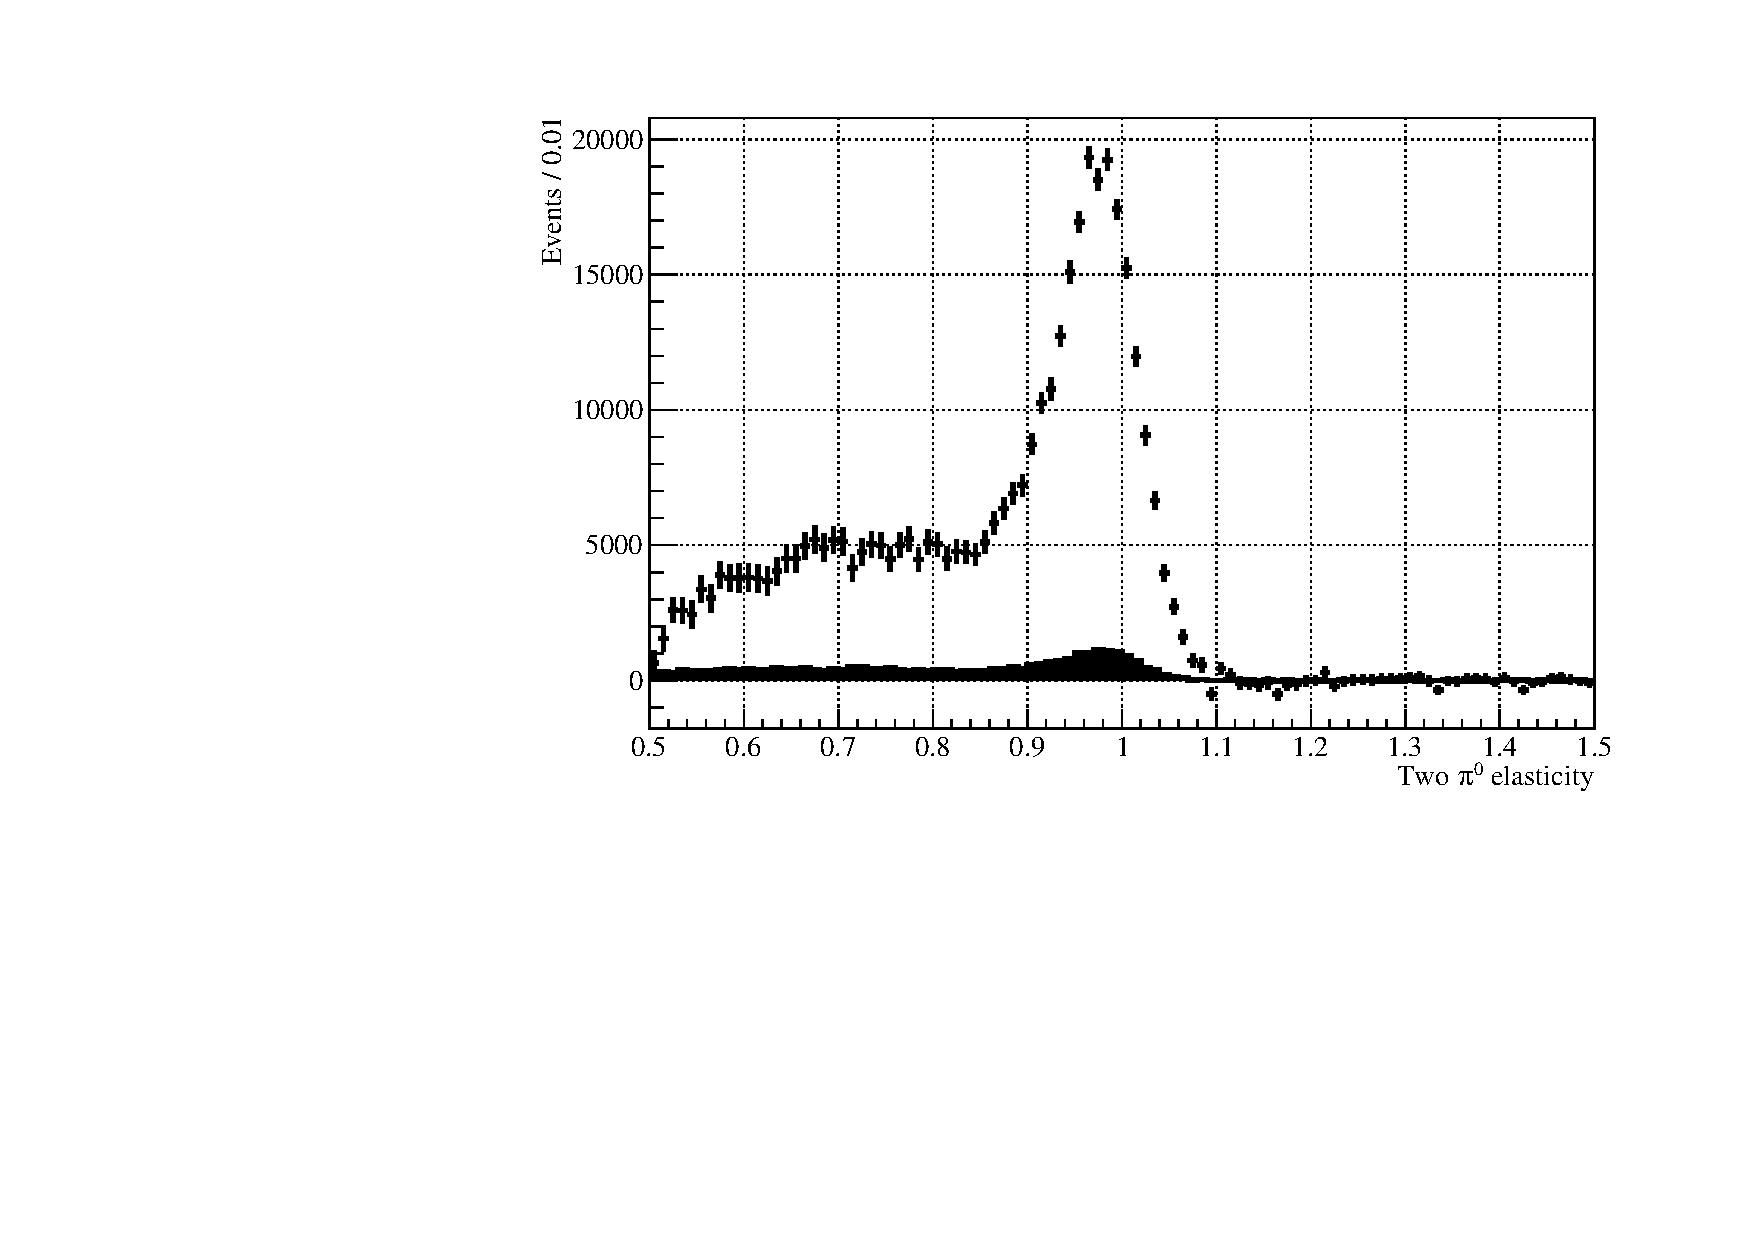
\includegraphics[width=4.5in]{figures/hebe_elast.pdf}
\caption{The two-pion elasticity distribution with BCAL included in the
  analysis. Empty target data and time accidentals are subtracted. Open
  histogram: helium target, $\sim 200$~k events in the elastic
  peak. Solid histogram: beryllium target, $\sim 10$~k events in
  the peak.
\label{fig:beheelast}}
\end{figure}

We wish to highlight the good detector
resolution for two $\pi^0$ production kinematics variables, the
presence of the calibration process ($K_S$) in the data and the
controllable level of backgrounds observed for light nuclear target
exposure.

\section{Photon beam flux}

\subsection{Photon beam flux accounting with the GlueX pair spectrometer}
The photon beam flux can be directly extracted by analyzing the pair
spectrometer (PS) data with the thin beryllium converter installed in
the beam in from of it.  The absolute normalization of the PS
performed with the total absorption counter (TAC) during the dedicated
run.

The systematics from the photon beam flux accounting by pair
spectrometer is originated from few main contributions: overall
spectrometer calibration with TAC quality; accuracy of the Monte-Carlo
simulation of this process; long term stability of the spectrometer
performance; and change of conditions between low intensity beam (TAC
calibration) and production intensity.  There are few other less
significant contributions. GlueX PS acceptance \cite{hdnote3684} shown
on Fig.~\ref{fig:psacc}. For the proposed experiment PS magnetic field
should be reduced to cover the beam energy range $5-6\,GeV$.
\begin{figure}[tpb]
\begin{center}
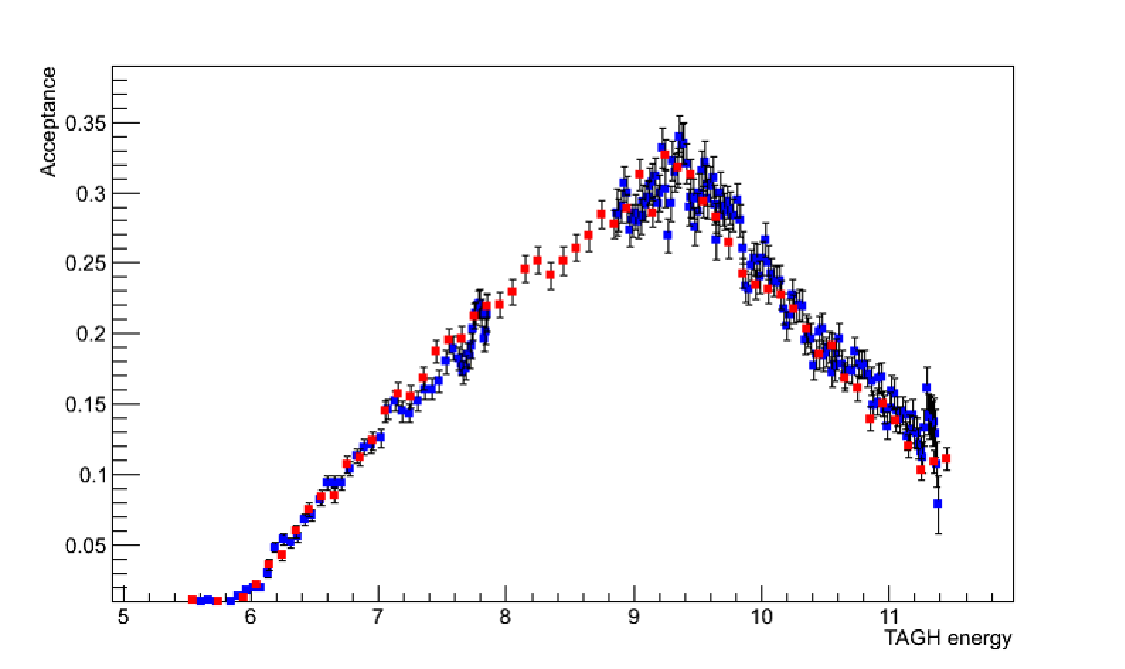
\includegraphics[width=10cm,angle=0]{figures/ps_acceptance.pdf}
\end{center}
\caption{GlueX PS acceptance extracted from TAC data analysis (blue points);
red points -- Monte-Carlo simulation}
\label{fig:psacc}
\end{figure}
The methodology and accuracy of the PS analysis is the same as in
PrimEx-D experiment, currently running in Hall-D, and has value
$\sim1-1.5\,\%$ \cite{PrimexDexp}.

\subsection{Cross section verification with the exclusive single $\pi^0$ photoproduction}
The extracted cross section can also be normalized on or independently
from PS analysis verified with the $\pi^0$ radiative decay width
extraction.  Fig.~\ref{fig:leaddndt} shows exclusive single $\pi^0$
photoproduction yield at forward angle obtained by the PrimEx
experiment and used for $\pi^0$ radiative decay width extraction.
\begin{figure}[tpb]
\begin{center}
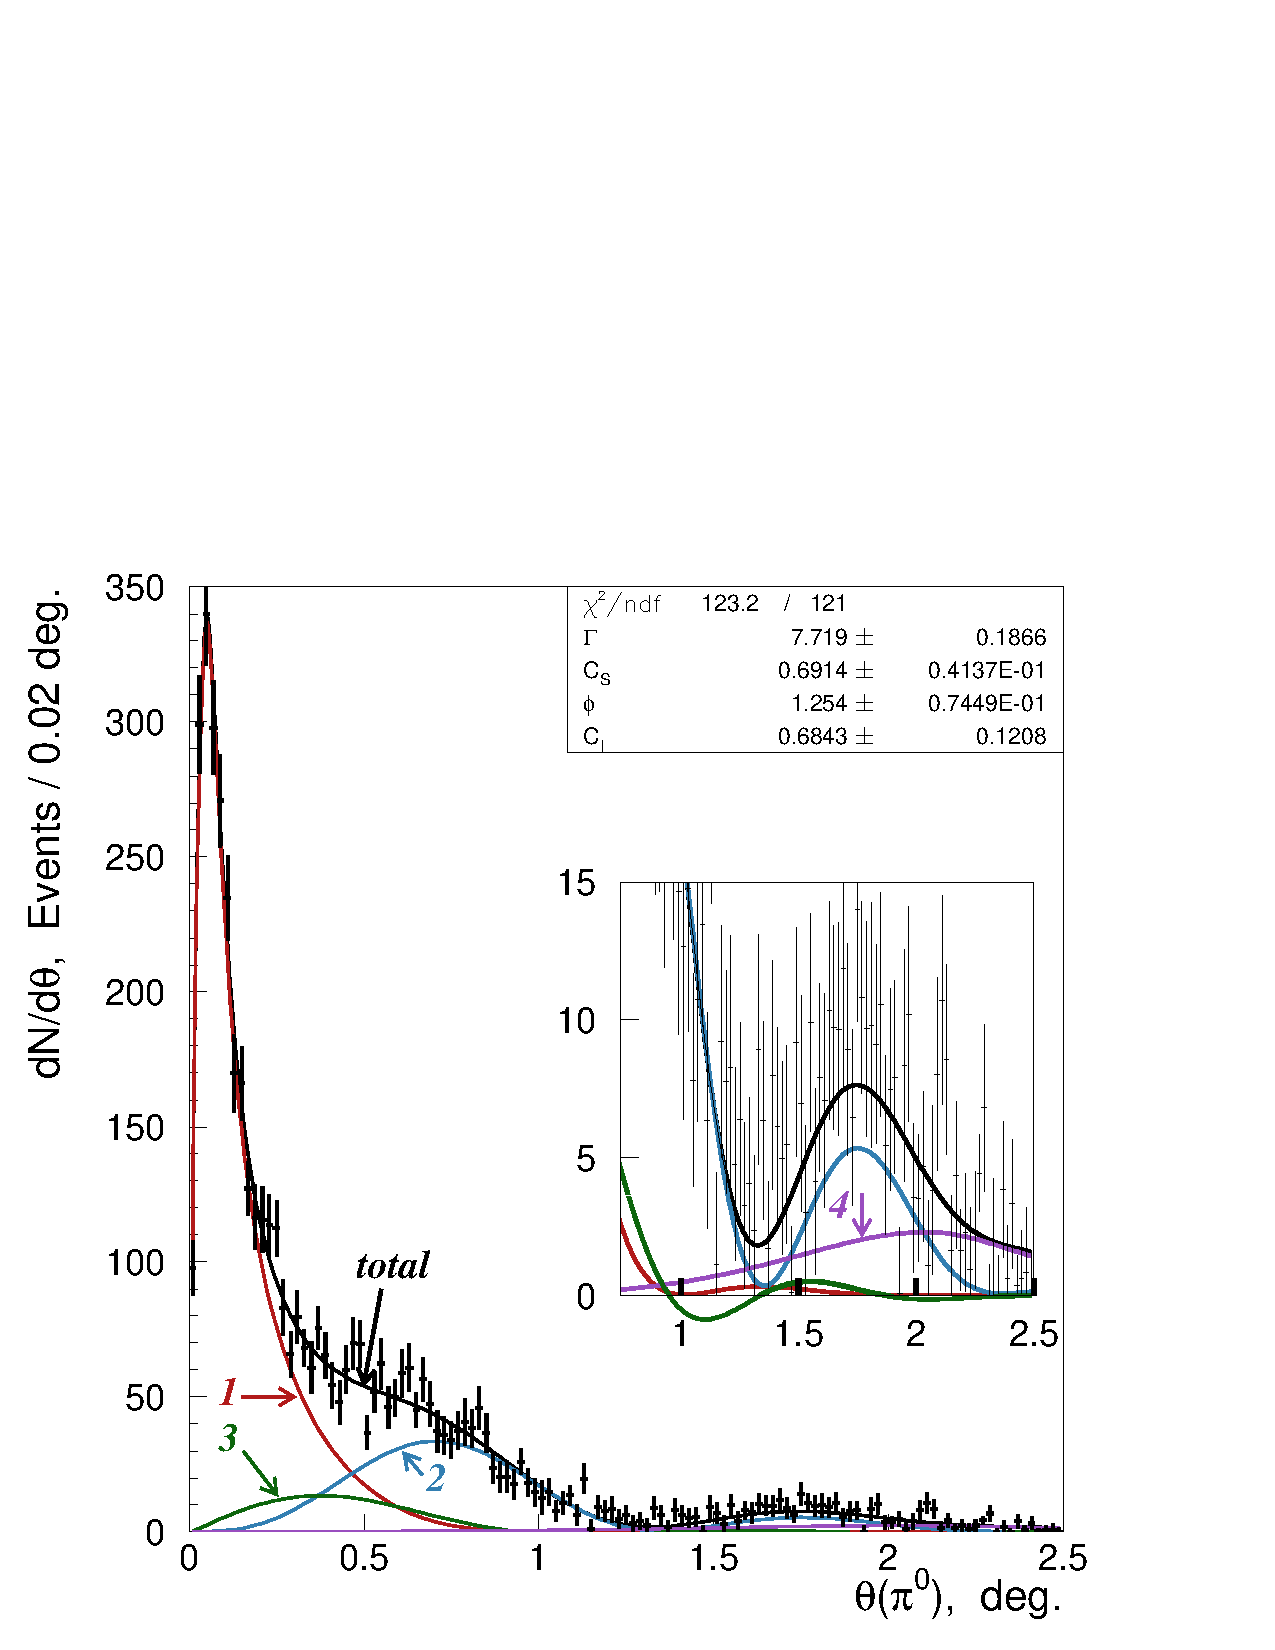
\includegraphics[width=8cm,angle=0,trim={1.5cm 0.5cm 3.5cm 9.5cm},clip]{figures/dndt_pb_partial.pdf}
\end{center}
\caption{Exclusive $\pi^0$ production yield at forward angle on lead target
observed in the PrimEx experiment \cite{Larin:2010kq}. Curves show production mechanisms input:
1 -- Primakoff, 2 -- strong coherent, 3 -- interference of first two mechanisms, 4 -- strong incoherent}
\label{fig:leaddndt}
\end{figure}
The photon beam flux in PrimEx was $0.725\times10^{12}$ for
4.9-5.5$\,$GeV bremsstrahlung spectrum part on 5\% rad. len. lead
target. The distance between calorimiter and target was $\sim7.3\,m$
and the central square part of the calorimeter, used in analysis was
$\sim70\times70\,cm$. These conditions have to be compared with the
proposed experiment conditions: 20 days of $~10^7$ collimated beam
photon/sec (i.e. 20 times more than PrimEx lead target beam flux), the
distance between target and FCAL $\sim6.2\,m$ and active calorimeter
part diameter $\sim2\,m$.  The central hole with one calorimeter
modules layer around which should be excluded from the analysis for
PrimEx case was $\sim8\times8\,cm$ and for FCAL $\sim20\times20\,cm$,
which is decreasing FCAL acceptance at forward angle. Comparison of
these experimental conditions allows us expecting an order of
magnitude higher exclusive single $\pi^0$ photoproduction statistics.
Thus PrimEx statistical uncertainty for lead will be decreased from
$\sim2.5\,\%$ down to $\sim1\,\%$.  For the systematical uncertainty,
in PrimEx it was $\sim2.1\,\%$ and has two major contributions: yield
extraction ($\sim1.6\,\%$) and photon beam flux accounting
($\sim1.0\,\%$).  The first contribution is partly statistically
driven and reduces with increasing of statistics; and the second one
cancels out since it is the same photon beam flux for the single and
double exclusive $\pi^0$ photoproduction.  The main factors increasing
systematics for the proposed experiment are: the angular resolution of
FCAL is about a factor of two worse than for PWO crystals used in the
PrimEx analysis;
%the single $\pi^0$ photoproduction theory needs to be involved since
%the photon beam energy spectra are not the same for PrimEx and
%proposed experiment;
and the magnetic field is not swiping out charged background like it
was in PrimEx.  As a result we can expect slightly worse systematical
uncertainty than in PrimEx and statistical precision of $\sim1\,\%$,
i.e. total error $2.5-3.5\,\%$ for $\pi^0$ radiative width extraction
(excluding absolute photon beam flux accounting, target number of
atoms and partly FCAL trigger efficiency contributions to the
systematics which are canceling out).  The expected total beam flux
uncertainty for such a normalization should also include the PrimEx
total error of the $\pi^0$ radiative width, which was recently
reported as 1.5\% \cite{Larin:2018}.  All this gives $\sim3-4\,\%$
error for photon beam flux from normalization to the re-exctracted
$\pi^0$ radiative decay width.

\subsection{Muon pair production}
In addition to these normalization channels, production of muon pairs,
which has a known cross section, can be used as a measurement of
photon flux. Since the experiment will be running concurrently with
the Charged Pion Polarizability (CPP) experiment, the photon flux on
target will be the same by definition. CPP plans to use muon pair
creation by beam photons as its main normalization channel, and so
those measurements will be available for normalization of the neutral
pion channel as well. In the case of CPP, the GlueX track finding and
fitting efficiency will have to be determined for muon pairs, but any
systematic error in that determination will largely cancel when
applied to charged pion pairs. That will not be the case for the
neutral pion channel and will have to be taken into account when
evaluating systematic errors due to this method of normalization. In
any case, muon pair production should provide a useful check on the
other methods mentioned above.

\section{Errors and Sensitivity}
We summarize the anticipated errors in the determination of the $\pi^0$ polarizability. We assume 
20 days of running on a 5\% radiation length $^{208}$Pb target, 10$^7$ photons/s, and nominal acceptance for $\pi^0 \pi^0$.
Table \ref{errors} summarizes the estimated statistical and systematic errors. In the following we describe each of
these contributions in detail: 

%\end{landscape}
% \begin{landscape}
\begin{table}[bt]
\caption{Uncertainties in the extraction of $\pi^0$ polarizabilities $\alpha_{\pi^0}-\beta_{\pi^0}$.
\label{errors}
}
\begin{center}
\begin{tabular}{|l|l|c|c|}
\hline
\hline
  &  Source  & Uncertainty   \\  \hline \hline
  1 & Statistical uncertainty  &  2.3 \%    \\ \hline
  2 & Flux normalization &  1.5 \%     \\ \hline
  3 & Signal extraction  & 3.0 \%  \\ \hline
  4 & Detector acceptance and efficiency &  3.5 \%   \\ \hline
  5 & Total systematic error  &  4.8\% \\ \hline
  6 & Total error on cross section  &  5.3\% \\ \hline
  7 & Projected error in $\alpha - \beta$ &  41\%  \\ 
 \hline
 \hline
\end{tabular}
\end{center}
\end{table}
%\end{landscape}

\begin{enumerate}

\item
Statistical uncertainty in extraction of the Primakoff signal as determined by the fit shown in the top left plot in Fig.\,\ref{fig:decomposition_PrimNCICeta} (Section\,\ref{sec:signalfit}).

\item
Flux normalization. We have several methods for determining the flux (Section\,\ref{sec:flux}). The Primex-D experiment expects an uncertainty of 1.5\% and we use that as our estimate here.

\item
Systematic uncertainty in extraction of the signal. This contribution is estimated to be 3\% based on differences obtained in the Primakoff signal by varying the amount of background contributions (Section\,\ref{sec:signalfit}).

\item
Detector acceptance and efficiency. We can measure the detector acceptance times efficiency for the process $\gamma \mathrm{Pb} \rightarrow \pi^0 \mathrm{Pb}$ with an accuracy of 3.5\% (Section\,\ref{sec:pi0norm}), which
should allow us to reduce the systematic uncertainty in the acceptance calculation for the process of interest to this level.

\item
Total systematic error (items 2-4): combining the systematic errors in quadrature gives 4.8\%.

\item 
Error on cross section (quadrature sum of items 1 and 5): 5.3\%.

\item
The current estimate by Dai and Pennington (Table II in Ref.\,\cite{Dai:2016ytz}) indicates
that a 13\% determination of
$\sigma(\gamma\gamma\rightarrow\pi^0\pi^0)$ will determine the
combination $\alpha_{\pi^0}-\beta_{\pi^0}$ to a precision of 100\%, i.e., $\Delta(\alpha_{\pi^0}-\beta_{\pi^0}) \sim 7.7\Delta(\sigma$) .
From here we estimate that our uncertainty on $\Delta(\alpha_{\pi^0}-\beta_{\pi^0}) \sim$ 41\%. We note that the basis for extracting the polarizabilities may be improved
in the near future and theoretical effort is being directed specifically toward this goal.

\end{enumerate}

\begin{table}[hbt]
\caption{Approved beam request and running conditions for CPP. NPP would run concurrently.
\label{request}
}
\begin{center}
\begin{tabular}{|l|c|c|c|c|c|c|c|c|}
\hline
\hline
  Running condition  &            \\ \hline
  Days for production running  &   20   \\ \hline
  Days for calibrations &  5       \\ \hline
  Target   & $^{208}$Pb   \\ \hline
  Photon intensity in coherent peak &   10$^7$ photons/s     \\ \hline
  Edge of coherent peak  &  6 GeV   \\ \hline
 \hline
 \hline
\end{tabular}
\end{center}
\end{table}
 
\section{Summary and beam request}
We have investigated the possibility of determining the neutral pion
polarizabilities $\alpha_{\pi^0}-\beta_{\pi^0}$, a quantity for which there are no existing measurements.
Our proposal is to extract the polarizability from a 
measurement of the cross section of the Primakoff reaction $\gamma
\rm{Pb}\rightarrow \pi^0 \pi^0 \rm{Pb}$. We propose to make this
measurement using data taken simultaneously with the CPP\cite{CPPexp}
experiment in Hall D. Table \ref{request} summarizes the approved beam request for the CPP experiment.
The existing GlueX detector has sufficient
resolution and high acceptance for this process. We expect to collect approximately 2500 signal events during the
approved 20 PAC days. The anticipated statistical uncertainties on
the signal represent a significant improvement over existing data as shown in Fig.\,\ref{fig:sigma_2pi0_figs_4}.
Using the estimate by Dai and Pennington \cite{Dai:2016ytz} we expect to be able to make the first extraction of the 
$\alpha_{\pi^0}-\beta_{\pi^0}$ polarizability with an uncertainty of 49\%.

\begin{figure}[tpb]
\centering
\includegraphics[page=4,width=4.75in]{figures/sigma_2pi0_figs.pdf}
\caption{Estimated statistical uncertainties on determining $\sigma(\gamma\gamma\rightarrow\pi^0\pi^0$) during 20 PAC days running simultaneously with the approved CPP experiment. The data points from the single previous Cristal Ball measurement \cite{Marsiske:1990hx} are shown for comparison.
\label{fig:sigma_2pi0_figs_4}}
\end{figure}






%\input{JLAB_MuonDetector.tex}



%---------------------------------------------------------------------------------------------------------------
%--------------------------------- References-----------------------------------------------------------------
%---------------------------------------------------------------------------------------------------------------
\clearpage

%\nocite{*}
\bibliographystyle{unsrt}                                                                              
\bibliography{Pi0Polarizability}   

\newpage
\appendix

\def\red{\color{red}}
\def\blue{\color{blue}}
\def\green{\color{green}}
\def\violet{\color{violet}}
\def\orange{\color{orange}}
\newcommand{\fr}{\frac}
\newcommand{\beq}{\begin{equation}}
\newcommand{\eeq}{\end{equation}}
\newcommand{\bea}{\begin{eqnarray}}
\newcommand{\eea}{\end{eqnarray}}
\newcommand{\zero}{{(0)}}
\newcommand{\one}{{(1)}}
\newcommand{\eps}{\epsilon}
\newcommand{\ord}[1]{{\cal{O}}( #1 )}
\newcommand{\B}{{\bf B}}
\newcommand{\Bdag}{{\bf B^\dagger}}
\newcommand{\cgsu}[3]{ \langle #1 #2 \mid #3\rangle}
\newcommand{\water}[2]{ #1,$^2$,#2}
\def \ba{\begin{eqnarray}}\def\ea{\end{eqnarray}}
\def\bc{\begin{center}}\def\ec{\end{center}}
\def\nn{\nonumber\\}\def\v{\vec}

\section{More on theoretical predictions}

The scattering amplitude for $\gamma\gamma^*\to\pi^0\pi^0$ is given in
terms of the Compton tensor, whose low energy expansion in the Compton
scattering channel $\gamma\pi^0\to\gamma\pi^0$ is given in terms of
the electric and magnetic polarizabilities of the $\pi^0$. For the
case of interest with one real photon, the Compton tensor is given in
by two amplitudes, namely:
   
   \bea
   T_{\mu\nu}&=&-(A(s,t,u)+\frac 14 B(s,t,u)) (\frac 12\, s \;g_{\mu\nu}-k_\nu q_\mu)\\
   &+&\frac{1}{4s} B(s,t,u)  ( (s-q^2) p_{-\mu} p_{-\nu}-2(k\cdot p_-\; q_\mu p_{-\nu}+q\cdot p_{-} k_\nu p_{-\mu}-g_{\mu\nu} k \cdot p_-\; \;q\cdot p_-)
   \eea

Here $s=W_{\pi\pi}^2$ is the invariant mass squared of the two
$\pi^0$s, $k$ the momentum of the beam photon, $q$ the momentum of the
virtual photon, and $p_-$ the $p_-=p_1-p_2$ the momentum difference
between the two pions.
  
  The limit of interest for the polarizabilities is:
  \bea
 \alpha_{\pi}&=& - \frac{\alpha}{2 M_\pi}  (A(s,t,u)-\frac 2 s M_\pi^2 B(s,t,u))\arrowvert_{s=0, t=u=M_\pi^2}\nonumber\\
 \beta_{\pi}&=&
  \frac{\alpha}{2 M_\pi} A\arrowvert_{s=0, t=u=M_\pi^2}
  \eea
  where $ \alpha_{\pi}$ $ \beta_{\pi}$ are the electric and magnetic polarizabilities respectively.
  
The low energy limit is analyzed in ChPT. At the lowest significant
order, i.e., one loop, the $\pi^0$ polarizabilities are entirely given
in terms of known quantities, namely:
\bea
\alpha_{\pi_0}&=&-\beta_{\pi_0}= -\frac{\alpha}{96 \pi^2 M_\pi F_\pi^2}\simeq -0.55\times 10^{-4}~{\rm fm}^3
\eea
The positive magnetic susceptibility indicates that the $\pi_0$ is
diamagnetic, and naturally the negative electric polarizability tells
that it behaves as a dielectric.

There are higher order corrections in the chiral expansion to the
above prediction corresponding to a two-loop calculation, which is
undefined up to two low energy constants $h_\pm$ in the notation of
Ref. \cite{Bellucci:1994eb}, expected to be significant for the
corrections.

The amplitudes $A$ and $B$ are constrained by unitarity and
analiticity to satisfy dispersion relations. In particular below
$s\sim 0.8\text{ GeV}^2$ the dominant contributions are for the pair
of pions in an S-wave. The rather well established S-wave phase shifts
thus allow for implementing dispersion
relations \cite{Donoghue:1993kw,
Oller:2008kf,Moussallam:2013una,Dai:2014zta,Dai:2014lza,Dai:2016ytz}.
In this proposal the model by Donoghue and
Holstein \cite{Donoghue:1993kw} for implementing the dispersive
representation using S-wave final state interaction was adopted. The
model implements twice subtracted dispersion relations for the isospin
0 and 2 components of the amplitude A with the addition of t- and
u-channel resonance exchanges for both A and B. The four subtraction
constants require the experimental input of the cross section to be
measured by the proposed experiment.

A summary of useful  theory results is the following:  

1) representation of the Compton amplitudes:
\bea
s\;A(s,t,u)&=& -\frac 23(f_0(s)-f_2(s))+\frac 23 (p_0(s)-p_2(s))-\frac s 2\sum_{V=\rho,\omega} R_V (\frac{t+M_\pi^2}{t-M_V^2}+\frac{u+M_\pi^2}{u-M_V^2})\nonumber\\
B(s,t,u)&=&-\frac 18 \sum_{V=\rho,\omega} R_V (\frac{1}{t-M_V^2}+\frac{1}{u-M_V^2})\nonumber\\
R_V&=&\frac{6 M_V^2}{\alpha} \frac{\Gamma(V\to \pi \gamma)}{(M_V^2-M_\pi^2)^3}
\eea
where $V=\rho,\;\omega$, 
\bea
p_I(s)&=& f_I^{\rm Born}(s)+p_I^A(s)+p^\rho_I(s)+p_I^\omega(s)\nonumber\\
p_0^A(s)=p_2^A(s)&=&\frac{L_9^r+L_{10}^r}{F_\pi^2}\left(s+\frac{M_A^2-M_\pi^2}{\beta(s)}\log\frac{1+\beta(s)+s_A/s}{1-\beta(s)+s_A/s}\right)\nonumber\\
p_0^\rho(s)&=&\frac 32 R_\rho\left( \frac{M_\rho^2}{\beta(s)}  \log\frac{1+\beta(s)+s_\rho/s}{1-\beta(s)+s_\rho/s}\right)\nonumber\\
p_2^\rho(s)&=&0\nonumber\\
p_0^\omega(s)=-\frac 12 p_0^\omega(s)&=&-\frac 12 R_\omega\left( \frac{M_\omega^2}{\beta(s)}  \log\frac{1+\beta(s)+s_\omega/s}{1-\beta(s)+s_\omega/s}-s\right),
\eea
where $\beta(s)=\sqrt{\frac{s-4 M_\pi^2}{s}}$, $M_A$ the mass of the $A_1$ resonance. The $f_I$s are given by the dispersive representation:
\bea
f_I(s)&=& p_I(s)+\Omega_I(s)\left(c_I+d_I\;s-\frac{s^2}{\pi} \int_{4M_\pi^2}^\infty p_I(s') \text{Im}(\Omega_I^{-1}(s'))\frac {ds'} {(s'-s) s'^2}\right),
\eea
with the Omn\`es function:
\bea\Omega_I(s>4 M_\pi^2)&=&e^{i\phi_I(s)} \exp\left(\frac s\pi\int_{4 M_\pi^2}^\infty \frac{\phi_I(s')-\phi_I(s)}{s'-s} \frac{ds'}{s'}+\frac{\phi_I(s)}{\pi}\log\frac{4M_\pi^2}{s-4M_\pi^2}\right).
\eea
the phases $\phi_I$ are related to the corresponding $\pi\pi$ S-wave phase shifts according to:
\bea
\phi_0(s)&=&\theta(M-\sqrt{s}) \delta_0^0(s)+\theta( \sqrt{s}-M)(\pi-\delta_0^0(s))\nonumber\\
\phi_2(s)&=&\delta_0^2(s),
\eea
where $M$ is the mass of the $f_0$ resonance.  

The values used for the parameters entering the representations above are:
\bea
L_9^r+L_{10}^r&=&1.43\pm 0.27\times 10^{-3}\nonumber\\
s_i&=&2 (M_i^2-M_\pi^2)\nonumber\\
R_\omega&=& 1.35/\mathrm{GeV}^2;~~~R_\rho=0.12/\mathrm{GeV}^2
\eea

and the $\pi\pi$ phase shifts are well approximated up to $\sqrt{s}\sim 1.5~\mathrm{GeV}$ by the parametrization:
\bea
\delta_0^I(s)&=& \arcsin\left(\frac{\Gamma_I}{2\sqrt{(\sqrt{s} - M_I)^2 +\frac{ \Gamma_I^2}{4}}}\right)+\sum_{n=0}^N a_n\;\, (\sqrt{s})^n
\eea
where we include one single resonance for each $I=0,2$.

For the available data we need only up to $N=3$ for $I=0$, with the result:
\bea
M_0=0.994~\mathrm{GeV};&&\Gamma_0=0.0624~\mathrm{GeV}\nonumber\\
a_0=-1.439;&&a_1=6.461 /\mathrm{GeV};~~a_2=-5.529 /\mathrm{GeV}^2;~~a_3=2.022 /\mathrm{GeV}^3
\eea
For the case $I=2$ one finds that   the resonance term is not needed at all and a good fit is provided with $N=3$ with the result:
\bea
a_0=-0.878;&&a_1=-0.611 /\mathrm{GeV};~~a_2=-0.083 /\mathrm{GeV}^2;~~a_3=0.115 /\mathrm{GeV}^3
\eea


The $\gamma\gamma\to\pi_0\pi_0$ in the S-wave approximation
valid up to about $\sqrt{s}\sim 0.9~\mathrm{GeV}$ is given by:
\bea
\sigma_{\gamma\gamma\to\pi^0\pi^0}(|\cos \theta|<Z)(s)&=&\frac{\pi \alpha_{EM}^2}{s^2}
\frac Z2  \sqrt{s (s -4 M_\pi^2)} \\
&\times&(\mid A(s) s-M_\pi^2  B(s)\mid^2\nonumber\\
&+&\frac {1}{s^2} \left(M_\pi^4- \frac{1}{16}(\frac{Z^2}{3} s(4 M_\pi^2-s)+4(s-2 M_\pi^2)^2)\right)\mid B(s)\mid ^2) \nonumber
\eea
 Fitting to the Cristal Ball data\cite{Marsiske:1990hx} the parameters $c_0,\;d_0,\;c_2,\;d_2$ can be estimated,  giving in the corresponding units: 
\bea
c_0&=& -0.529 \nonumber\\
d_0&=&-2.033 \nonumber\\
c_2&=& 0.953\nonumber\\
d_2&=& -1.271.
\eea

\section{Parameterization of the nuclear coherent production  \label{sec:NCsigma}}
We consider the reaction $\gamma A \rightarrow m_{\pi\pi} A$, where $m_{\pi\pi}\rightarrow \pi\pi$ is a dipion system.
The $2\pi$ system is treated as a particle with mass $m_{\pi\pi}$, which is produced with  four-momentum transfer $t$.  
The cross section for a three-body final state can be written as \cite{BNLQGS020900}:
\begin{eqnarray}
d\sigma & = & \frac{1}{4\mathcal{F}} \, d\phi_3 \, |\mathcal{A}|^2 \\
\mathcal{F} & = & p_\gamma^{cm} \sqrt{s} \\
d\phi_3 & = & \frac{4}{(4\pi)^5} {p_\sigma^{cm} \over \sqrt{s}} d\Omega_\sigma^{cm}\, p_\pi^{\sigma} dm_{\pi\pi} d\Omega_\pi^{\sigma} \\
{dt \over d\Omega_\sigma^{cm} } & = & {dt \over d\cos{\theta}_\sigma^{cm} d\phi_\sigma^{cm} } = {2\, p_\gamma^{cm} p_\sigma^{cm}  \over d\phi_\sigma^{cm} }
\end{eqnarray}
The center-of-mass energy (cm) energy and the momentum transfer are represented by the commonly used variables $s$ and $t$. 
%The invariant mass of the 2$\pi$ system ($\sigma$) is denoted by W$_{\pi\pi}$. 
Other variables are subscripted by particle name and their superscripts indicate the reference frame. Thus $p_\gamma^{cm}$ is the incident photon momentum, $p_\sigma^{cm}$ is the scattered momentum,  and $\Omega_\sigma^{cm}$ corresponds to the solid angle of the $\sigma$, all in the cm frame.  
The momentum of the pions in the $\sigma$ rest frame is denoted by $p_\pi^{\sigma}$ and $\Omega_\pi^{\sigma}$ denotes the solid angle of  one of them.
Thus the cross section can be written as
\begin{eqnarray}
{d\sigma \over dt dm_{\pi\pi} d\phi_{\sigma}^{cm} d\Omega_\pi^{\sigma} } & = & {1 \over 2(4\pi)^5} {p_\pi^\sigma \over (p_\gamma^{cm})^2 s } |\sum_i \mathcal{A}^i|^2 ,     \label{eq:sigma_phi3}
\end{eqnarray}
where the index $i$ runs over the number of resonances or mechanisms included in the calculation. We  will assume that we can parameterize each production amplitude as a factorized product
\begin{eqnarray}
\mathcal{A}^i & = & \mathcal{A}_t(t)^i \, \mathcal{A}_W(m_{\pi\pi})^i \, \mathcal{A}_\tau(\Phi, \phi, \theta)^i.
\end{eqnarray}
For simplicity, we will drop the superscript $i$ since for the moment we are considering  single production mechanism.
The function $\mathcal{A}_\tau(\phi_{\pi\pi}, \phi_\pi, \theta_\pi)$ contains the angular dependence of the produced pions, 
where\,($\theta_\pi,\phi_\pi$)  are the decay angles in the rest frame of the $2\pi$ system, which is flat for S-wave production. 
Azimuthal symmetry is broken by the photon polarization, where $\phi_{\pi\pi}$\,is the angle between the plane of photon polarization and the production plane. The amplitudes are
given by Eq.\,\ref{eq:PhiAmplitude} and lead to a cross section dependence of the form $\mathcal{A}_\tau \propto (1 + \mathcal{P} \cos{2\phi_{\pi\pi}}$). 

The primary background in this mass region is given by the 
f$_0(500)(J^{PC}=0^{++})$  also called the $\sigma$. The $\sigma$ has the same angular structure as the Primakoff 
reaction and can only be identified through its dependence on $t$ and $m_{\pi\pi}$.
Our parameterization of the mass dependence for the $\sigma$ meson is described in Section\,\ref{sec:ParmSwave}.

We assume the $-t$ dependence of the $\sigma$ has a similar form as for single $\pi^0$ production, namely $\mathcal{A}_t(t) \propto \sin{\theta_{\pi\pi}} \times F_{st}(t)$.  The $\sin{\theta_{\pi\pi}}$ 
comes from the spin-flip required at forward angles to produce a $0^+$ system from a spin-zero target. The factor $F_{st}(t)$ is the strong form factor for the target, which is approximated to
match calculations for the single $\pi^0$ production (Fig.\,6 from Ref.\cite{Gevorkyan:2009ge}). 



 
\subsection{Parameterization of the s-wave amplitude \label{sec:ParmSwave}}
There is considerable strength in the $2\pi$ channel coming from s-wave production, which is due to the now established $f_0(500)$ meson. It is also commonly referred to as the $\sigma$ 
meson. We assume the amplitude for $\sigma$ production  
is governed by the $\pi\pi$ J=0, I=0 phase shifts. We parameterize the $m_{\pi\pi}$ dependence as 
\begin{eqnarray}       
\mathcal{A}_W(m_{\pi\pi}) & \sim & \frac{m_{\pi\pi}}{2k} \sin{\delta_0} e^{i\delta_0} \left(\alpha_1 + \alpha_2 m_{\pi\pi}^2 \right) + 
 \cos{\delta_0} e^{i\delta_0} \left(\alpha_3 + \alpha_4 m_{\pi\pi}^2 \right),                    \label{eq:Aw}
\end{eqnarray}
where $\delta_0$ is the s-wave phase shift for $I=0$ and $\alpha_i$ (i=1, 2, 3, 4) are empirical constants to be obtained from data.
The first term is due to ``compact source'' production of the pion pair 
(see Eq.\,5 from Ref.\,\cite{Pelaez:2015qba}) and the second term is due to 
production due to an ``extended source,'' for example pion rescattering (see Eq.\,5 from Ref.\,\cite{Bibrzycki:2018pgu} and Eq.\,9 from Ref.\,\cite{Aitchison:1977sm}).  
We use the parameterization for the s-wave phase shifts 
from Appendix D of Ref.\,\cite{Ananthanarayan:2000ht}:\footnote{See also Eq.\,44 of Ref.\,\cite{Pelaez:2015qba}.}  
\begin{eqnarray}  
\tan{\delta_0} & = &  \frac{2k}{m_{\pi\pi}} \left(A_{0}^0 + B_{0}^0 k^2 + C_{0}^0 k^4 + D_{0}^0 k^6 \right) \left(4m_\pi^2 - s_{0}^0 \over M_{\pi\pi}^2 - s_{0}^0 \right), 
\end{eqnarray}
where we use the same notation as the reference with $A_{0}^0$ =0.225, $B_{0}^0$ =12.651\,GeV$^{-2}$, $C_{0}^0$= -43.8454\,GeV$^{-4}$,   $D_{0}^0$=-87.1632\,GeV$^{-6}$, and $s_0^0$=0.715311\,GeV$^2$.
We have converted the constants to units of GeV and evaluated the parameters for $a_0^0=0.225\,m_\pi^{-1}$, and $a_0^2=-0.0371\,m_\pi^{-1}$. These fits are only valid below $m_{\pi\pi}<$ 0.9 GeV because
they do not properly include the $f_0(980)$. 

The empirical constants in Eq.\,\ref{eq:Aw} were determined by fitting $|\mathcal{A}_W|^2$ to the S-wave contribution to the photoproduction 
cross section\footnote{The data are available through the Durham HEP Databases, http://durpdg.dur.ac.uk/.}  
measured by CLAS for $E_\gamma=3-3.8$ GeV \cite{Battaglieri:2009aa} for $-t=0.4-0.5$ GeV$^2$. The fits are for $m_{\pi\pi}=0.3-0.95$ GeV, which is our region of interest.
All four parameters are needed to obtain a good representation to the central values of the data, although the uncertainty band in the data allow for a wide range of parameters. 
Assuming that the constants are real and relatively independent of energy and $-t$,
we take the average of the fitted constants for our parameterization ($\alpha_1=8.4\pm1.4$,  $\alpha_2=-4.1\pm2.2$,  $\alpha_3=2\pm1.1$,  $\alpha_4=8\pm1.1$).

\section{Angular distribution in the helicity basis}

\subsection{Photon density matrix in the helicity basis}
The linear polarization of the photon can be expressed as (Ref.\cite{Schilling:1969um}  Eq. 18-19):
\begin{eqnarray}
\rho(\gamma) & = & \textstyle{1 \over 2} I + \textstyle{1 \over 2} \vec{P_{\gamma}} \cdot \vec{\sigma}, \, \rm{where} \label{eq:photon_sdmH} \\
\vec{P_\gamma} & = & \mathcal{P} (-\cos 2\phi_{\pi\pi}, -\sin 2\phi_{\pi\pi}, 0)
\end{eqnarray}
and $\vec{\sigma}$ are the Pauli matrices. The angle $\phi_{\pi\pi}$ is the angle between the polarization vector of the photon and the production plane and $\mathcal{P}$
represents the degree of linear polarization. Multiplying out these factors gives the expression for the 
photon density matrix in the helicity frame as (Ref.\cite{Salgado:2013dja}  Eq. 219):
\begin{eqnarray}
\rho_{\epsilon,\epsilon'} (\gamma) & = & \textstyle{\frac{1}{2}} \left( \begin{array}{cc} 1 & -\mathcal{P}e^{-2i\phi_{\pi\pi}} \\
-\mathcal{P}e^{2i\phi_{\pi\pi}} & 1 \end{array} \right)    \label{eq:dm_photon}
\end{eqnarray}

\subsection{Parity constraints  \label{sec:parity}}
We consider the reaction $a + b \rightarrow c + d$, where the spin of each particle is denoted by $s_j$, their helicity by $\lambda_j$ and their intrinsic parity by $\eta_j$. 
If parity is conserved, there are relations between amplitudes with opposite helicities, which are  given in Jacob and Wick \cite{Jacob:1959at} Eq. 43 and  Ref.\cite{Schilling:1969um}  Eq. 20 \footnote{We thank Adam
Szczepaniak for clarifying the connection between these papers.} (see also Ref. \cite{leader} Eq. 4.2.3):
\begin{eqnarray}
^{\lambda_a}V_{\lambda_c}^{\lambda_{d}\lambda_{b}}  & = & \left( \eta_c \eta_d \over \eta_a \eta_b \right) (-1)^{s_c+s_d-s_a-s_b} (-1)^{(\lambda_c-\lambda_d)-(\lambda_a-\lambda_b)}  \hspace{0.25cm} ^{-\lambda_a}V_{-\lambda_c}^{-\lambda_{d}-\lambda_{b}}   \label{eq:parity}
\end{eqnarray}

\subsection{S-wave production}
For the case of S-wave production of two pions via the $f_0(500)$ or $\sigma$ meson off an spinless target we have the following constraint:
\begin{eqnarray}
^{\lambda_\gamma}V_{\lambda_\sigma}^{\lambda_{Z}\lambda_{Z}} & = & ^{\epsilon}V_{0}^{00} = \left( \eta_c+ \over -+ \right) (-1)^1 (-1)^{-1} \,\,^{-\epsilon} V_0^{00} = - \eta_c\,^{-\epsilon}V_0^{00}
\end{eqnarray}
For convenience, we have separated out the parity of the scattered state $\eta_c$. 
The $2\pi$ intensity distribution (see Ref.\cite{Salgado:2013dja} Eq. 220-223 and also Eqs. 264) is given by the following expression after 
dropping the superscripts  related to the target helicities and collapsing 
the sums over external and internal spins  because both the target and resonance are $0^+$ objects:
\begin{eqnarray}
\mathcal{I} & = & \sum\limits_{\epsilon \epsilon'} \, ^\epsilon V_0 \, Y_0^0 \, \rho_{\epsilon \epsilon'} \, ^{\epsilon'}V_0^* \, Y_0^{0*}   \label{eq:swave_intensity}\\
 & = & \textstyle{\frac{1}{2}}  |Y_0^0|^2     \left( ^1V_0 \hspace{0.3cm} ^{-1}V_0 \right) \, \left( \begin{array}{cc} 1 & -\mathcal{P}e^{-2i\phi_{\pi\pi}} \\
-\mathcal{P}e^{2i\phi_{\pi\pi}} & 1 \end{array} \right)  \left( \begin{array}{c} ^1V_0^* \\ ^{-1}V_0^* \end{array} \right) \\
& = &  \textstyle{\frac{1}{2}}  |Y_0^0|^2  \left[ |^1V_0|^2 - \mathcal{P} \,^{1}V_0 \,^{-1}V_0^* \, e^{-2i\phi_{\pi\pi}} - \mathcal{P} \,^{1}V_0^* \,^{-1}V_0\, e^{2i\phi_{\pi\pi}}  +  |^{-1}V_0|^2  \right]
\end{eqnarray}
Noting that $^{1}V_0 = -\eta_c\,^{-1}V_0$, we obtain the following expression:
\begin{eqnarray}
\mathcal{I} & = &  \textstyle{\frac{1}{4\pi}}   |^1V_0|^2 \left(1 + \eta_c \mathcal{P} \cos{2\phi_{\pi\pi}} \right),
\end{eqnarray} 
where $\phi_{\pi\pi}$ is the angle of the polarization vector relative to the production plane. For the case of $\sigma$ production, $\eta_c = +1$, but for the case of $\pi^0$ production we have
the opposite sign, $\eta_c = -1$.
%\footnote{This analysis gives the correct sign for $\pi^0$ production, but does not include the $\Sigma$ asymmetry as a factor; not sure why. The formulas for Primakoff production do not include such a factor.}    
For the Primakoff production of $\pi^+\pi^-$ in S-wave, $\eta_c = (-1)(-1)(-1)^0 = +1$. See Ref. \cite{CPPexp} Eq. 8. 

The intensity distribution in Eq.\,\ref{eq:swave_intensity} may be written in a more convenient form for use with AmpTools, namely
\begin{eqnarray}
\mathcal{I} & = & (\textstyle{1-\mathcal{P} \over 4}) |A_{+}|^2 +  (\textstyle{1+\mathcal{P} \over 4}) |A_{-}|^2 \\
A_{\pm} & = & Y^0_0 (^{1}V_0 \pm \,^{-1}V_0 \, e^{2i\phi_{\pi\pi}} )\\
A_{\pm} & = & Y^0_0 \, ^{1}V_0\,(1 \mp \eta_c\, e^{2i\phi_{\pi\pi}}),
\end{eqnarray}
which can be written more symmetrically taking advantage of an arbitrary phase as
\begin{eqnarray}
A_{\pm} & = & Y^0_0 \, ^{1}V_0\,(e^{-i\phi_{\pi\pi}}  \mp \eta_c\, e^{i\phi_{\pi\pi}}).  \label{eq:PhiAmplitude}
\end{eqnarray}
\section{Scaling factors for Primakoff, nuclear coherent, and nuclear incoherent cross sections  \label{sec:SigmaScaling}}
Fig.~\ref{fig:leaddndt} shows $^{208}$Pb data from the PrimEx experiment \cite{Larin:2010kq}.   NPP will run on the same target and the same approximate incident beam energy, $\approx 6$ GeV, as PrimEx.   Using known analytical forms for processes shown in the figure, known photo-nuclear cross sections, and estimates for nuclear attenuation from the PrimEx $^{208}$Pb analysis, numerical factors can be calculated  to scale the Primakoff, nuclear coherent and nuclear incoherent cross sections seen in PrimEx to the conditions for NPP. 
The modeling presented here does not take into account differing momentum transfers for $\gamma A \rightarrow A \pi^0 \pi^0$ (NPP) versus  $\gamma A \rightarrow A \pi^0 $ (PrimEx), which  has an important effect on the shape of the cross section distributions as a function of t (or $\theta$), primarily through the strong and electromagnetic form factors.    

 \subsection{Scale factor for the Primakoff cross section}
The standard equation for Primakoff $\pi^0$ production is given by: 

$$ { d^2 \sigma_{PrimEx} \over d \Omega } = \Gamma_{\pi^0 \rightarrow \gamma \gamma} { 8 \alpha Z^2 \over M^3_{\pi} }
{ \beta^3 E_\gamma^4 \over Q^4 } F^2_{EM}(Q^2) sin^2 \theta   $$ 

where $\Gamma_{\pi^0 \rightarrow \gamma \gamma} = 7.7$ eV is the $\pi^0$ radiative width.  The cross section for Primakoff $\pi \pi$ production with $P_{\gamma}=0$ is given by: 

$$ {d^2 \sigma_{NPP} \over d \Omega_{\pi \pi} dM_{\pi \pi} } = {2 \alpha Z^2 \over \pi^2} 
{E_\gamma^4 \beta^2 \over M_{\pi \pi} } {sin^2 \theta \over Q^4 } F^2_{EM}(Q^2) 
 \sigma( \gamma \gamma \rightarrow \pi \pi) $$

The equation can be reorganized so that its structure is similar to the standard Primakoff equation: 

$$ {d^2 \sigma_{NPP} \over d \Omega_{\pi \pi} } \approx
\Big[ {1 \over 4 \pi^2 }  {M^2_{\pi \pi} \over \beta }  \sigma( \gamma \gamma \rightarrow \pi \pi) \Delta M_{\pi \pi} \Big]  { 8 \alpha Z^2 \over M^3_{\pi} }
{ \beta^3 E_\gamma^4 \over Q^4 } F^2_{EM}(Q^2) sin^2 \theta  $$

$$ {d^2 \sigma_{NPP} \over d \Omega_{\pi \pi} } \approx
\Gamma_{\pi^0 \pi^0 \rightarrow \gamma \gamma}  { 8 \alpha Z^2 \over M^3_{\pi} }
{ \beta^3 E_\gamma^4 \over Q^4 } F^2_{EM}(Q^2) sin^2 \theta  $$

where  $\Gamma_{\pi^0 \pi^0 \rightarrow \gamma \gamma}$ is the effective radiative width for $\pi^0 \pi^0 \rightarrow \gamma \gamma$, 

$$ \Gamma_{\pi^0 \pi^0 \rightarrow \gamma \gamma} =\Big[ {1 \over 4 \pi^2 }  {M^2_{\pi \pi} \over \beta }  \sigma( \gamma \gamma \rightarrow \pi \pi) \Delta M_{\pi \pi} \Big] $$

Taking $M_{\pi \pi} \approx 0.4$ GeV, $\Delta M_{\pi \pi}\approx 0.4$ GeV, and $\sigma ( \gamma \gamma \rightarrow \pi^0 \pi^0) \approx 10$ nb gives, 

$$\Gamma_{\pi^0 \pi^0 \rightarrow \gamma \gamma} \approx 42\ eV$$

The ratio of Primakoff $\pi^0 \pi^0$ production in width $\Delta M_{\pi \pi}$  to Primakoff $\pi^0$ production is given by the ratio of radiative widths, 

$$  {d^2\sigma_{NPP} \over d\Omega dM_{\pi \pi}} \Delta M_{\pi \pi} \Big/ { d\sigma_{PrimEx} \over d\Omega}  \approx \Gamma_{\pi^0 \pi^0 \rightarrow \gamma \gamma} 
\Big/ \Gamma_{\gamma \gamma} \approx 5.5$$

 \subsection{Scale factor for the nuclear coherent cross section}

The nuclear coherent cross section for  $\pi^0$ photo-production is given by: 

$$ {d\sigma_{\gamma A \rightarrow A  \pi^0 } \over dt } \approx \eta A^2 { d\sigma_{\gamma N \rightarrow N \pi^0 } \over dt } F^2(t) $$

where $\eta$ is the nuclear absorption factor for $\pi^0$ production, A is the atomic mass number, $d\sigma_{\gamma N \rightarrow N\pi^0 } / dt$ is the $\pi^0$ photo-production cross section on the nucleon, and $F(t)$ is the nuclear matter formfactor.  The nuclear coherent cross section for  $\pi^0 \pi^0$ photo-production has a similar form: 

$$ {d\sigma_{\gamma A \rightarrow A  \pi^0 \pi^0} \over dt } \approx  \eta^2 A^2 { d^2 \sigma_{\gamma N \rightarrow N \pi^0 \pi^0} \over dt dM_{\pi \pi}}\Delta M_{\pi \pi} F^2(t) $$

where $d^2\sigma_{\gamma \rightarrow N\pi^0 \pi^0} / dt dM_{\pi \pi}$ is the $\pi^0 \pi^0$ photo-production cross section on the nucleon.
  In the near threshold region the dominant channel for $\pi^0 \pi^0$ photo-production is the f$_0(500)$.    Photo-production cross sections for f$_0(500)$ have been measured in 
  $\gamma p \rightarrow \pi^+ \pi^-$ at 3.6-3.8 GeV \cite{Battaglieri:2009aa}.   The s-wave t and $M_{\pi^+ \pi^-}$ distributions are shown in Fig. \ref{f0_500}, the former at M$_{\pi \pi}=0.4$ GeV, and the latter at $t=0.5 GeV^2$.  Note that  
  $d\sigma^2 / dt dM_{\pi^+ \pi^-}$ is relatively flat versus M$_{\pi \pi}$ in the threshold region. The relevant cross section for this analysis is $d\sigma^2 / dt dM_{\pi^+ \pi^-} \approx 1.0 \mu b/GeV^3$ at $t\rightarrow 0$, multiplied by an isospin factor of 1/2 for the f$_0(500)$ branching fraction to $\pi^0 \pi^0$.   This gives $d \sigma_{\gamma N \rightarrow N \pi^0 \pi^0} / dt dM_{\pi \pi} \approx 0.5 \mu b / GeV^2 $. The cross section for  $\gamma p \rightarrow  p \pi^0$ at 6 GeV has been measured at SLAC \cite{Anderson:1971}, with cross sections shown in Fig. \ref{SLAC}:   $d\sigma / dt \approx 1.5 \mu b/GeV^2$ at $t \rightarrow 0$.   Estimates from the PrimEX $^{208}$Pb analysis give $\eta \approx 0.55$.  Using $\Delta M_{\pi \pi} = 0.4$ GeV, the ratio of  $\pi^0 \pi^0$ nuclear coherent photo-production in width  $\Delta M_{\pi \pi}$  to $\pi^0$ nuclear coherent photo-production is given by: 

$$  {d\sigma_{\gamma A \rightarrow A \pi^0 \pi^0} \over dt}  \Big/ { d\sigma_{\gamma A \rightarrow A \pi^0} \over dt}  \approx \eta 
 {d^2\sigma_{\gamma N \rightarrow N \pi^0 \pi^0} \over dt dM_{\pi \pi} } \Delta M_{\pi \pi} \Big/ { d\sigma_{\gamma N \rightarrow N \pi^0} \over dt} \approx 0.07 $$

\subsection{Scale factor for the nuclear incoherent cross section}

The nuclear incoherent cross section for  $\pi^0$ photo-production is given by: 

$$ {d\sigma_{\gamma A \rightarrow   \pi^0 } \over dt } \approx \eta A \Big(1 -G(t) \Big){ d\sigma_{\gamma N \rightarrow N \pi^0 } \over dt } F^2(t) $$

and the nuclear incoherent cross section for  $\pi^0 \pi^0$ photo-production has a similar form: 

$$ {d\sigma_{\gamma A \rightarrow   \pi^0 \pi^0 } \over dt } \approx \eta^2 A \Big(1 -G(t) \Big){ d^2\sigma_{\gamma N \rightarrow N \pi^0 \pi^0 } \over dt dM_{\pi \pi}} \Delta M_{\pi \pi} F^2(t) $$

where G(t) is a Pauli suppression factor, with G(0)=1, and $G(t)\rightarrow 0$ for $t> k_F$ where $k_F$ is the nuclear Fermi momentum.   The nucleon photo-production cross sections are identical to those used in the estimation of the nuclear coherent cross section.    The ratio of  $\pi^0 \pi^0$ nuclear incoherent photo-production in  width $\Delta M_{\pi \pi}$  to $\pi^0$ nuclear incoherent photo-production is given by: 

$$  {d\sigma_{\gamma A \rightarrow  \pi^0 \pi^0} \over dt}  \Big/ { d\sigma_{\gamma A \rightarrow  \pi^0} \over dt}  \approx \eta 
 {d^2\sigma_{\gamma N \rightarrow N \pi^0 \pi^0} \over dt dM_{\pi \pi} }  \Delta M_{\pi \pi}\Big/ { d\sigma_{\gamma N \rightarrow N \pi^0} \over dt} \approx 0.07 $$

\subsection{Summary}
NPP will take data on the same target, $^{208}$Pb, and the same approximate incident beam energy, $\approx 6$ GeV, as PrimEx. Using known analytical expressions for the Primakoff, nuclear coherent, and nuclear incoherent cross sections, known photo-nuclear cross sections, and estimates for nuclear attenuation from the PrimEx $^{208}$Pb analysis, numerical factors are calculated to scale the cross sections seen in PrimEx to the conditions for NPP.  Assuming $M_{\pi^0 \pi^0} \approx 0.4$ GeV, and a width  $\Delta M_{\pi^0 \pi^0} \approx 0.4$ GeV, the scale factors for Primakoff, nuclear coherent, and nuclear incoherent cross sections are approximately $\times 5.5$, $\times 0.07$, and $\times 0.07$, respectively. 

\begin{figure}
\centering
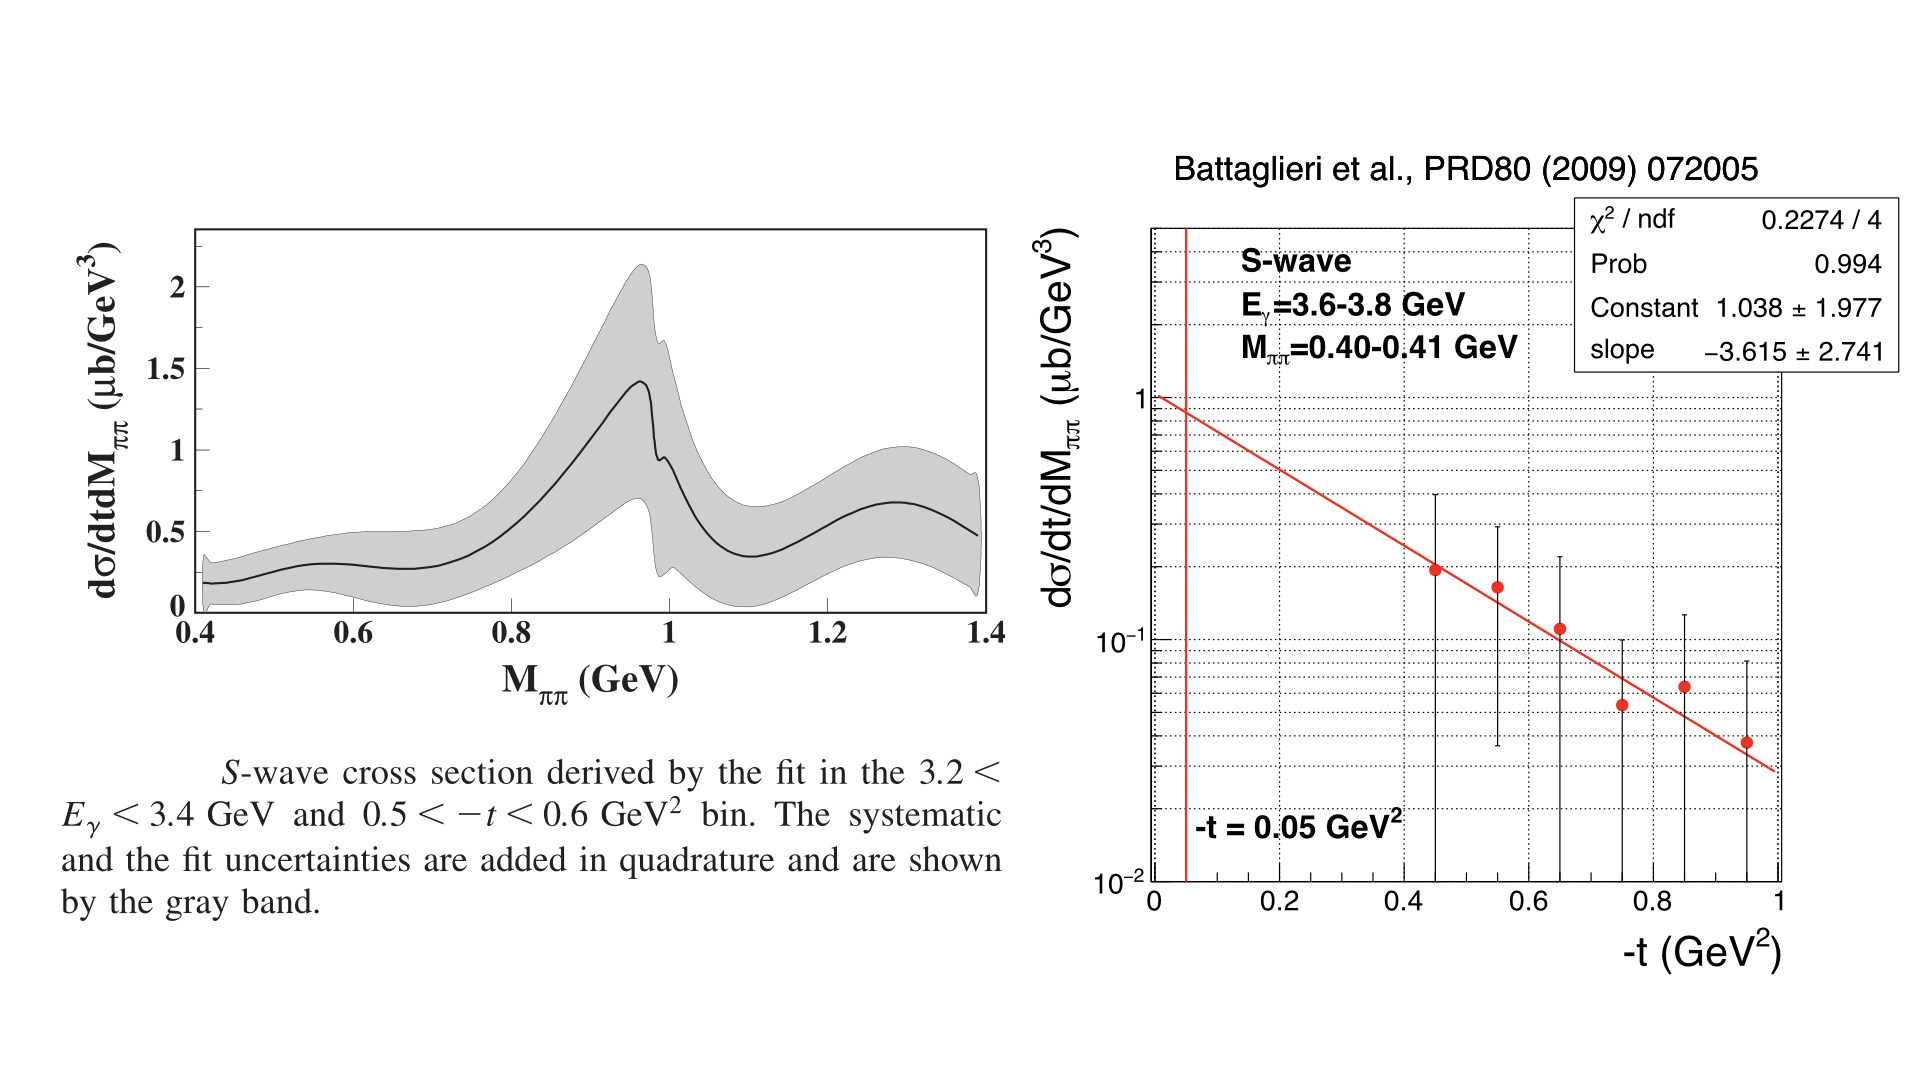
\includegraphics[width=6in]{figures/f0_500.png}
\caption{CLAS data for s-wave $\pi^+ \pi^-$ photoproduction on the proton at $3.2 < E_\gamma < 3.4$ GeV \cite{Battaglieri:2009aa}. }
\label{f0_500}
\end{figure}

\begin{figure}
\centering
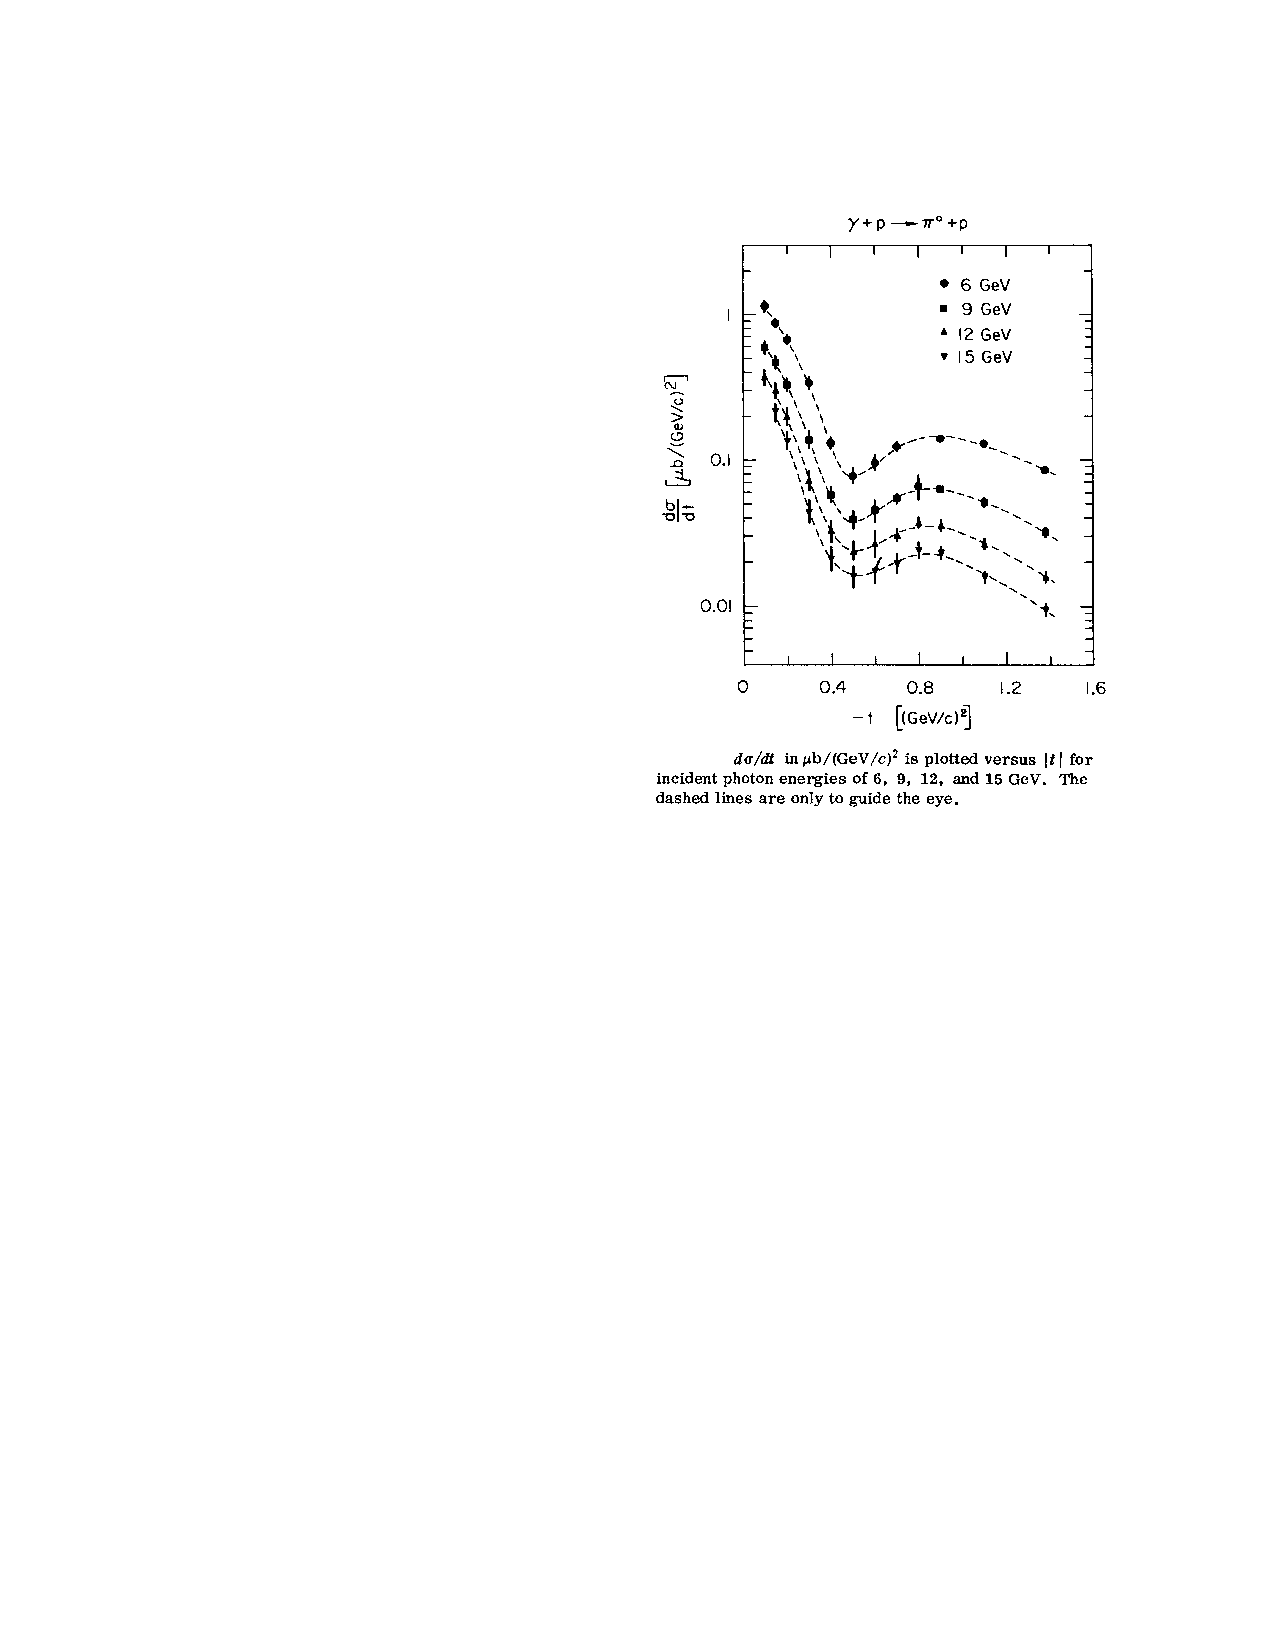
\includegraphics[width=4in]{figures/SLAC_data.pdf}
\caption{SLAC data for $\pi^0$ photo-production on the proton \cite{Anderson:1971}.}
\label{SLAC}
\end{figure}


\end{document}
